\documentclass[]{article}
\usepackage{lmodern}
\usepackage{amssymb,amsmath}
\usepackage{ifxetex,ifluatex}
\usepackage{fixltx2e} % provides \textsubscript
\ifnum 0\ifxetex 1\fi\ifluatex 1\fi=0 % if pdftex
  \usepackage[T1]{fontenc}
  \usepackage[utf8]{inputenc}
\else % if luatex or xelatex
  \ifxetex
    \usepackage{mathspec}
  \else
    \usepackage{fontspec}
  \fi
  \defaultfontfeatures{Ligatures=TeX,Scale=MatchLowercase}
\fi
% use upquote if available, for straight quotes in verbatim environments
\IfFileExists{upquote.sty}{\usepackage{upquote}}{}
% use microtype if available
\IfFileExists{microtype.sty}{%
\usepackage{microtype}
\UseMicrotypeSet[protrusion]{basicmath} % disable protrusion for tt fonts
}{}
\usepackage[margin=1in]{geometry}
\usepackage{hyperref}
\hypersetup{unicode=true,
            pdftitle={Modeling Dicamba Injury in non-Xtend Soybeans},
            pdfborder={0 0 0},
            breaklinks=true}
\urlstyle{same}  % don't use monospace font for urls
\usepackage{longtable,booktabs}
\usepackage{graphicx,grffile}
\makeatletter
\def\maxwidth{\ifdim\Gin@nat@width>\linewidth\linewidth\else\Gin@nat@width\fi}
\def\maxheight{\ifdim\Gin@nat@height>\textheight\textheight\else\Gin@nat@height\fi}
\makeatother
% Scale images if necessary, so that they will not overflow the page
% margins by default, and it is still possible to overwrite the defaults
% using explicit options in \includegraphics[width, height, ...]{}
\setkeys{Gin}{width=\maxwidth,height=\maxheight,keepaspectratio}
\IfFileExists{parskip.sty}{%
\usepackage{parskip}
}{% else
\setlength{\parindent}{0pt}
\setlength{\parskip}{6pt plus 2pt minus 1pt}
}
\setlength{\emergencystretch}{3em}  % prevent overfull lines
\providecommand{\tightlist}{%
  \setlength{\itemsep}{0pt}\setlength{\parskip}{0pt}}
\setcounter{secnumdepth}{5}
% Redefines (sub)paragraphs to behave more like sections
\ifx\paragraph\undefined\else
\let\oldparagraph\paragraph
\renewcommand{\paragraph}[1]{\oldparagraph{#1}\mbox{}}
\fi
\ifx\subparagraph\undefined\else
\let\oldsubparagraph\subparagraph
\renewcommand{\subparagraph}[1]{\oldsubparagraph{#1}\mbox{}}
\fi

%%% Use protect on footnotes to avoid problems with footnotes in titles
\let\rmarkdownfootnote\footnote%
\def\footnote{\protect\rmarkdownfootnote}

%%% Change title format to be more compact
\usepackage{titling}

% Create subtitle command for use in maketitle
\newcommand{\subtitle}[1]{
  \posttitle{
    \begin{center}\large#1\end{center}
    }
}

\setlength{\droptitle}{-2em}

  \title{Modeling Dicamba Injury in non-Xtend Soybeans}
    \pretitle{\vspace{\droptitle}\centering\huge}
  \posttitle{\par}
  \subtitle{Data analysis from Wisconsin, Michigan, Nebraska, Arkansas, Indiana, and
Ontario}
  \author{Max Oliveira\textsuperscript{1}, Guilherme Alves\textsuperscript{2}, and
Rodrigo Werle\textsuperscript{1}\\
\textsuperscript{1} University of Wisconsin-Madison\\
\textsuperscript{2} University of Nebraska-Lincoln}
    \preauthor{\centering\large\emph}
  \postauthor{\par}
    \date{}
    \predate{}\postdate{}
  
\usepackage{booktabs}
\usepackage{longtable}
\usepackage{array}
\usepackage{multirow}
\usepackage[table]{xcolor}
\usepackage{wrapfig}
\usepackage{float}
\usepackage{colortbl}
\usepackage{pdflscape}
\usepackage{tabu}
\usepackage{threeparttable}
\usepackage{threeparttablex}
\usepackage[normalem]{ulem}
\usepackage{makecell}

\begin{document}
\maketitle

\begin{center}\includegraphics[width=0.8\linewidth]{injury} \end{center}

\newpage 

\tableofcontents  \newpage  \listoffigures
\newpage  \listoftables
\newpage

\section{PROJECT LEADER}\label{project-leader}

\subsection{Bayer Crop Science}\label{bayer-crop-science}

\textbf{Bayer Crop Science}:
\href{https://www.cropscience.bayer.com/en}{Dr.~Ryan Rector}

\subsection{Arkansas}\label{arkansas}

\textbf{University of Arkansas}:
\href{https://crop-soil-environmental-sciences.uark.edu/directory/index/uid/jnorswor/name/Jason-Norsworthy/}{Dr.~Jason
Norsworthy}

\subsection{Indiana}\label{indiana}

\textbf{Purdue University}:
\href{https://ag.purdue.edu/btny/Pages/profile.aspx?strAlias=young285}{Dr.~Bryan
Young}

\subsection{Michigan}\label{michigan}

\textbf{Michigan State University}:
\href{https://www.canr.msu.edu/people/christy_sprague}{Dr.~Christy
Sprage}

\subsection{Nebraska}\label{nebraska}

\textbf{University of Nebraska-Lincoln}:
\href{https://agronomy.unl.edu/kruger}{Dr.~Greg Kruger}

\subsection{Ontario}\label{ontario}

\textbf{University of Guelph}:
\href{https://www.plant.uoguelph.ca/psikkema}{Dr.~Peter Sikkema}

\subsection{Wisconsin}\label{wisconsin}

\textbf{University of Wisconsin-Madison}:
\href{http://www.wiscweeds.info/}{Dr.~Rodrigo Werle}

\newpage

\section{ARKANSAS}\label{arkansas-1}

\subsection{Location}\label{location}

The study was conducted in a soybean field at Proctor, Arkansas (Figure
1)

\begin{figure}[h]

{\centering 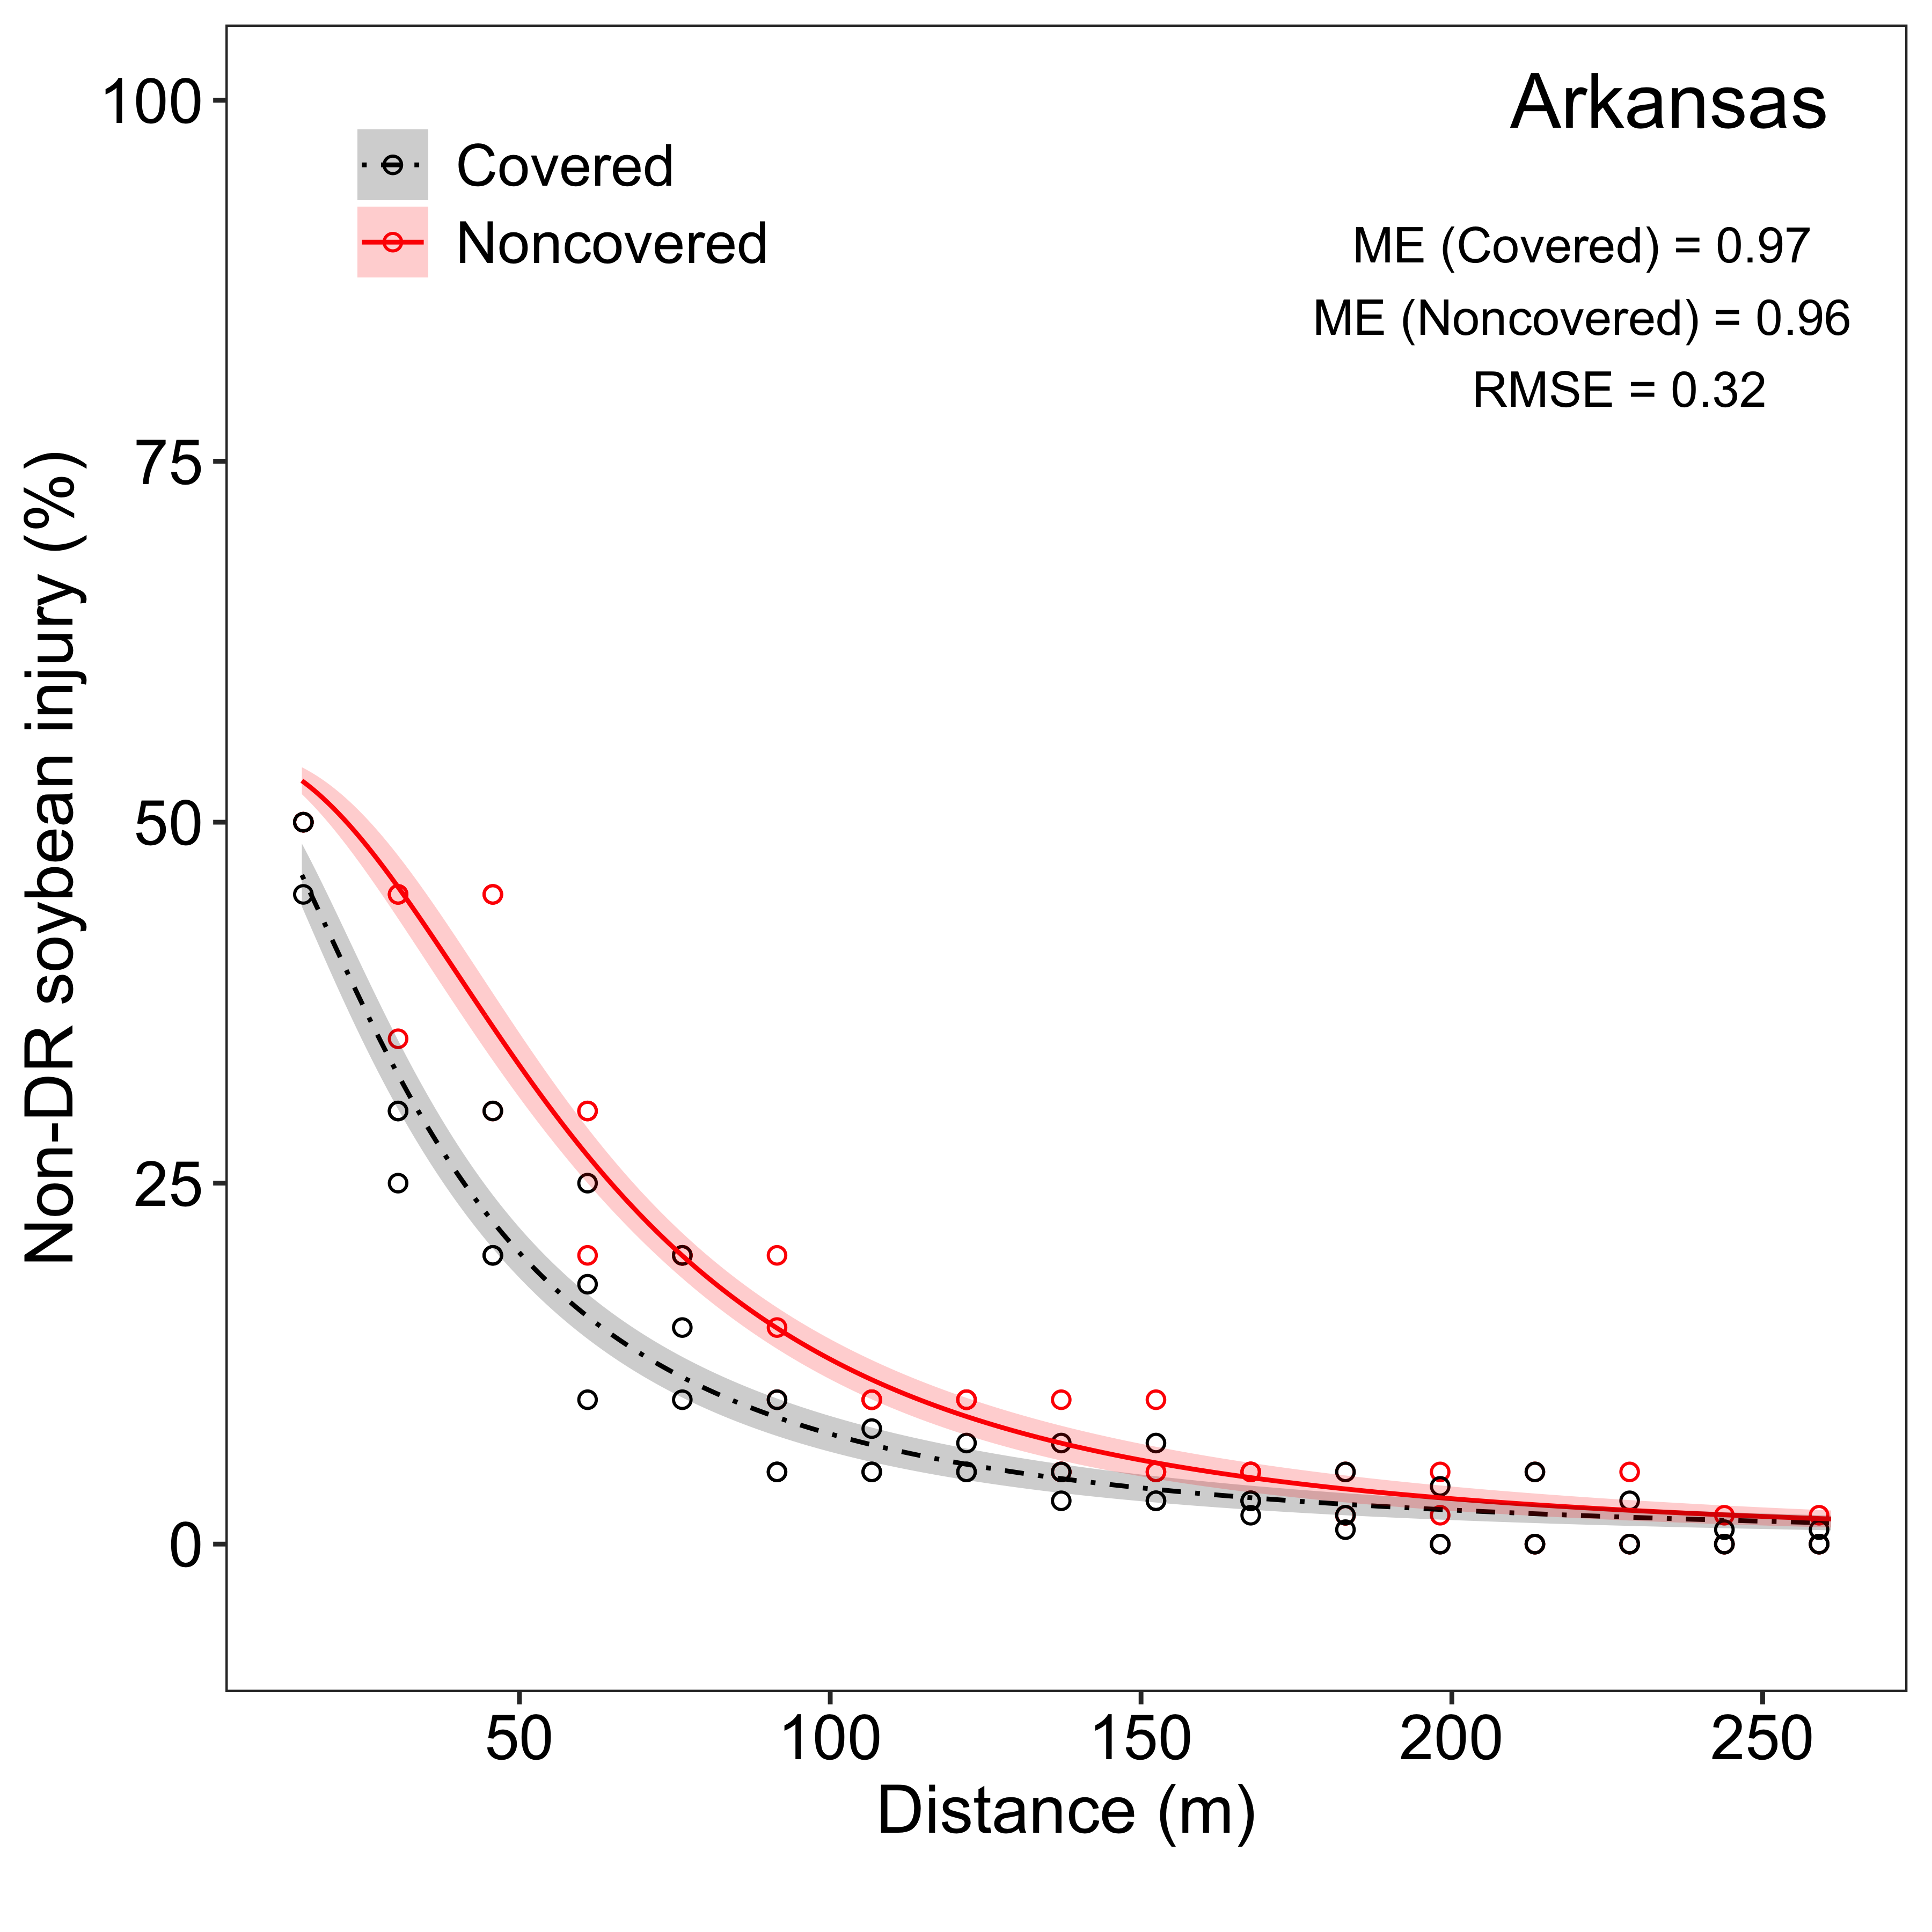
\includegraphics[width=1\linewidth]{Arkansas} 

}

\caption{Aerial view of the large scale volatility trial in Arkansas.}\label{fig:unnamed-chunk-4}
\end{figure}

\newpage

\subsection{Modeling}\label{modeling}

Non-Xtend \textbf{soybean injury (\%)} (visual data) from Arkansas
presented here was collected in from one soybean plant
distance\textsuperscript{-1} at 22 and 29 days after treatment (DAT) but
without replication. Nonetheless, we use the three-parameter logistic
model (Equation 1) for fitting soybean injury (\%) with distance from
the area treated with dicamba.

Equation 1: \[Y= \frac{d}{(1 + exp[b(logx - loge)]} \]

where \emph{Y} is the soybean injury (\%), \emph{x} is the distance (m)
from the dicamba treated area. in The parameter \emph{d} is the upper
limit (asymptote), \emph{b} is the slope and the parameter \emph{e} is
the ED50 (effective \emph{x} that causes 50\% reduction in \emph{Y}).
Data from 22 and 29 DAT are presented.

Non-Xtend \textbf{soybean height} (cm) from Arkansas presented here was
collected from 10 soybean plant distance\textsuperscript{-1} at 22 DAT.
\emph{Loess} local regression was fitted to the data.

\pagebreak
\newpage

\subsection{Wind}\label{wind}

Frequency of wind direction and speed (m/s) three days after dicamaba
application (Figure X).

\begin{figure}
\centering
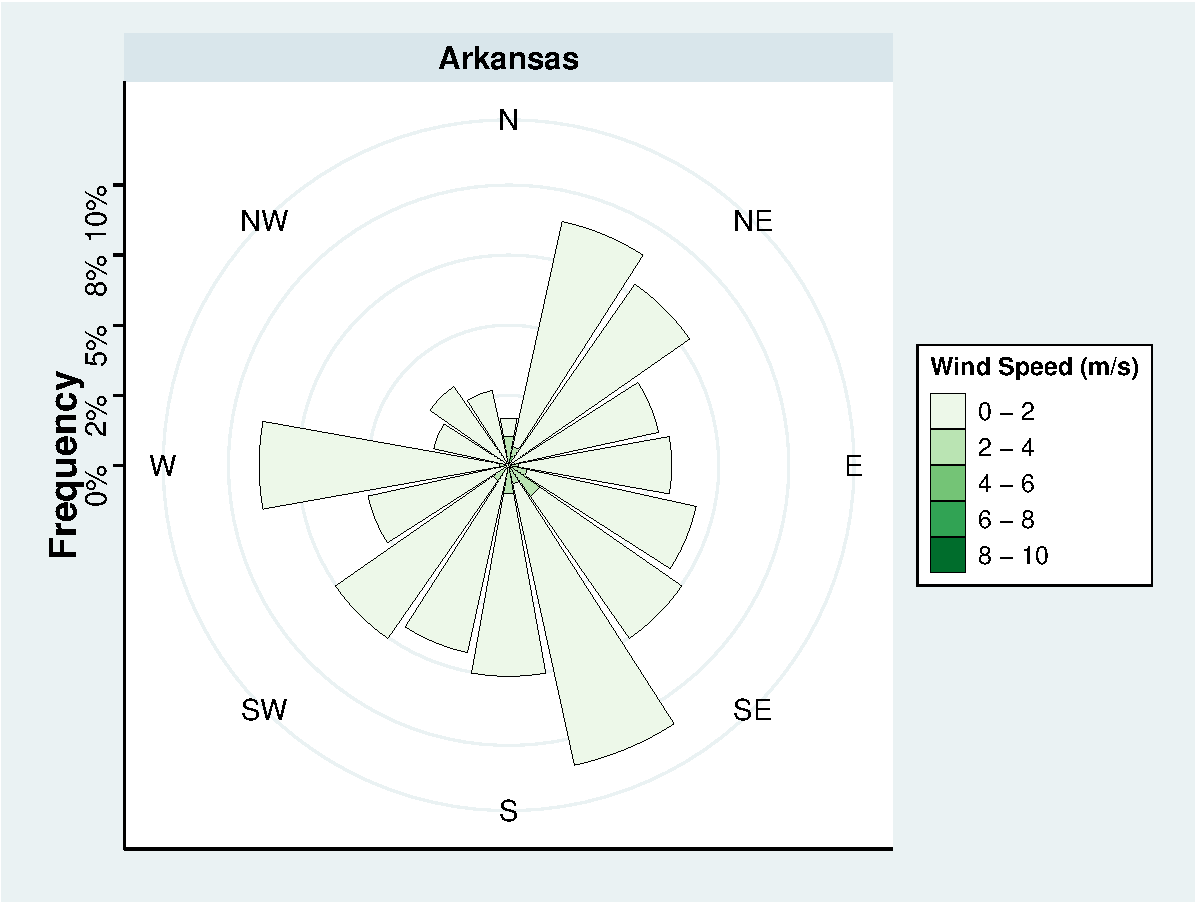
\includegraphics{Report_Dicamba_study_files/figure-latex/unnamed-chunk-6-1.pdf}
\caption{Wind rose plots demonstrating the average wind frequency (\%)
and wind speed (m s\textsuperscript{1}) grouped in 22.5° of direction
(from which the wind is blowing) in Arkansas.}
\end{figure}

\pagebreak
\newpage

\subsection{Transects}\label{transects}

\pagebreak
\newpage

\subsection{Results at 22 DAT}\label{results-at-22-dat}

\subsubsection{Dicamba injury (\%) in non-Xtend
soybeans}\label{dicamba-injury-in-non-xtend-soybeans}

\paragraph{\texorpdfstring{Area located in the \textbf{upwind} direction
1, 2, and
3}{Area located in the upwind direction 1, 2, and 3}}\label{area-located-in-the-upwind-direction-1-2-and-3}

\begin{longtable}[]{@{}lllll@{}}
\caption{Parameters of the log-logistic model at west upwind transects
(1, 2, and 3) at 22 DAT in Arkansas.}\tabularnewline
\toprule
Parameter & Transect & Estimate (± SE) & t-value &
p-value\tabularnewline
\midrule
\endfirsthead
\toprule
Parameter & Transect & Estimate (± SE) & t-value &
p-value\tabularnewline
\midrule
\endhead
Slope & West Transect 1 & 3.99 ± 1.13 & 3.51 & 0.02 *\tabularnewline
Slope & West Transect 2 & 3.87 ± 1.12 & 3.45 & 0.02 *\tabularnewline
Slope & West Transect 3 & 1.84 ± 0.88 & 2.08 & 0.10\tabularnewline
Asymptote & West Transect 1 & 44.92 ± 5.81 & 7.73 & 0.00
**\tabularnewline
Asymptote & West Transect 2 & 52.59 ± 8.63 & 6.09 & 0.00
**\tabularnewline
Asymptote & West Transect 3 & 117.40 ± 353.09 & 0.33 & 0.75
***\tabularnewline
ED50 & West Transect 1 & 25.73 ± 3.11 & 8.25 & 0.00 **\tabularnewline
ED50 & West Transect 2 & 24.12 ± 3.59 & 6.71 & 0.00 **\tabularnewline
ED50 & West Transect 3 & 8.54 ± 20.73 & 0.41 & 0.70\tabularnewline
\bottomrule
\end{longtable}

\begin{longtable}[]{@{}llll@{}}
\caption{Estimation of the distance (m) that resulted in 1 (ED1), 10
(ED10), and 20\% (ED20) injury on non-Xtend soybeans at westupwind
transects (1, 2, and 3) at 22 DAT in Arkansas.}\tabularnewline
\toprule
Transect & ED1 (m) (± SE) & ED10 (m) (± SE) & ED20 (m) (±
SE)\tabularnewline
\midrule
\endfirsthead
\toprule
Transect & ED1 (m) (± SE) & ED10 (m) (± SE) & ED20 (m) (±
SE)\tabularnewline
\midrule
\endhead
West Transect 1 & 66.36 ± 11.30 & 35.20 ± 2.04 & 27.19 ±
2.92\tabularnewline
West Transect 2 & 66.82 ± 11.08 & 35.07 ± 2.19 & 27.36 ±
3.16\tabularnewline
West Transect 3 & 111.95 ± 140.36 & 30.85 ± 56.57 & 20.11 ±
40.84\tabularnewline
\bottomrule
\end{longtable}

\begin{longtable}[]{@{}llll@{}}
\caption{Comparison of EDs among west upwind transects (1, 2, and 3) at
22 DAT in Arkansas.}\tabularnewline
\toprule
Comparison & Estimate (± SE) & t-value & p-value\tabularnewline
\midrule
\endfirsthead
\toprule
Comparison & Estimate (± SE) & t-value & p-value\tabularnewline
\midrule
\endhead
West Transect 1/West Transect 2:E1/E1 & 0.99 ± 0.23 & -0.02 &
0.97\tabularnewline
West Transect 1/West Transect 3:E1/E1 & 0.59 ± 0.75 & -0.53 &
0.61\tabularnewline
West Transect 2/West Transect 3:E1/E1 & 0.59 ± 0.76 & -0.53 &
0.62\tabularnewline
West Transect 1/West Transect 2:E10/E10 & 1.00 ± 0.08 & 0.04 &
0.96\tabularnewline
West Transect 1/West Transect 3:E10/E10 & 1.14 ± 2.11 & 0.06 &
0.94\tabularnewline
West Transect 2/West Transect 3:E10/E10 & 1.13 ± 2.10 & 0.06 &
0.95\tabularnewline
West Transect 1/West Transect 2:E20/E20 & 0.99 ± 0.15 & -0.04 &
0.96\tabularnewline
West Transect 1/West Transect 3:E20/E20 & 1.35 ± 2.77 & 0.12 &
0.90\tabularnewline
West Transect 2/West Transect 3:E20/E20 & 1.36 ± 2.79 & 0.13 &
0.90\tabularnewline
\bottomrule
\end{longtable}

\begin{figure}
\centering
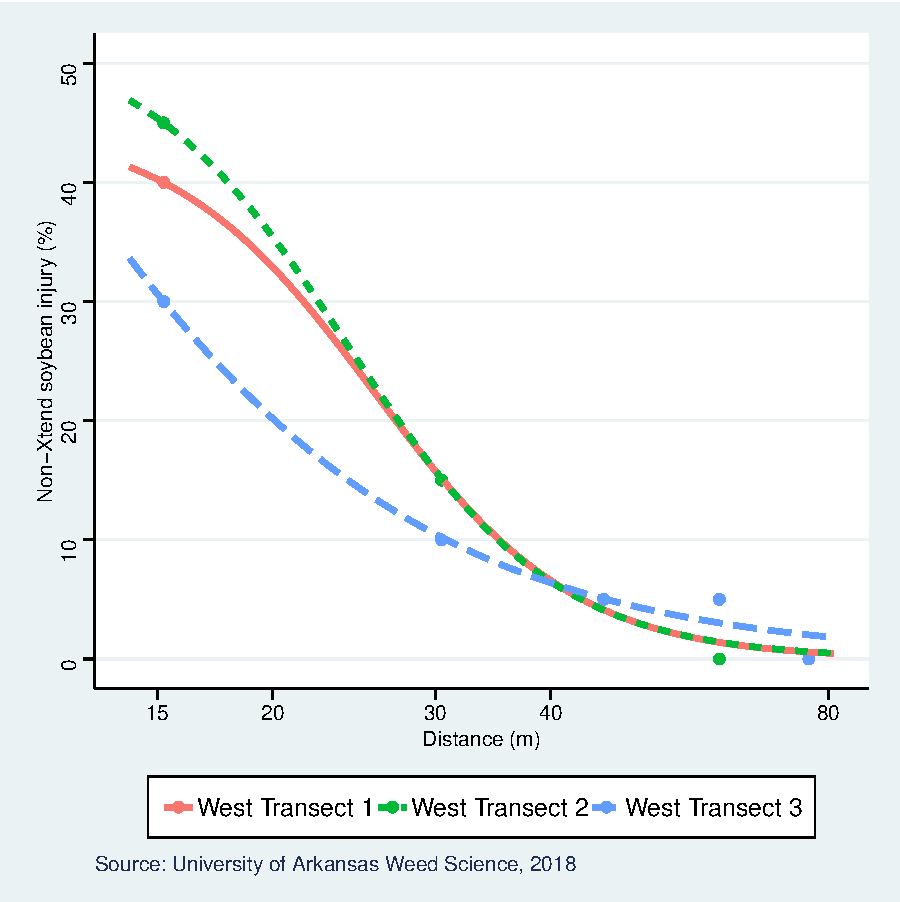
\includegraphics{Report_Dicamba_study_files/figure-latex/unnamed-chunk-9-1.pdf}
\caption{Non-Xtend soybean injury (\%) with distance (\%) from the
dicamba treated area in the upwind west transect 1, 2, and 3 in Arkansas
at 22 DAT.}
\end{figure}

\pagebreak
\newpage

\paragraph{\texorpdfstring{Area located in the \textbf{downwind}
direction 1, 2, and
3.}{Area located in the downwind direction 1, 2, and 3.}}\label{area-located-in-the-downwind-direction-1-2-and-3.}

\begin{longtable}[]{@{}lllll@{}}
\caption{Parameters of the log-logistic model at east downwind transects
(1, 2, and 3) at 22 DAT in Arkansas.}\tabularnewline
\toprule
Parameter & Transect & Estimate (± SE) & t-value &
p-value\tabularnewline
\midrule
\endfirsthead
\toprule
Parameter & Transect & Estimate (± SE) & t-value &
p-value\tabularnewline
\midrule
\endhead
Slope & East Transect 1 & 3.44 ± 0.35 & 9.60 & 0.00 ***\tabularnewline
Slope & East Transect 2 & 2.46 ± 0.22 & 10.82 & 0.00 ***\tabularnewline
Slope & East Transect 3 & 2.03 ± 0.22 & 9.26 & 0.00 ***\tabularnewline
Asymptote & East Transect 1 & 50.26 ± 1.97 & 25.47 & 0.00
***\tabularnewline
Asymptote & East Transect 2 & 52.20 ± 2.35 & 22.18 & 0.00
***\tabularnewline
Asymptote & East Transect 3 & 51.90 ± 4.07 & 12.72 & 0.00
***\tabularnewline
ED50 & East Transect 1 & 69.44 ± 2.95 & 23.47 & 0.00 ***\tabularnewline
ED50 & East Transect 2 & 71.08 ± 4.18 & 17.00 & 0.00 ***\tabularnewline
ED50 & East Transect 3 & 52.02 ± 6.01 & 8.64 & 0.00 ***\tabularnewline
\bottomrule
\end{longtable}

\begin{longtable}[]{@{}llll@{}}
\caption{Estimation of the distance (m) that resulted in 1 (ED1), 10
(ED10), and 20\% (ED20) injury on non-Xtend soybeans at east downwind
transects (1, 2, and 3) at 22 DAT in Arkansas.}\tabularnewline
\toprule
Transect & ED1 (m) (± SE) & ED10 (m) (± SE) & ED20 (m) (±
SE)\tabularnewline
\midrule
\endfirsthead
\toprule
Transect & ED1 (m) (± SE) & ED10 (m) (± SE) & ED20 (m) (±
SE)\tabularnewline
\midrule
\endhead
West Transect 1 & 215.55 ± 22.21 & 104.09 ± 4.36 & 78.32 ±
2.95\tabularnewline
West Transect 2 & 350.70 ± 41.41 & 127.46 ± 6.04 & 86.23 ±
4.23\tabularnewline
West Transect 3 & 358.72 ± 47.04 & 105.18 ± 7.22 & 65.44 ±
6.30\tabularnewline
\bottomrule
\end{longtable}

\begin{longtable}[]{@{}llll@{}}
\caption{Comparison of EDs among east downwind transects (1, 2, and 3)
at 22 DAT in Arkansas.}\tabularnewline
\toprule
Comparison & Estimate (± SE) & t-value & p-value\tabularnewline
\midrule
\endfirsthead
\toprule
Comparison & Estimate (± SE) & t-value & p-value\tabularnewline
\midrule
\endhead
EastTransect 1/East Transect 2:E1/E1 & 0.61 ± 0.09 & -4.00 &
0.00\tabularnewline
East Transect 1/East Transect 3:E1/E1 & 0.60 ± 0.10 & -3.98 &
0.00\tabularnewline
East Transect 2/East Transect 3:E1/E1 & 0.97 ± 0.17 & -0.12 &
0.89\tabularnewline
East Transect 1/East Transect 2:E10/E10 & 0.81 ± 0.05 & -3.54 &
0.00\tabularnewline
East Transect 1/East Transect 3:E10/E10 & 0.98 ± 0.07 & -0.12 &
0.89\tabularnewline
East Transect 2/East Transect 3:E10/E10 & 1.21 ± -0.10 & 2.09 &
0.04\tabularnewline
East Transect 1/East Transect 2:E20/E20 & 0.90 ± 0.05 & -1.63 &
0.11\tabularnewline
East Transect 1/East Transect 3:E20/E20 & 1.19 ± 0.12 & 1.58 &
-0.11\tabularnewline
East Transect 2/East Transect 3:E20/E20 & 1.32 ± 0.14 & 2.22 &
-0.03\tabularnewline
\bottomrule
\end{longtable}

\begin{figure}
\centering
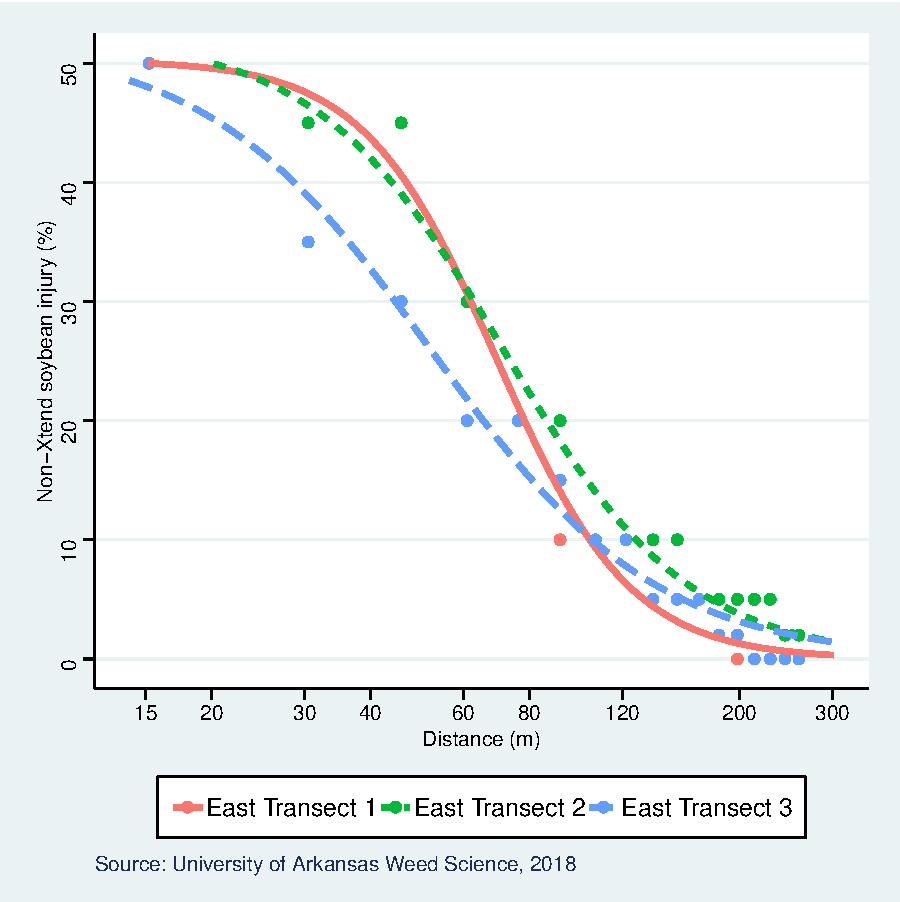
\includegraphics{Report_Dicamba_study_files/figure-latex/unnamed-chunk-12-1.pdf}
\caption{Non-Xtend soybean injury (\%) with distance (m) from the
dicamba treated area in the downwind east transect 1, 2, and 3 in
Arkansas at 22 DAT.}
\end{figure}

\newpage

\subsubsection{Non-Xtend soybeans
height}\label{non-xtend-soybeans-height}

\paragraph{\texorpdfstring{Area located in the \textbf{upwind} direction
1, 2, and
3}{Area located in the upwind direction 1, 2, and 3}}\label{area-located-in-the-upwind-direction-1-2-and-3-1}

\begin{figure}
\centering
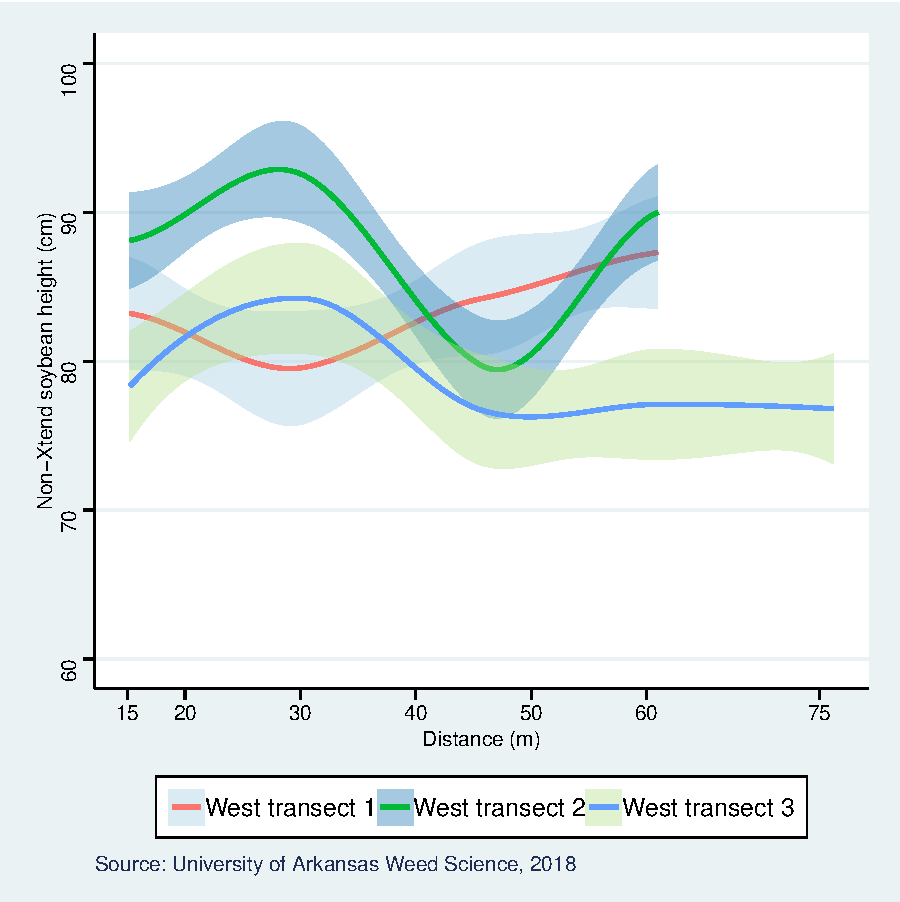
\includegraphics{Report_Dicamba_study_files/figure-latex/unnamed-chunk-14-1.pdf}
\caption{Non-Xtend soybean height (cm) with distance (m) from the
dicamba treated area in the upwind west transect 1, 2, and 3 in Arkansas
at 22 DAT.}
\end{figure}

\pagebreak
\newpage

\paragraph{Non-Xtend soybeans height}\label{non-xtend-soybeans-height-1}

\paragraph{\texorpdfstring{Area located in the \textbf{downwind}
direction 1, 2, and
3}{Area located in the downwind direction 1, 2, and 3}}\label{area-located-in-the-downwind-direction-1-2-and-3}

\begin{figure}
\centering
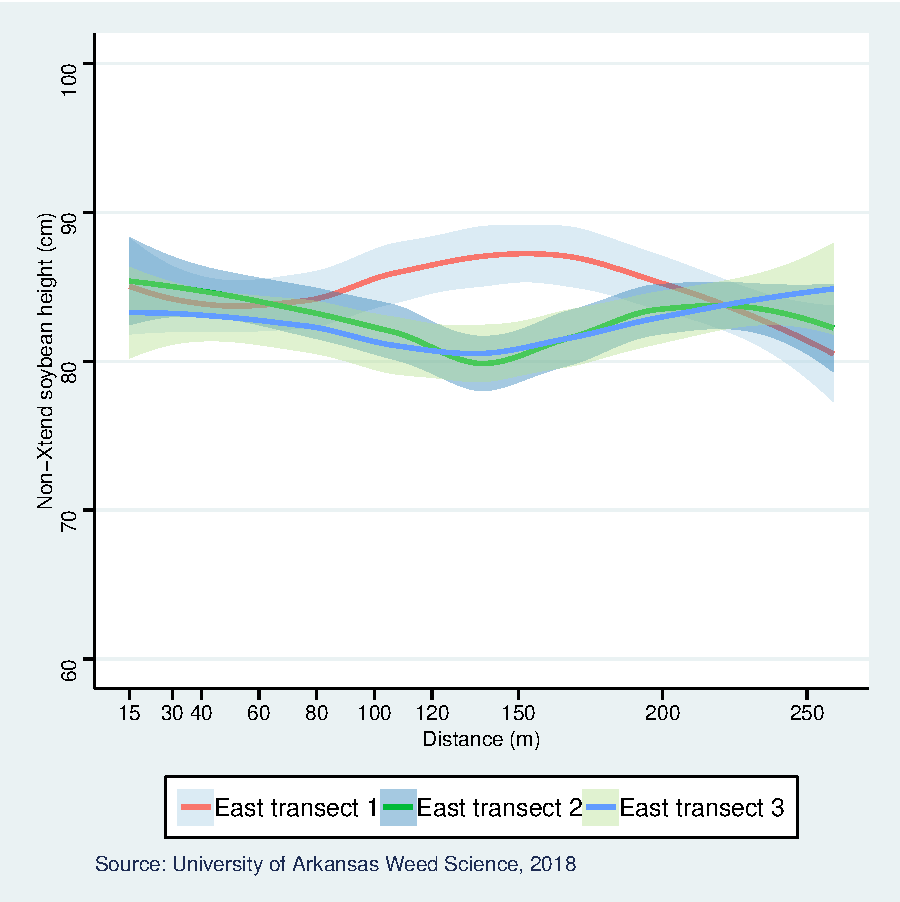
\includegraphics{Report_Dicamba_study_files/figure-latex/unnamed-chunk-16-1.pdf}
\caption{Non-Xtend soybean injury (\%) with distance (m) from the
dicamba treated area in the downwind east transect 1, 2, and 3 in
Arkansas at 22 DAT.}
\end{figure}

\pagebreak
\newpage

\subsection{Results at 29 DAT}\label{results-at-29-dat}

\subsubsection{Dicamba injury (\%) in non-Xtend
soybeans}\label{dicamba-injury-in-non-xtend-soybeans-1}

\begin{longtable}[]{@{}lllll@{}}
\caption{Parameters of the log-logistic model of four sides of the
treated area (N, E, S, W) at 29 DAT in Arkansas.}\tabularnewline
\toprule
Parameter & Transect & Estimate (± SE) & t-value &
p-value\tabularnewline
\midrule
\endfirsthead
\toprule
Parameter & Transect & Estimate (± SE) & t-value &
p-value\tabularnewline
\midrule
\endhead
Slope & N & 7.25 ± 1.75 & 4.13 & 0.00 ***\tabularnewline
Slope & E & 1.82 ± 0.26 & 6.81 & 0.00 ***\tabularnewline
Slope & S & 2.62 ± 0.28 & 9.10 & 0.00 ***\tabularnewline
Slope & W & 2.22 ± 0.32 & 6.95 & 0.00 ***\tabularnewline
Asymptote & N & 45.54 ± 0.92 & 48.99 & 0.00 ***\tabularnewline
Asymptote & E & 73.78 ± 12.36 & 5.96 & 0.00 ***\tabularnewline
Asymptote & S & 57.18 ± 2.96 & 19.28 & 0.00 ***\tabularnewline
Asymptote & W & 51.45 ± 4.65 & 11.05 & 0.00 ***\tabularnewline
ED50 & N & 273.69 ± 7.41 & 36.91 & 0.00 ***\tabularnewline
ED50 & E & 27.77 ± 6.36 & 4.36 & 0.00 ***\tabularnewline
ED50 & S & 62.73 ± 4.09 & 15.30 & 0.00 ***\tabularnewline
ED50 & W & 42.61 ± 5.06 & 8.42 & 0.00 ***\tabularnewline
\bottomrule
\end{longtable}

\begin{longtable}[]{@{}llll@{}}
\caption{Estimation of the distance (m) that resulted in 1 (ED1), 10
(ED10), and 20\% (ED20) injury on non-Xtend soybeans of four sides of
the treated area (N, E, S, W) at 29 DAT in Arkansas.}\tabularnewline
\toprule
Transect & ED1 (m) (± SE) & ED10 (m) (± SE) & ED20 (m) (±
SE)\tabularnewline
\midrule
\endfirsthead
\toprule
Transect & ED1 (m) (± SE) & ED10 (m) (± SE) & ED20 (m) (±
SE)\tabularnewline
\midrule
\endhead
N & 461.94 ± 67.33 & 325.98 ± 20.67 & 283.10 ± 9.34\tabularnewline
E & 292.17 ± 50.04 & 76.79 ± 8.82 & 47.80 ± 7.70\tabularnewline
S & 291.65 ± 39.08 & 113.37 ± 5.99 & 79.47 ± 4.10\tabularnewline
W & 247.68 ± 44.95 & 80.67 ± 6.31 & 52.21 ± 5.15\tabularnewline
\bottomrule
\end{longtable}

\newpage

\begin{longtable}[]{@{}llll@{}}
\caption{Comparison of EDs among four sides of the treated area (N, E,
S, W) at 29 DAT in Arkansas.}\tabularnewline
\toprule
Comparison & Estimate (± SE) & t-value & p-value\tabularnewline
\midrule
\endfirsthead
\toprule
Comparison & Estimate (± SE) & t-value & p-value\tabularnewline
\midrule
\endhead
E/N:ED1/ED1 & 0.63 ± 0.14 & -2.58 & 0.01\tabularnewline
E/S:ED1/ED1 & 1.00 ± 0.21 & 0.00 & 0.99\tabularnewline
E/W:ED1/ED1 & 1.17 ± 0.29 & 0.61 & 0.54\tabularnewline
N/S:ED1/ED1 & 1.58 ± 0.31 & 1.86 & 0.06\tabularnewline
N/W:ED1/ED1 & 1.86 ± 0.43 & 1.99 & 0.05\tabularnewline
S/W:ED1/ED1 & 1.17 ± 0.26 & 0.66 & 0.50\tabularnewline
E/N:ED10/ED10 & 0.23 ± 0.03 & -24.7 & 0.00\tabularnewline
E/S:ED10/ED10 & 0.67 ± 0.08 & -3.76 & 0.00\tabularnewline
E/W:ED10/ED10 & 0.95 ± 0.13 & -0.36 & 0.71\tabularnewline
N/S:ED10/ED10 & 2.87 ± 0.23 & 7.90 & 0.00\tabularnewline
N/W:ED10/ED10 & 4.04 ± 0.40 & 7.46 & 0.00\tabularnewline
S/W:ED10/ED10 & 1.40 ± 0.13 & 3.05 & 0.00\tabularnewline
E/N:ED20/ED20 & 0.16 ± 0.02 & -2.99 & 0.00\tabularnewline
E/S:ED20/ED20 & 0.60 ± 0.10 & -3.91 & 0.00\tabularnewline
E/W:ED20/ED20 & 0.91 ± 0.17 & -0.48 & 0.06\tabularnewline
N/S:ED20/ED20 & 3.56 ± 0.21 & 1.17 & 0.00\tabularnewline
N/W:ED20/ED20 & 5.42 ± 0.56 & 7.83 & 0.00\tabularnewline
S/W:ED20/ED20 & 1.52 ± 0.16 & 3.08 & 0.00\tabularnewline
\bottomrule
\end{longtable}

\begin{figure}
\centering
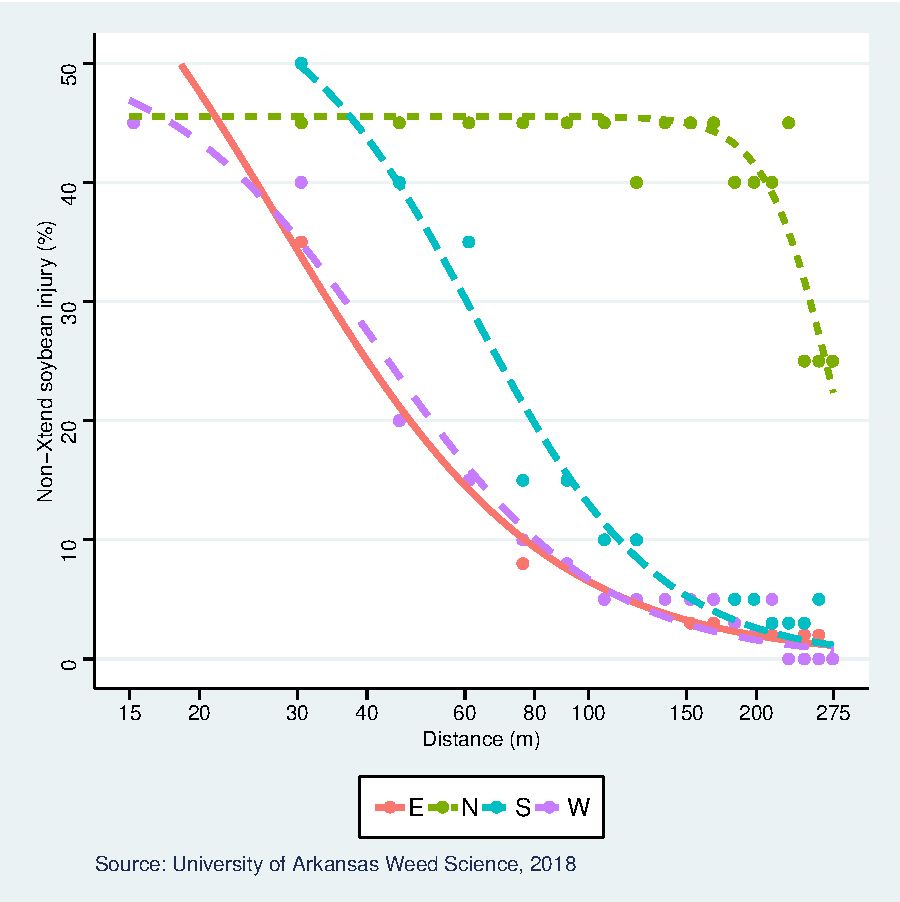
\includegraphics{Report_Dicamba_study_files/figure-latex/unnamed-chunk-19-1.pdf}
\caption{Non-Xtend soybean injury (\%) with distance (\%) from the
dicamba treated area of four sides of the treated area (N, E, S, W) at
29 DAT in Arkansas.}
\end{figure}

\newpage

\pagebreak

\section{INDIANA}\label{indiana-1}

\subsection{Location}\label{location-1}

The study was conducted in a soybean field at XXXXX of the Purdue
University (Figure X).

\begin{figure}[h]

{\centering 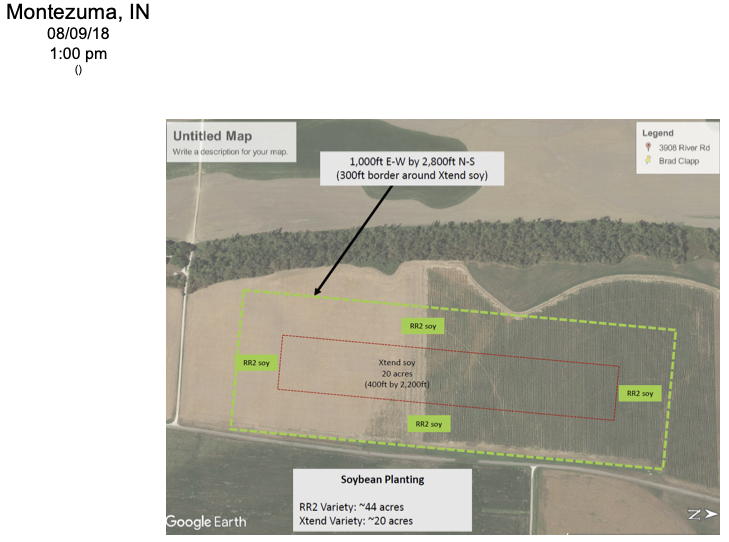
\includegraphics[width=1\linewidth]{Indiana} 

}

\caption{Aerial view of the large scale volatility trial in Indiana.}\label{fig:unnamed-chunk-21}
\end{figure}

\pagebreak
\newpage

\subsection{Modeling}\label{modeling-1}

Non-Xtend \textbf{soybean injury (\%)} (visual data) from Indiana
presented here was collected in from one soybean plant
distance\textsuperscript{-1} at 21 DAT but without replication.
Nonetheless, we use the three-parameter logistic model (Equation 1) for
fitting soybean injury (\%) with distance from the area treated with
dicamba.

Equation 1: \[Y= \frac{d}{(1 + exp[b(logx - loge)]} \]

where \emph{Y} is the soybean injury (\%), \emph{x} is the distance (m)
from the dicamba treated area. in The parameter \emph{d} is the upper
limit (asymptote), \emph{b} is the slope and the parameter \emph{e} is
the ED50 (effective \emph{x} that causes 50\% reduction in \emph{Y}).
The upper limit of the model is locked at 100. Only data recorded 21 DAT
is presented.

Non-Xtend \textbf{soybean height} (cm) from Arkansas presented here was
collected from 10 soybean plant distance\textsuperscript{-1} at 21 DAT.
\emph{Loess} local regression was fitted to the data.

\pagebreak
\newpage

\subsection{Wind}\label{wind-1}

Frequency of wind direction and speed (m/s) three days after dicamaba
application (Figure X).

\begin{figure}
\centering
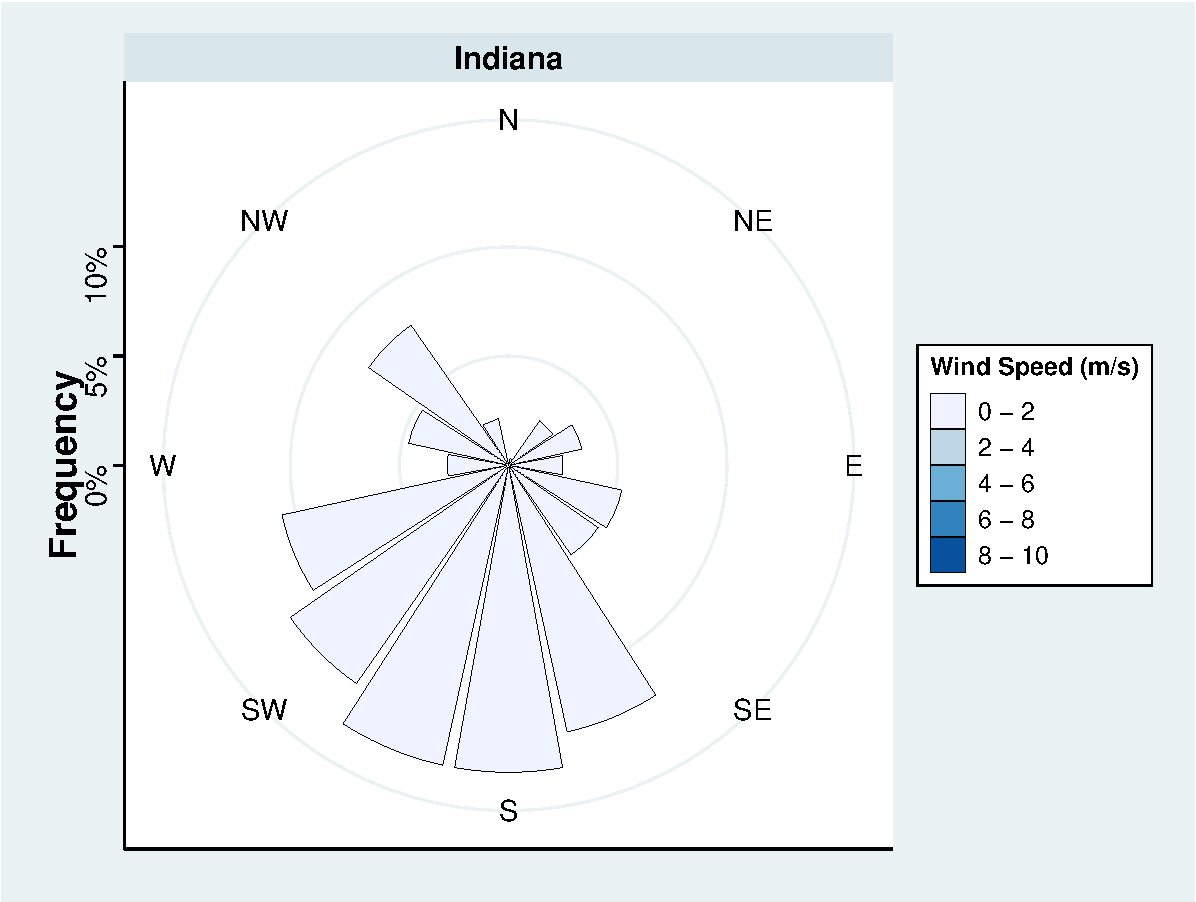
\includegraphics{Report_Dicamba_study_files/figure-latex/unnamed-chunk-23-1.pdf}
\caption{Wind rose plots demonstrating the average wind frequency (\%)
and wind speed (m s\textsuperscript{1}) grouped in 22.5° of direction
(from which the wind is blowing) in Indiana.}
\end{figure}

\pagebreak
\newpage

\subsection{Transects}\label{transects-1}

\begin{figure}[h]

{\centering 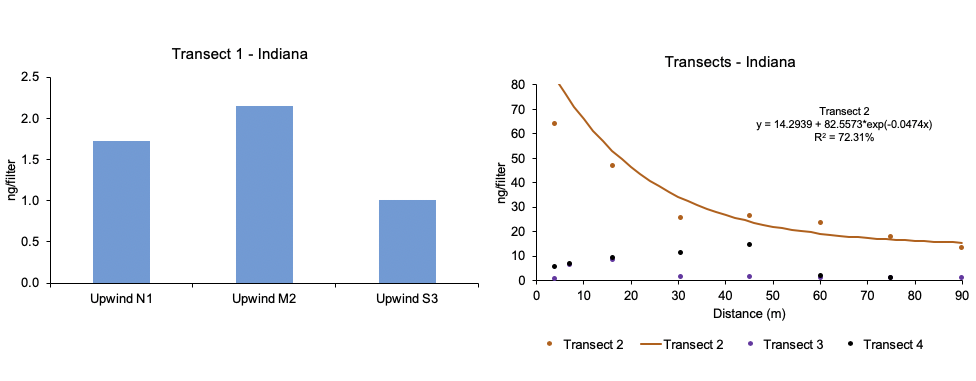
\includegraphics[width=1\linewidth]{INtransect} 

}

\caption{Deposition of dicamba particles at the transects in Indiana}\label{fig:unnamed-chunk-24}
\end{figure}

\pagebreak
\newpage

\subsection{Results at 21 DAT}\label{results-at-21-dat}

\subsubsection{Dicamba injury (\%) in non-Xtend
soybeans}\label{dicamba-injury-in-non-xtend-soybeans-2}

\paragraph{\texorpdfstring{Area located in the \textbf{North} direction
(cover and
uncover)}{Area located in the North direction (cover and uncover)}}\label{area-located-in-the-north-direction-cover-and-uncover}

\begin{longtable}[]{@{}lllll@{}}
\caption{Parameters of the log-logistic model of north direction (cover
and uncover) at 21 DAT in Indiana.}\tabularnewline
\toprule
Parameter & Area & Estimate (± SE) & t-value & p-value\tabularnewline
\midrule
\endfirsthead
\toprule
Parameter & Area & Estimate (± SE) & t-value & p-value\tabularnewline
\midrule
\endhead
Slope & Cover & 1.01 ± 0.68 & 1.47 & 0.16\tabularnewline
Slope & Uncover & 2.24 ± 0.29 & 7.72 & 0.00 ***\tabularnewline
Asymptote & Cover & 100 & &\tabularnewline
Asymptote & Uncover & 100 & &\tabularnewline
ED50 & Cover & 0.17 ± 0.32 & 0.54 & 0.59\tabularnewline
ED50 & Uncover & 2.71 ± 0.17 & 15.71 & 0.00 ***\tabularnewline
\bottomrule
\end{longtable}

\begin{longtable}[]{@{}llll@{}}
\caption{Estimation of the distance (m) that resulted in 1 (ED1), 10
(ED10), and 20\% (ED20) injury on non-Xtend soybeans of north direction
(cover and uncover) at 21 DAT in Indiana.}\tabularnewline
\toprule
Area & ED1 (m) (± SE) & ED10 (m) (± SE) & ED20 (m) (± SE)\tabularnewline
\midrule
\endfirsthead
\toprule
Area & ED1 (m) (± SE) & ED10 (m) (± SE) & ED20 (m) (± SE)\tabularnewline
\midrule
\endhead
Cover & 16.7 ± 23.13 & 1.55 ± 0.8 & 0.69 ± 0.66\tabularnewline
Uncover & 21.05 ± 5.43 & 7.23 ± 0.92 & 5.03 ± 0.45\tabularnewline
\bottomrule
\end{longtable}

\begin{longtable}[]{@{}llll@{}}
\caption{Comparison of EDs among four sides of north direction (cover
and uncover) at 21 DAT in Indiana.}\tabularnewline
\toprule
Comparison & Estimate (± SE) & t-value & p-value\tabularnewline
\midrule
\endfirsthead
\toprule
Comparison & Estimate (± SE) & t-value & p-value\tabularnewline
\midrule
\endhead
Cover/Uncover:ED1/ED1 & 0.21 ± 0.12 & -2.58 & 0.01\tabularnewline
Cover/Uncover:ED10/ED10 & 1.00 ± 0.21 & 6.55 & 0.00\tabularnewline
Cover/Uncover:ED20/ED20 & 0.14 ± 0.13 & -6.47 & 0.00\tabularnewline
\bottomrule
\end{longtable}

\begin{figure}
\centering
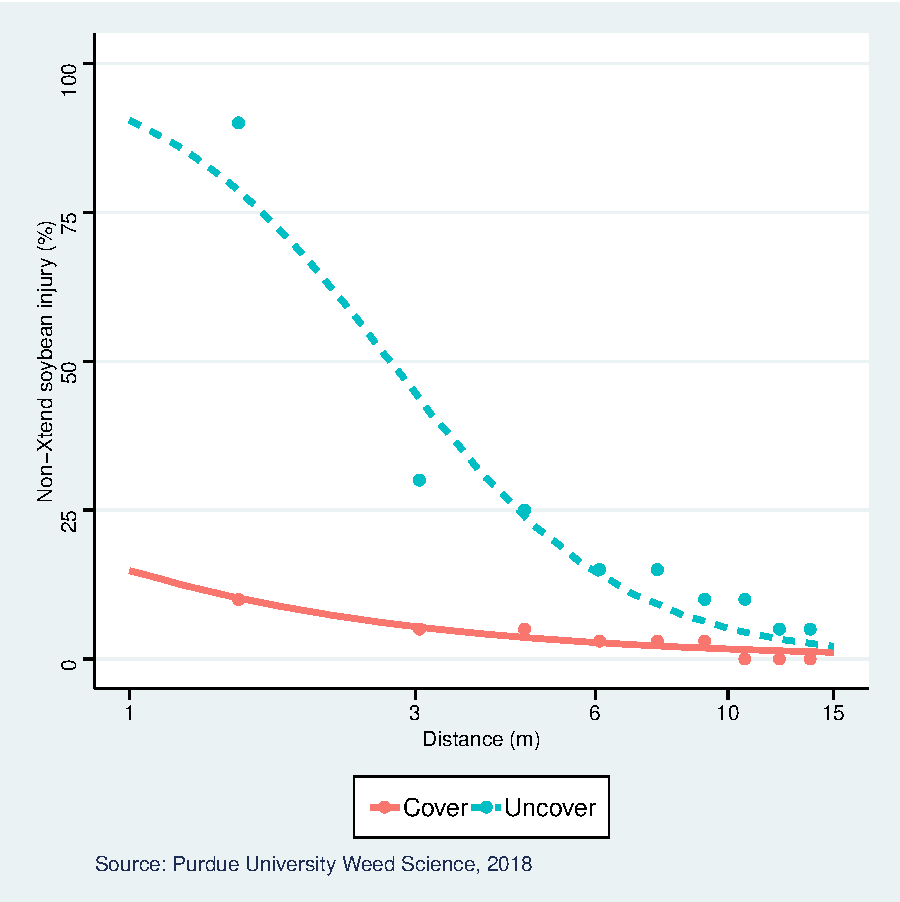
\includegraphics{Report_Dicamba_study_files/figure-latex/unnamed-chunk-27-1.pdf}
\caption{Non-Xtend soybean injury (\%) with distance (\%) from the
dicamba treated area of north (cover and uncover) at 21 DAT in Indiana.}
\end{figure}

\newpage

\paragraph{\texorpdfstring{Area located in the \textbf{Middle} (cover
and
uncover)}{Area located in the Middle (cover and uncover)}}\label{area-located-in-the-middle-cover-and-uncover}

\begin{longtable}[]{@{}lllll@{}}
\caption{Parameters of the log-logistic model of middle (cover and
uncover) at 21 DAT in Indiana.}\tabularnewline
\toprule
Parameter & Area & Estimate (± SE) & t-value & p-value\tabularnewline
\midrule
\endfirsthead
\toprule
Parameter & Area & Estimate (± SE) & t-value & p-value\tabularnewline
\midrule
\endhead
Slope & Cover & 1.38 ± 0.98 & 1.39 & 0.18\tabularnewline
Slope & Uncover & 2.24 ± 0.28 & 7.76 & 0.00 ***\tabularnewline
Asymptote & Cover & 100 & &\tabularnewline
Asymptote & Uncover & 100 & &\tabularnewline
ED50 & Cover & 0.31 ± 0.42 & 0.74 & 0.46\tabularnewline
ED50 & Uncover & 2.71 ± 0.17 & 15.71 & 0.00 ***\tabularnewline
\bottomrule
\end{longtable}

\begin{longtable}[]{@{}llll@{}}
\caption{Estimation of the distance (m) that resulted in 1 (ED1), 10
(ED10), and 20\% (ED20) injury on non-Xtend soybeans of middle (cover
and uncover) at 21 DAT in Indiana.}\tabularnewline
\toprule
Area & ED1 (m) (± SE) & ED10 (m) (± SE) & ED20 (m) (± SE)\tabularnewline
\midrule
\endfirsthead
\toprule
Area & ED1 (m) (± SE) & ED10 (m) (± SE) & ED20 (m) (± SE)\tabularnewline
\midrule
\endhead
Cover & 8.83 ± 10.1 & 1.55 ± 0.62 & 0.86 ± 0.59\tabularnewline
Uncover & 21.1 ± 5.41 & 7.23 ± 0.92 & 5.03 ± 0.45\tabularnewline
\bottomrule
\end{longtable}

\begin{longtable}[]{@{}llll@{}}
\caption{Comparison of EDs among four sides of middle (cover and
uncover) at 21 DAT in Indiana.}\tabularnewline
\toprule
Comparison & Estimate (± SE) & t-value & p-value\tabularnewline
\midrule
\endfirsthead
\toprule
Comparison & Estimate (± SE) & t-value & p-value\tabularnewline
\midrule
\endhead
Cover/Uncover:ED1/ED1 & 0.41 ± 0.49 & -1.18 & 0.25\tabularnewline
Cover/Uncover:ED10/ED10 & 0.21 ± 0.09 & -8.64 & 0.00\tabularnewline
Cover/Uncover:ED20/ED20 & 0.17 ± 0.11 & -6.95 & 0.00\tabularnewline
\bottomrule
\end{longtable}

\begin{figure}
\centering
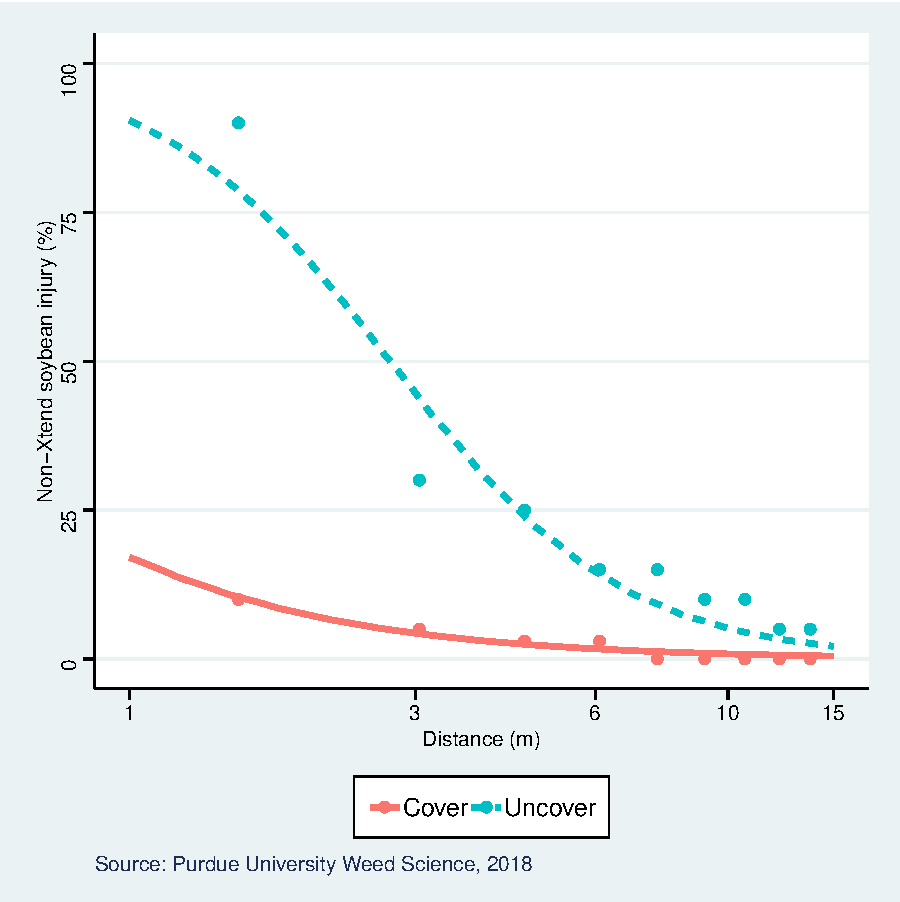
\includegraphics{Report_Dicamba_study_files/figure-latex/unnamed-chunk-30-1.pdf}
\caption{Non-Xtend soybean injury (\%) with distance (\%) from the
dicamba treated area of middle (cover and uncover) at 21 DAT in
Indiana.}
\end{figure}

\newpage

\paragraph{\texorpdfstring{Area located in the \textbf{South} (cover and
uncover)}{Area located in the South (cover and uncover)}}\label{area-located-in-the-south-cover-and-uncover}

\begin{longtable}[]{@{}lllll@{}}
\caption{Parameters of the log-logistic model of south (cover and
uncover) at 21 DAT in Indiana.}\tabularnewline
\toprule
Parameter & Area & Estimate (± SE) & t-value & p-value\tabularnewline
\midrule
\endfirsthead
\toprule
Parameter & Area & Estimate (± SE) & t-value & p-value\tabularnewline
\midrule
\endhead
Slope & Cover & 5.01 ± 36.04 & 0.13 & 0.89\tabularnewline
Slope & Uncover & 2.86 ± 0.31 & 9.19 & 0.00 ***\tabularnewline
Asymptote & Cover & 100 & &\tabularnewline
Asymptote & Uncover & 100 & &\tabularnewline
ED50 & Cover & 0.75 ± 3.80 & 0.19 & 0.84\tabularnewline
ED50 & Uncover & 2.42 ± 0.10 & 23.6 & 0.00 ***\tabularnewline
\bottomrule
\end{longtable}

\begin{longtable}[]{@{}llll@{}}
\caption{Estimation of the distance (m) that resulted in 1 (ED1), 10
(ED10), and 20\% (ED20) injury on non-Xtend soybeans of south (cover and
uncover) at 21 DAT in Indiana.}\tabularnewline
\toprule
Area & ED1 (m) (± SE) & ED10 (m) (± SE) & ED20 (m) (± SE)\tabularnewline
\midrule
\endfirsthead
\toprule
Area & ED1 (m) (± SE) & ED10 (m) (± SE) & ED20 (m) (± SE)\tabularnewline
\midrule
\endhead
Cover & 1.90 ± 3.07 & 1.17 ± 2.19 & 1.00 ± 3.02\tabularnewline
Uncover & 12.0 ± 2.08 & 5.22 ± 0.45 & 3.93 ± 0.24\tabularnewline
\bottomrule
\end{longtable}

\begin{longtable}[]{@{}llll@{}}
\caption{Comparison of EDs among four sides of south (cover and uncover)
at 21 DAT in Indiana.}\tabularnewline
\toprule
Comparison & Estimate (± SE) & t-value & p-value\tabularnewline
\midrule
\endfirsthead
\toprule
Comparison & Estimate (± SE) & t-value & p-value\tabularnewline
\midrule
\endhead
Cover/Uncover:ED1/ED1 & 0.15 ± 0.25 & -3.28 & 0.00\tabularnewline
Cover/Uncover:ED10/ED10 & 0.22 ± 0.42 & -1.84 & 0.08\tabularnewline
Cover/Uncover:ED20/ED20 & 0.25 ± 0.76 & -0.96 & 0.34\tabularnewline
\bottomrule
\end{longtable}

\begin{figure}
\centering
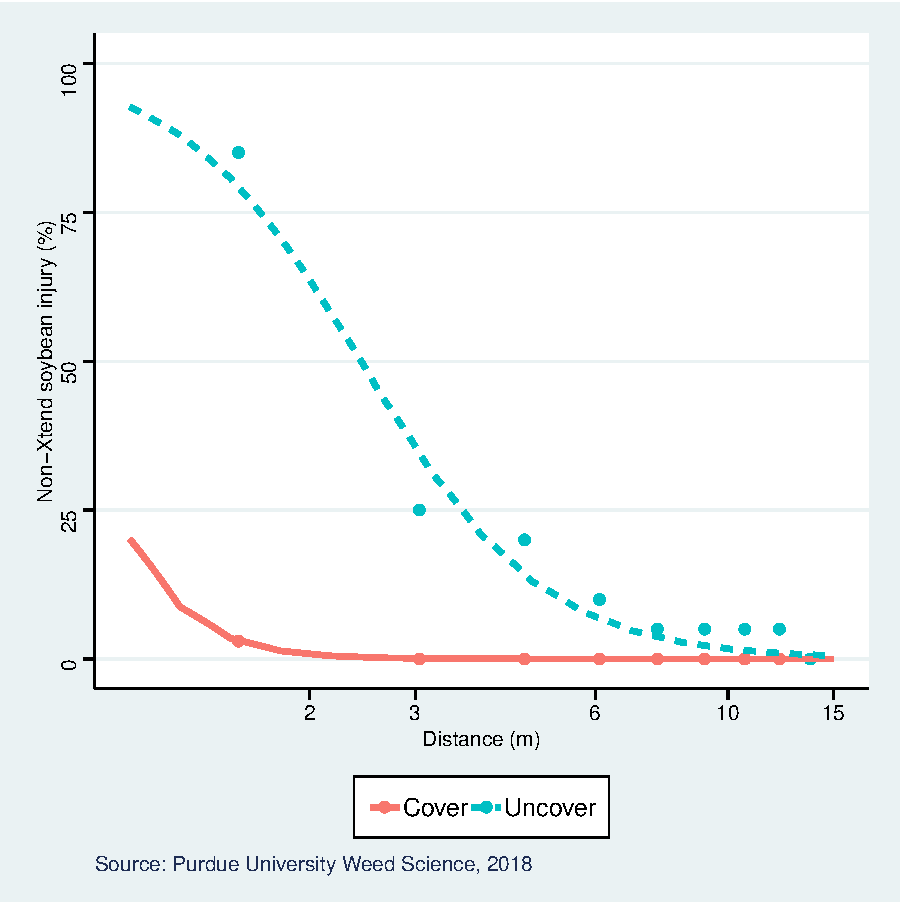
\includegraphics{Report_Dicamba_study_files/figure-latex/IN21S2Plot-1.pdf}
\caption{Non-Xtend soybean injury (\%) with distance (\%) from the
dicamba treated area of south (cover and uncover) at 21 DAT in Indiana.}
\end{figure}

\newpage

\paragraph{\texorpdfstring{Area located in the \textbf{Transects}
(north, middle, ans
south)}{Area located in the Transects (north, middle, ans south)}}\label{area-located-in-the-transects-north-middle-ans-south}

\begin{longtable}[]{@{}lllll@{}}
\caption{Parameters of the log-logistic model of transect north, middle,
and south at 21 DAT in Indiana.}\tabularnewline
\toprule
Parameter & Transect & Estimate (± SE) & t-value &
p-value\tabularnewline
\midrule
\endfirsthead
\toprule
Parameter & Transect & Estimate (± SE) & t-value &
p-value\tabularnewline
\midrule
\endhead
Slope & north & 1.18 ± 0.15 & 7.47 & 0.00 ***\tabularnewline
Slope & Middle & 5.00 ± 2.72 & 1.83 & 0.08 .\tabularnewline
Slope & South & 1.20 ± 0.32 & 3.69 & 0.01 ***\tabularnewline
Asymptote & north & 100 & &\tabularnewline
Asymptote & Middle & 100 & &\tabularnewline
Asymptote & South & 100 & &\tabularnewline
ED50 & north & 1.61 ± 0.29 & 5.54 & 0.00 ***\tabularnewline
ED50 & Middle & 3.34 ± 0.32 & 10.43 & 0.00 ***\tabularnewline
ED50 & South & 0.91 ± 0.43 & 2.09 & 0.05 .\tabularnewline
\bottomrule
\end{longtable}

\begin{longtable}[]{@{}llll@{}}
\caption{Estimation of the distance (m) that resulted in 1 (ED1), 10
(ED10), and 20\% (ED20) injury on non-Xtend soybeans of transect north,
middle, and south at 21 DAT in Indiana.}\tabularnewline
\toprule
Transect & ED1 (m) (± SE) & ED10 (m) (± SE) & ED20 (m) (±
SE)\tabularnewline
\midrule
\endfirsthead
\toprule
Transect & ED1 (m) (± SE) & ED10 (m) (± SE) & ED20 (m) (±
SE)\tabularnewline
\midrule
\endhead
North & 78.0 ± 28.36 & 10.31 ± 1.17 & 5.20 ± 0.39\tabularnewline
Middle & 8.36 ± 3.40 & 5.18 ± 0.76 & 4.41 ± 0.26\tabularnewline
South & 41.5 ± 24.3 & 5.64 ± 0.71 & 2.87 ± 0.55\tabularnewline
\bottomrule
\end{longtable}

\begin{longtable}[]{@{}llll@{}}
\caption{Comparison of EDs among four sides of transect north, middle,
and south at 21 DAT in Indiana.}\tabularnewline
\toprule
Comparison & Estimate (± SE) & t-value & p-value\tabularnewline
\midrule
\endfirsthead
\toprule
Comparison & Estimate (± SE) & t-value & p-value\tabularnewline
\midrule
\endhead
Middle/North:ED1/ED1 & 0.11 ± 0.05 & -1.52 & 0.00\tabularnewline
Middle/South:ED1/ED1 & 0.20 ± 0.14 & -5.54 & 0.00\tabularnewline
North/South:ED1/ED1 & 1.88 ± 1.29 & 0.67 & 0.50\tabularnewline
Middle/North:ED10/ED10 & 0.50 ± 0.09 & -5.31 & 0.00\tabularnewline
Middle/South:ED10/ED10 & 0.94 ± 0.17 & 0.45 & 0.65\tabularnewline
North/South:ED10/ED10 & -0.91 ± -0.18 & -0.45 & 0.65\tabularnewline
Middle/North:ED20/ED20 & -0.84 ± -0.08 & -1.83 & 0.08\tabularnewline
Middle/South:ED20/ED20 & 1.53 ± 0.31 & 1.72 & 0.10\tabularnewline
North/South:ED20/ED20 & 1.81 ± 0.37 & 2.15 & 0.04\tabularnewline
\bottomrule
\end{longtable}

\begin{figure}
\centering
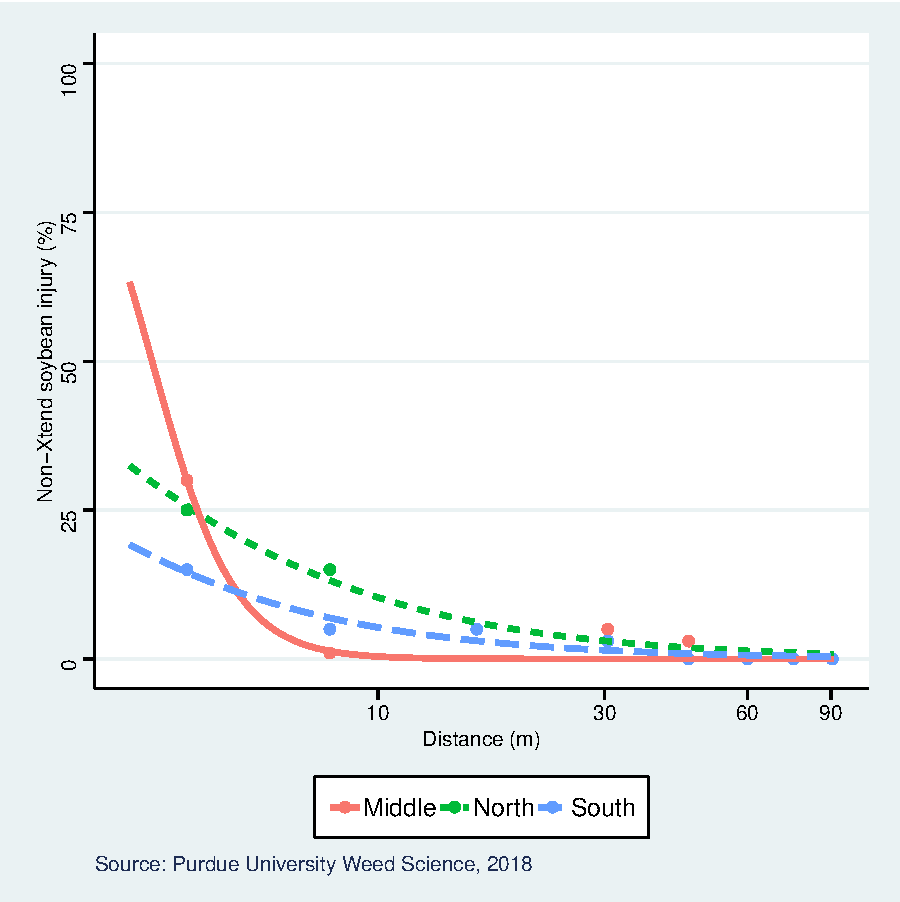
\includegraphics{Report_Dicamba_study_files/figure-latex/unnamed-chunk-34-1.pdf}
\caption{Non-Xtend soybean injury (\%) with distance (\%) from the
dicamba treated area of transect (north, middle, and south) at 21 DAT in
Indiana.}
\end{figure}

\newpage

\pagebreak

\subsubsection{Non-Xtend soybeans
height}\label{non-xtend-soybeans-height-2}

\paragraph{\texorpdfstring{Area located in the \textbf{North} direction
(cover and
uncover)}{Area located in the North direction (cover and uncover)}}\label{area-located-in-the-north-direction-cover-and-uncover-1}

\begin{figure}
\centering
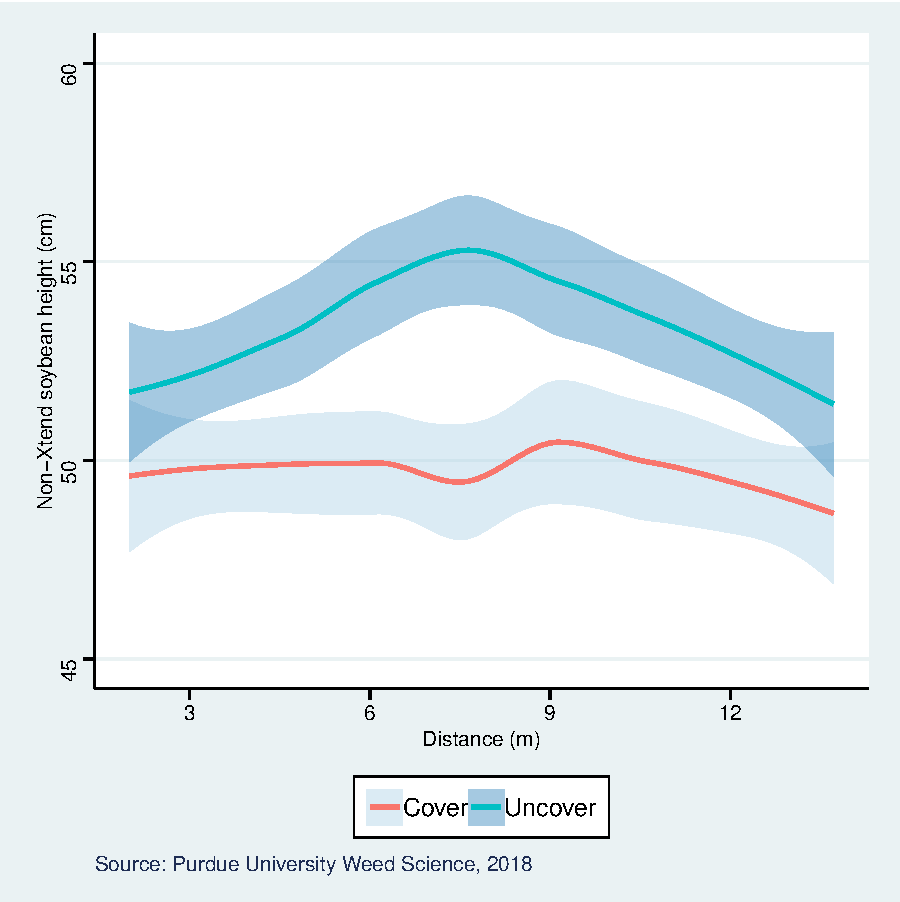
\includegraphics{Report_Dicamba_study_files/figure-latex/unnamed-chunk-36-1.pdf}
\caption{Non-Xtend soybean height (cm) with distance (\%) from the
dicamba treated area of north (cover and uncover) at 21 DAT in Indiana.}
\end{figure}

\pagebreak
\newpage

\paragraph{\texorpdfstring{Area located in the \textbf{Middle} direction
(cover and
uncover)}{Area located in the Middle direction (cover and uncover)}}\label{area-located-in-the-middle-direction-cover-and-uncover}

\begin{figure}
\centering
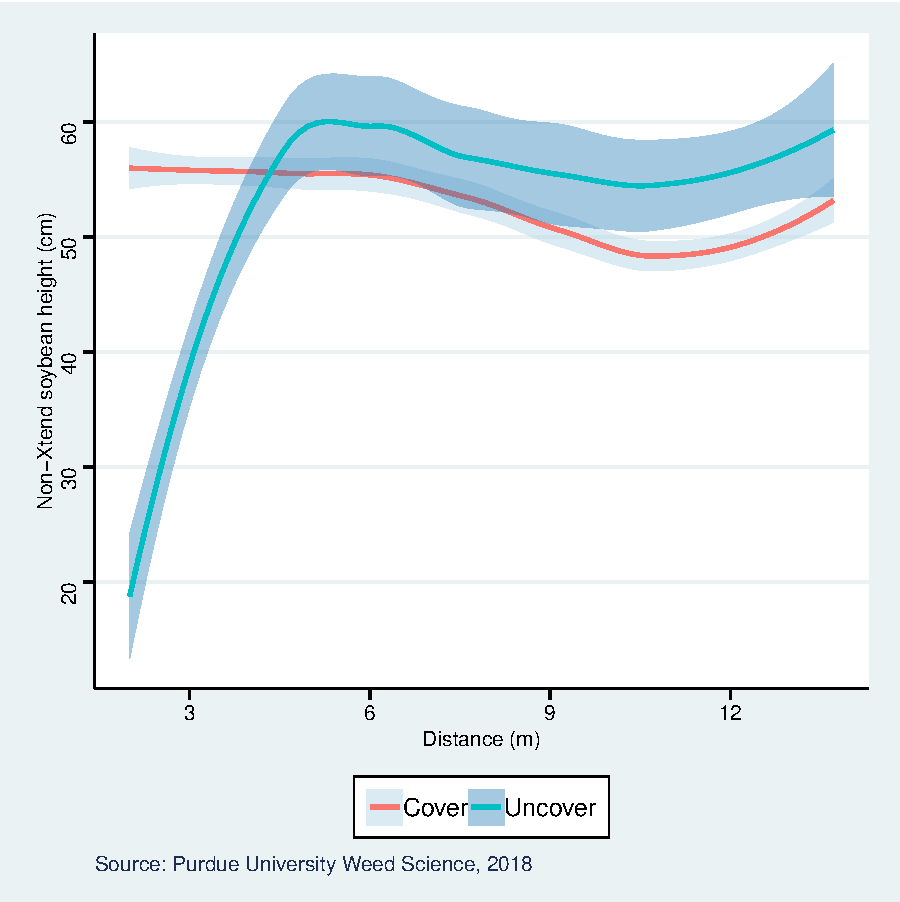
\includegraphics{Report_Dicamba_study_files/figure-latex/unnamed-chunk-37-1.pdf}
\caption{Non-Xtend soybean height (cm) with distance (\%) from the
dicamba treated area of middle (cover and uncover) at 21 DAT in
Indiana.}
\end{figure}

\newpage

\paragraph{\texorpdfstring{Area located in the \textbf{South} direction
(cover and
uncover)}{Area located in the South direction (cover and uncover)}}\label{area-located-in-the-south-direction-cover-and-uncover}

\begin{figure}
\centering
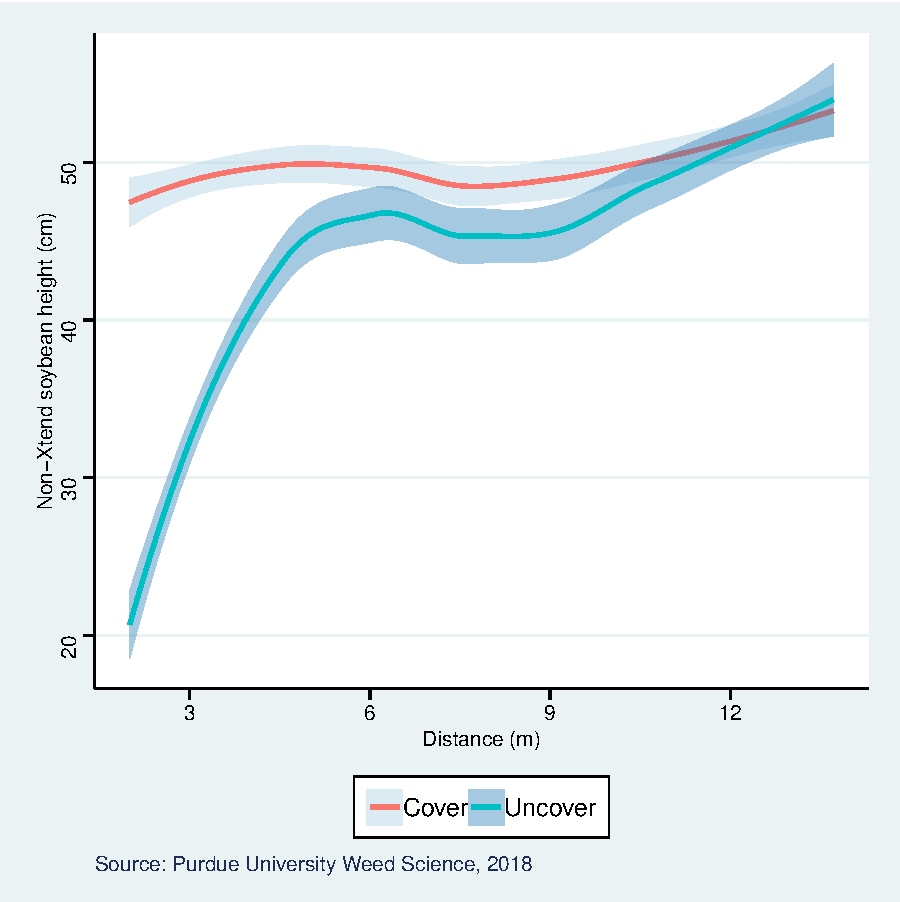
\includegraphics{Report_Dicamba_study_files/figure-latex/unnamed-chunk-38-1.pdf}
\caption{Non-Xtend soybean height (cm) with distance (\%) from the
dicamba treated area of middle (cover and uncover) at 21 DAT in
Indiana.}
\end{figure}

\pagebreak
\newpage

\paragraph{\texorpdfstring{Area located in the \textbf{Transects}
(north, middle, and
south)}{Area located in the Transects (north, middle, and south)}}\label{area-located-in-the-transects-north-middle-and-south}

\begin{figure}
\centering
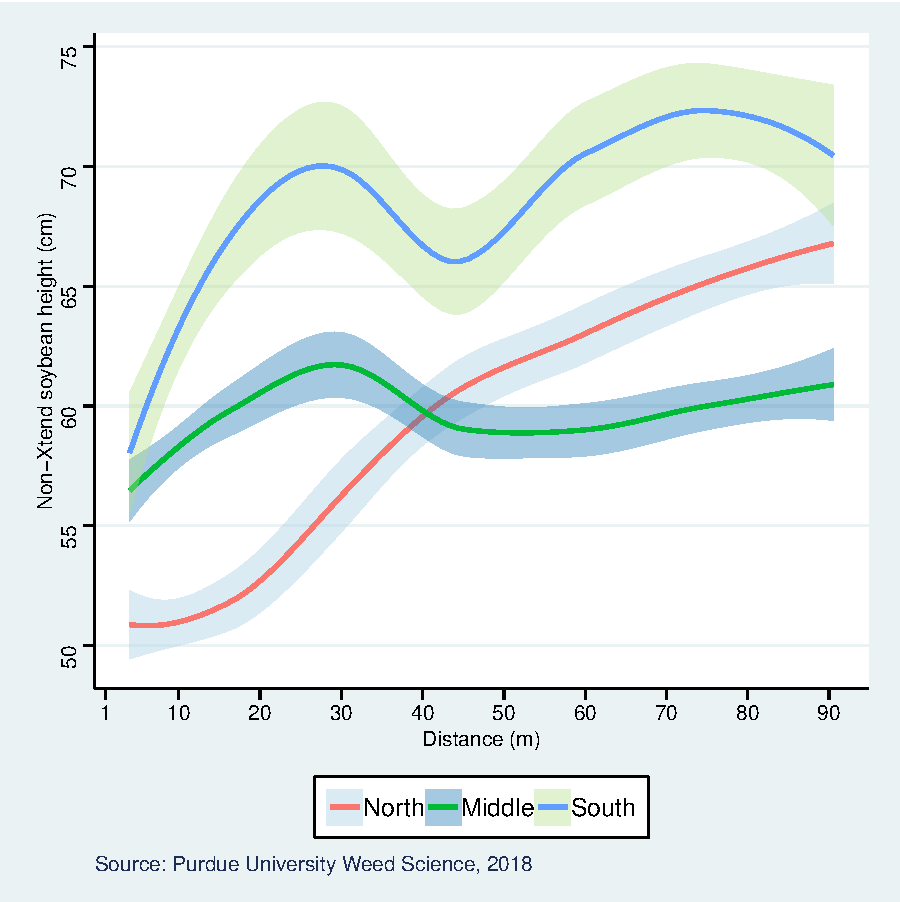
\includegraphics{Report_Dicamba_study_files/figure-latex/unnamed-chunk-39-1.pdf}
\caption{Non-Xtend soybean height (cm) with distance (\%) from the
dicamba treated area of transect north, middle, and south at 21 DAT in
Indiana.}
\end{figure}

\pagebreak

\section{MICHIGAN}\label{michigan-1}

\subsection{Location}\label{location-2}

The study was conducted in 53 of a 300 acre field at Van Gilder Farms
Fowlerville, Michigan (Figure 12).

\begin{figure}[h]

{\centering \includegraphics[width=1\linewidth]{Michigan} 

}

\caption{Aerial view of the large scale volatility trial in Michigan.}\label{fig:unnamed-chunk-40}
\end{figure}

\pagebreak

\subsection{Modeling}\label{modeling-2}

Non-Xtend \textbf{soybean injury (\%)} (visual data) from Michigan
presented here was collected in from one soybean plant
distance\textsuperscript{-1} at 21 DAT but without replication.
Nonetheless, we use the three-parameter logistic model (Equation 1) for
fitting soybean injury (\%) with distance from the area treated with
dicamba.

Equation 1: \[Y= \frac{d}{(1 + exp[b(logx - loge)]} \]

where \emph{Y} is the soybean injury (\%), \emph{x} is the distance (m)
from the dicamba treated area. in The parameter \emph{d} is the upper
limit (asymptote), \emph{b} is the slope and the parameter \emph{e} is
the ED50 (effective \emph{x} that causes 50\% reduction in \emph{Y}).
The upper limit of the model is locked at 100. Only data recorded 21 DAT
is presented.

Non-Xtend \textbf{soybean height} (cm) from Michigan presented here was
collected from 10 soybean plant distance\textsuperscript{-1} at 21 DAT.
\emph{Loess} local regression was fitted to the data.

\pagebreak
\newpage

\subsection{Wind}\label{wind-2}

Frequency of wind direction and speed (m/s) three days after dicamaba
application (Figure X).

\begin{figure}
\centering
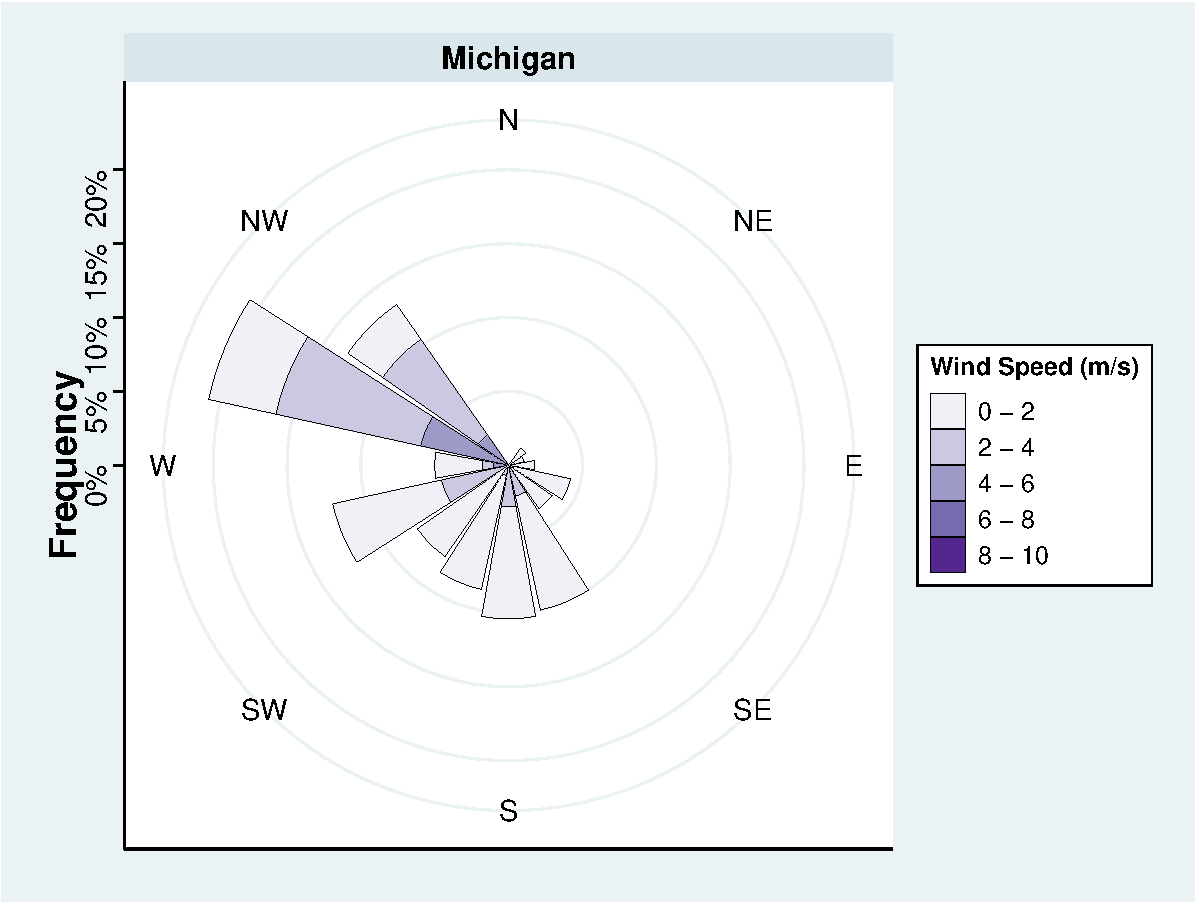
\includegraphics{Report_Dicamba_study_files/figure-latex/unnamed-chunk-43-1.pdf}
\caption{Wind rose plots demonstrating the average wind frequency (\%)
and wind speed (m s\textsuperscript{1}) grouped in 22.5° of direction
(from which the wind is blowing) in Michigan.}
\end{figure}

\pagebreak
\newpage

\subsection{Transects}\label{transects-2}

\begin{figure}[h]

{\centering 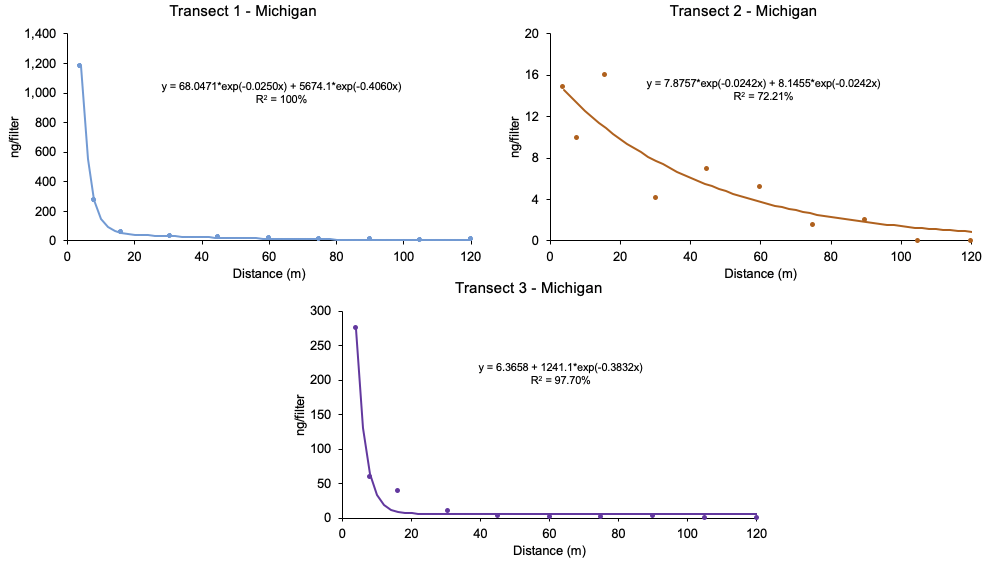
\includegraphics[width=1\linewidth]{MItransect} 

}

\caption{Deposition of dicamba particles at the transects in Michigan}\label{fig:unnamed-chunk-44}
\end{figure}

\pagebreak
\newpage

\newpage

\pagebreak

\subsection{Results at 21 DAT}\label{results-at-21-dat-1}

\subsubsection{Dicamba injury (\%) in non-Xtend
soybeans}\label{dicamba-injury-in-non-xtend-soybeans-3}

\paragraph{Area located at downwind A (cover and
uncover)}\label{area-located-at-downwind-a-cover-and-uncover}

\begin{longtable}[]{@{}lllll@{}}
\caption{Parameters of the log-logistic model at area A (cover and
uncover) at 21 DAT in Michigan.}\tabularnewline
\toprule
Parameter & Area & Estimate (± SE) & t-value & p-value\tabularnewline
\midrule
\endfirsthead
\toprule
Parameter & Area & Estimate (± SE) & t-value & p-value\tabularnewline
\midrule
\endhead
Slope & Cover & 1.41 ± 0.66 & 2.11 & 0.04185 *\tabularnewline
Slope & Uncover & 2.55 ± 0.22 & 11.53 & 0.00 ***\tabularnewline
Asymptote & Cover & 14.96 ± 2.46 & 6.08 & 0.00 ***\tabularnewline
Asymptote & Uncover & 59.63 ± 1.22 & 48.68 & 0.00 ***\tabularnewline
ED50 & Cover & 0.54 ± 0.33 & 1.63 & 0.11\tabularnewline
ED50 & Uncover & 10.73 ± 0.29 & 36.65 & 0.00 ***\tabularnewline
\bottomrule
\end{longtable}

\begin{longtable}[]{@{}llll@{}}
\caption{Estimation of the distance (m) that resulted in 1 (ED1), 10
(ED10), and 20\% (ED20) injury on non-Xtend soybeans at area A (cover
and uncover) at 21 DAT in Michigan.}\tabularnewline
\toprule
Area & ED1 (m) (± SE) & ED10 (m) (± SE) & ED20 (m) (± SE)\tabularnewline
\midrule
\endfirsthead
\toprule
Area & ED1 (m) (± SE) & ED10 (m) (± SE) & ED20 (m) (± SE)\tabularnewline
\midrule
\endhead
Uncover & 52.86 ± 6.93 & 20.10 ± 1.03 & 14.03 ± 0.40\tabularnewline
Cover & 3.52 ± 2.05 & 0.32 ± 0.26 & NA\tabularnewline
\bottomrule
\end{longtable}

\begin{longtable}[]{@{}llll@{}}
\caption{Comparison of EDs between UNcover and non cover areas in
non-Xtend soybeans at area A (cover and uncover) at 21 DAT in
Michigan.}\tabularnewline
\toprule
Comparison & Estimate (± SE) & t-value & p-value\tabularnewline
\midrule
\endfirsthead
\toprule
Comparison & Estimate (± SE) & t-value & p-value\tabularnewline
\midrule
\endhead
Uncover/Cover:ED1/ED1 & 14.97 ± 8.94 & 1.51 & 0.12\tabularnewline
Uncover/Cover:ED10/ED10 & 60.93 ± 49.07 & 1.22 & 0.22\tabularnewline
Uncover/Cover:ED20/ED20 & NA & NA & NA\tabularnewline
\bottomrule
\end{longtable}

\begin{figure}
\centering
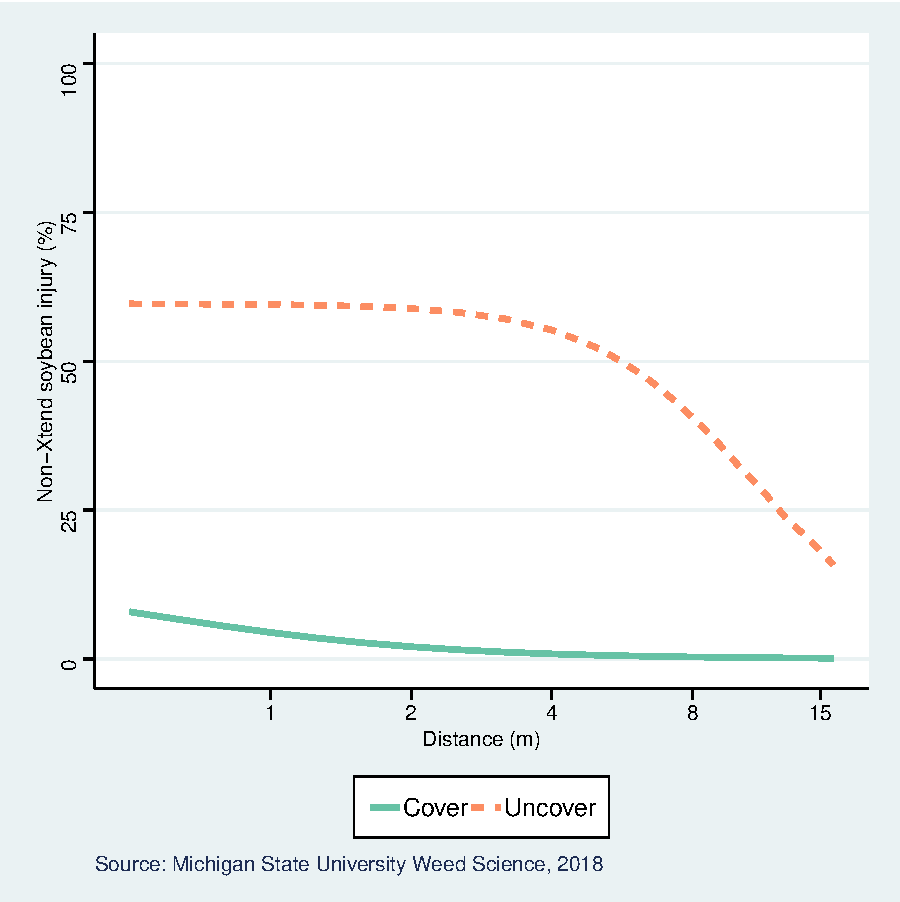
\includegraphics{Report_Dicamba_study_files/figure-latex/unnamed-chunk-47-1.pdf}
\caption{Non-Xtend soybean injury (\%) with distance (\%) from the
dicamba treated at A (cover and uncover) at 21 DAT in Michigan.}
\end{figure}

\pagebreak

\paragraph{Area located at downwind B (cover and
uncover)}\label{area-located-at-downwind-b-cover-and-uncover}

\begin{longtable}[]{@{}lllll@{}}
\caption{Parameters of the log-logistic model at area B (cover and
uncover) at 21 DAT in Michigan.}\tabularnewline
\toprule
Parameter & Area & Estimate (± SE) & t-value & p-value\tabularnewline
\midrule
\endfirsthead
\toprule
Parameter & Area & Estimate (± SE) & t-value & p-value\tabularnewline
\midrule
\endhead
Slope & Cover & 2.27 ± 0.26 & 8.65 & 0.00 ***\tabularnewline
Slope & Uncover & 1.60 ± 0.14 & 11.32 & 0.00 ***\tabularnewline
Asymptote & Cover & 14.91 ± 0.87 & 17.12 & 0.00 ***\tabularnewline
Asymptote & Uncover & 19.83 ± 0.96 & 20.64 & 0.00 ***\tabularnewline
ED50 & Cover & 2.59 ± 0.26 & 9.94 & 0.00 ***\tabularnewline
ED50 & Uncover & 1.78 ± 0.18 & 10.01 & 0.00 ***\tabularnewline
\bottomrule
\end{longtable}

\begin{longtable}[]{@{}llll@{}}
\caption{Estimation of the distance (m) that resulted in 1 (ED1), 10
(ED10), and 20\% (ED20) injury on non-Xtend soybeans at area B (cover
and uncover) at 21 DAT in Michigan.}\tabularnewline
\toprule
Area & ED1 (m) (± SE) & ED10 (m) (± SE) & ED20 (m) (± SE)\tabularnewline
\midrule
\endfirsthead
\toprule
Area & ED1 (m) (± SE) & ED10 (m) (± SE) & ED20 (m) (± SE)\tabularnewline
\midrule
\endhead
Uncover & 11.13 ± 1.36 & 1.76 ± 0.17 & NA\tabularnewline
Cover & 8.25 ± 0.81 & 1.89 ± 0.24 & NA\tabularnewline
\bottomrule
\end{longtable}

\begin{longtable}[]{@{}llll@{}}
\caption{Comparison of EDs between uncover and non cover areas in
non-Xtend soybeans at area B (cover and uncover) at 21 DAT in
Michigan.}\tabularnewline
\toprule
Comparison & Estimate (± SE) & t-value & p-value\tabularnewline
\midrule
\endfirsthead
\toprule
Comparison & Estimate (± SE) & t-value & p-value\tabularnewline
\midrule
\endhead
Uncover/Cover:ED1/ED1 & 1.35 ± 0.21 & 1.64 & 0.10\tabularnewline
Uncover/Cover:ED10/ED10 & 0.93 ± 0.15 & -4.43 & 0.66\tabularnewline
Uncover/Cover:ED20/ED20 & NA & NA & NA\tabularnewline
\bottomrule
\end{longtable}

\begin{figure}
\centering
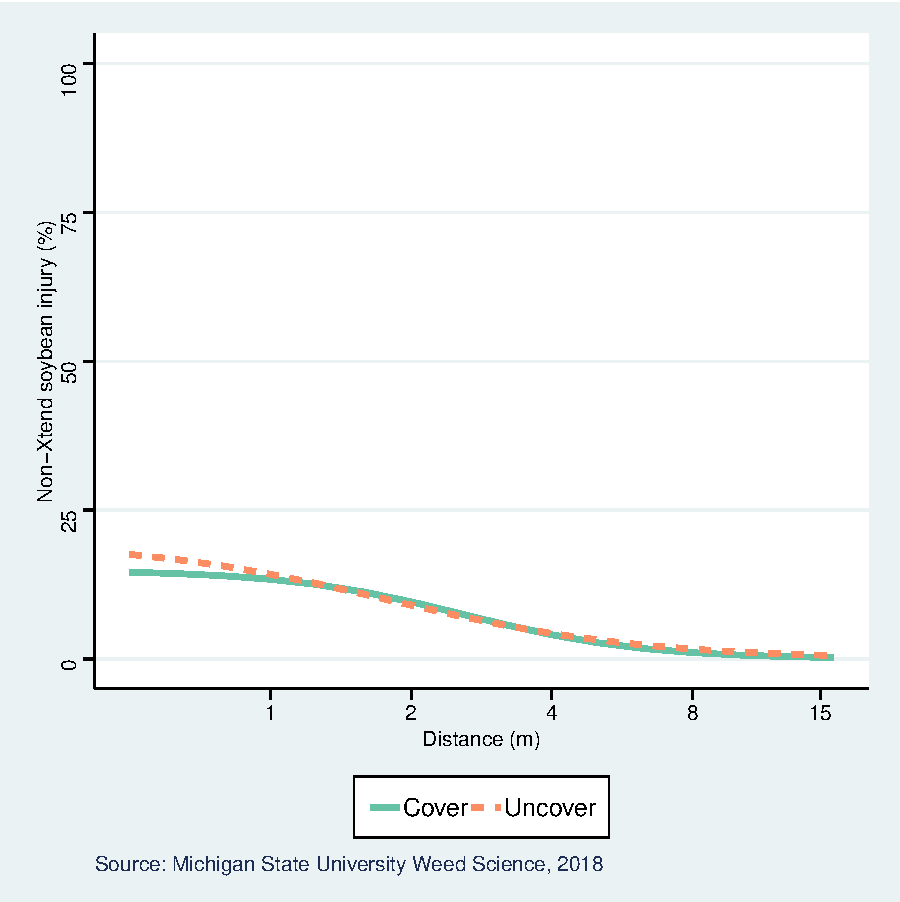
\includegraphics{Report_Dicamba_study_files/figure-latex/unnamed-chunk-50-1.pdf}
\caption{Non-Xtend soybean injury (\%) with distance (\%) from the
dicamba treated area at B (cover and uncover) at 21 DAT in Michigan.}
\end{figure}

\pagebreak

\subsubsection{Area located at downwind C (cover and
uncover)}\label{area-located-at-downwind-c-cover-and-uncover}

\begin{longtable}[]{@{}lllll@{}}
\caption{Parameters of the log-logistic model at area C (cover and
uncover) at 21 DAT in Michigan.}\tabularnewline
\toprule
Parameter & Area & Estimate (± SE) & t-value & p-value\tabularnewline
\midrule
\endfirsthead
\toprule
Parameter & Area & Estimate (± SE) & t-value & p-value\tabularnewline
\midrule
\endhead
Slope & Cover & 2.04 ± 0.71 & 2.89 & 0.00 **\tabularnewline
Slope & Uncover & 2.70 ± 0.34 & 7.87 & 0.00 ***\tabularnewline
Asymptote & Cover & 9.64 ± 1.73 & 5.55 & 0.00 ***\tabularnewline
Asymptote & Uncover & 35.72 ± 1.73 & 20.66 & 0.00 ***\tabularnewline
ED50 & Cover & 2.79 ± 0.95 & 2.93 & 0.00 **\tabularnewline
ED50 & Uncover & 2.35 ± 0.19 & 12.26 & 0.00 ***\tabularnewline
\bottomrule
\end{longtable}

\begin{longtable}[]{@{}llll@{}}
\caption{Estimation of the distance (m) that resulted in 1 (ED1), 10
(ED10), and 20\% (ED20) injury on non-Xtend soybeans at area C (cover
and uncover) at 21 DAT in Michigan.}\tabularnewline
\toprule
Area & ED1 (m) (± SE) & ED10 (m) (± SE) & ED20 (m) (± SE)\tabularnewline
\midrule
\endfirsthead
\toprule
Area & ED1 (m) (± SE) & ED10 (m) (± SE) & ED20 (m) (± SE)\tabularnewline
\midrule
\endhead
Uncover & 8.76 ± 1.01 & 3.34 ± 0.18 & 2.15 ± 0.19\tabularnewline
Cover & 8.02 ± 1.87 & NA & NA\tabularnewline
\bottomrule
\end{longtable}

\begin{longtable}[]{@{}llll@{}}
\caption{Comparison of EDs between UNcover and non cover areas in
non-Xtend soybeans at area C (cover and uncover) at 21 DAT in
Michigan.}\tabularnewline
\toprule
Comparison & Estimate (± SE) & t-value & p-value\tabularnewline
\midrule
\endfirsthead
\toprule
Comparison & Estimate (± SE) & t-value & p-value\tabularnewline
\midrule
\endhead
Uncover/Cover:ED10/ED10 & 1.09 ± 0.28 & 0.32 & 0.974\tabularnewline
Uncover/Cover:ED10/ED10 & NA & NA & NA\tabularnewline
Uncover/Cover:ED20/ED20 & NA & NA & NA\tabularnewline
\bottomrule
\end{longtable}

\begin{figure}
\centering
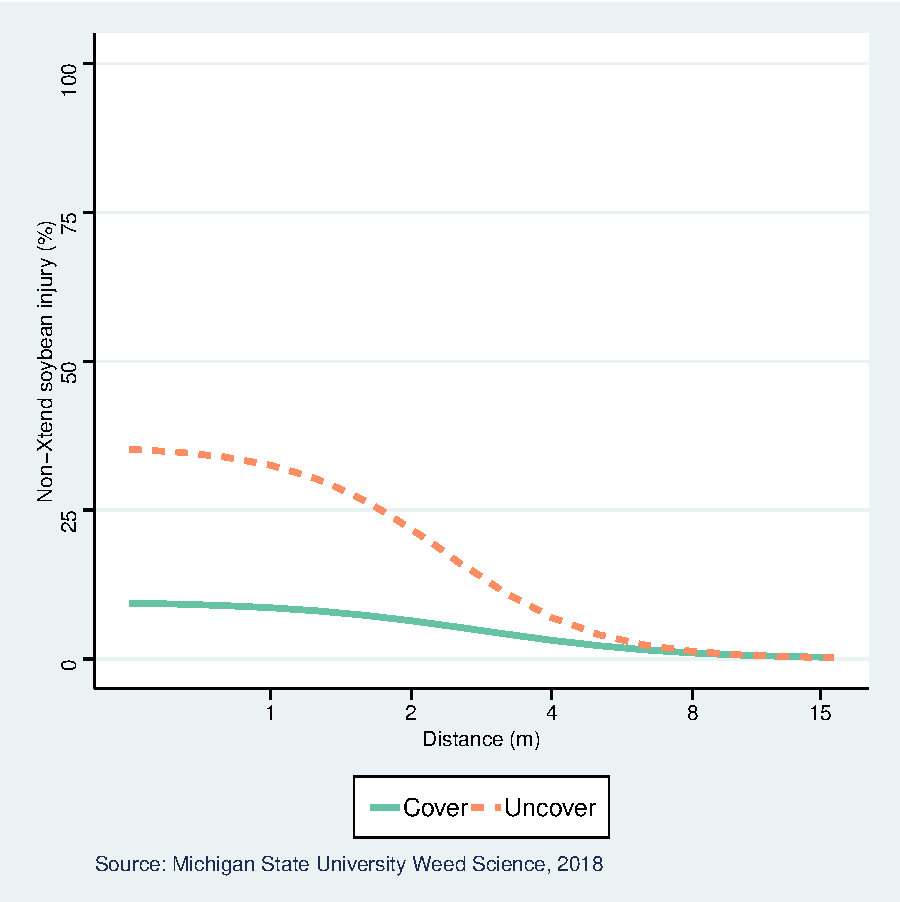
\includegraphics{Report_Dicamba_study_files/figure-latex/unnamed-chunk-53-1.pdf}
\caption{Non-Xtend soybean injury (\%) with distance (\%) from the
dicamba treated area at C (cover and uncover) at 21 DAT in Michigan.}
\end{figure}

\newpage

\pagebreak

\paragraph{\texorpdfstring{Area located in the \textbf{transect} (A, B,
and
C)}{Area located in the transect (A, B, and C)}}\label{area-located-in-the-transect-a-b-and-c}

\begin{longtable}[]{@{}lllll@{}}
\caption{Parameters of the log-logistic model at transect (A, B, and C)
locations at 21 DAT in Michigan.}\tabularnewline
\toprule
Parameter & Transect & Estimate (± SE) & t-value &
p-value\tabularnewline
\midrule
\endfirsthead
\toprule
Parameter & Transect & Estimate (± SE) & t-value &
p-value\tabularnewline
\midrule
\endhead
Slope & A & 6.93 ± 1.65 & 4.19 & 0.00 ***\tabularnewline
Slope & B & 0.69 ± 0.19 & 3.49 & 0.00 **\tabularnewline
Slope & C & 1.27 ± 0.18 & 6.98 & 0.00 ***\tabularnewline
Asymptote & A & 50.84 ± 1.14 & 44.26 & 0.00 ***\tabularnewline
Asymptote & B & 17.75 ± 2.63 & 6.74 & 0.00 ***\tabularnewline
Asymptote & C & 38.25 ± 2.72 & 14.02 & 0.00 ***\tabularnewline
ED50 & A & 10.73 ± 0.82 & 12.93 & 0.00 ***\tabularnewline
ED50 & B & 3.43 ± 1.93 & 1.77 & 0.08 .\tabularnewline
ED50 & C & 5.70 ± 1.14 & 4.96 & 0.00 ***\tabularnewline
\bottomrule
\end{longtable}

\begin{longtable}[]{@{}llll@{}}
\caption{Estimation of the distance (m) that resulted in 1 (ED1), 10
(ED10), and 20\% (ED20) injury on non-Xtend soybeans at transect (A, B,
and C) locations at 21 DAT in Michigan.}\tabularnewline
\toprule
Transect & ED1 (m) (± SE) & ED10 (m) (± SE) & ED20 (m) (±
SE)\tabularnewline
\midrule
\endfirsthead
\toprule
Transect & ED1 (m) (± SE) & ED10 (m) (± SE) & ED20 (m) (±
SE)\tabularnewline
\midrule
\endhead
A & 18.87 ± 3.35 & 13.15 ± 1.38 & 11.42 ± 0.95\tabularnewline
B & 196.98 ± 217.98 & 2.38 ± 1.44 & NA\tabularnewline
C & 98.20 ± 33.82 & 12.90 ± 2.19 & 5.30 ± 1.09\tabularnewline
\bottomrule
\end{longtable}

\begin{longtable}[]{@{}llll@{}}
\caption{Comparison of EDs among transect (A, B, and C) locations at 21
DAT in Michigan.}\tabularnewline
\toprule
Comparison & Estimate (± SE) & t-value & p-value\tabularnewline
\midrule
\endfirsthead
\toprule
Comparison & Estimate (± SE) & t-value & p-value\tabularnewline
\midrule
\endhead
A/B:E1/E1 & 0.09 ± 0.10 & -8.42 & 0.00\tabularnewline
A/C:E1/E1 & 0.19 ± 0.07 & -1.08 & 0.00\tabularnewline
B/C:E1/E1 & 2.00 ± 2.32 & 0.43 & 0.66\tabularnewline
A/B:E10/E10 & 5.51 ± 3.38 & 1.33 & 0.19\tabularnewline
A/C:E10/E10 & 1.01 ± 0.20 & 0.09 & 0.92\tabularnewline
B/C:E10/E10 & 0.18 ± 0.11 & -7.01 & 0.00\tabularnewline
A/B:E20/E20 & NA & NA & NA\tabularnewline
A/C:E20/E20 & 2.15 ± 0.48 & 0.02 & 0.00\tabularnewline
B/C:E20/E20 & NA & NA & NA\tabularnewline
\bottomrule
\end{longtable}

\begin{figure}
\centering
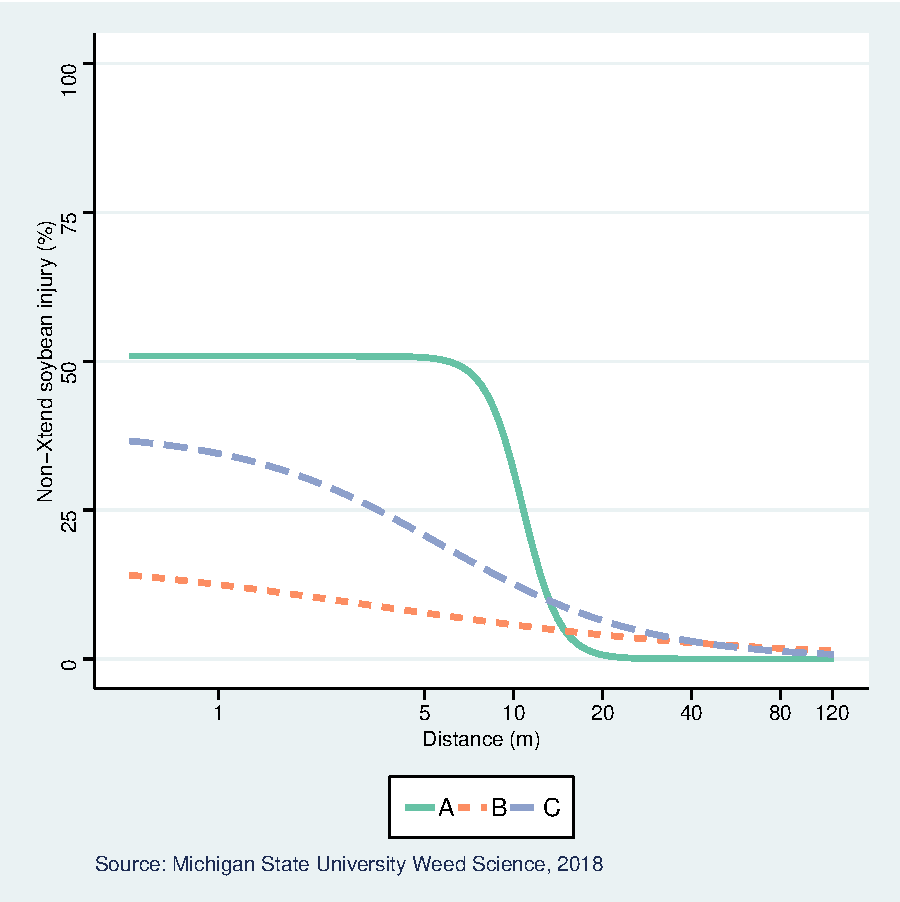
\includegraphics{Report_Dicamba_study_files/figure-latex/unnamed-chunk-56-1.pdf}
\caption{Non-Xtend soybean injury (\%) with distance (\%) from the
dicamba treated area in the at transect (A, B, and C) locations at 21
DAT in Michigan.}
\end{figure}

\newpgae
\pagebreak

\subsubsection{Non-Xtend soybeans
height}\label{non-xtend-soybeans-height-3}

\paragraph{Area located at downwind A (cover and
uncover)}\label{area-located-at-downwind-a-cover-and-uncover-1}

\begin{figure}
\centering
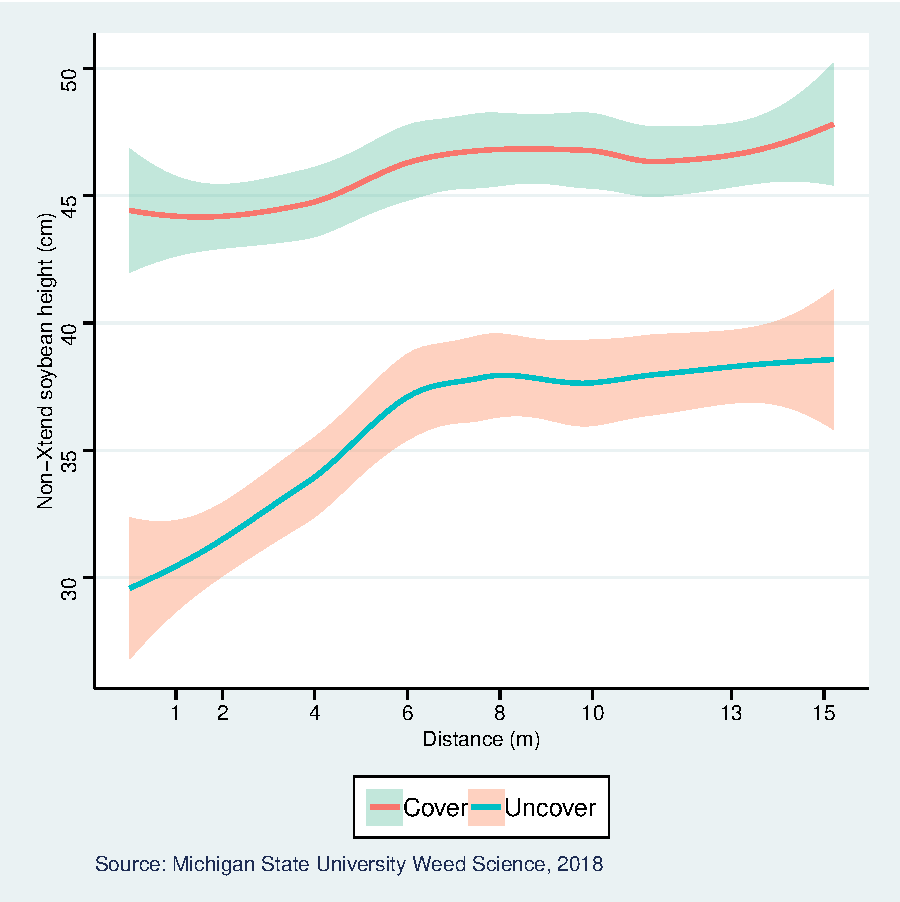
\includegraphics{Report_Dicamba_study_files/figure-latex/unnamed-chunk-57-1.pdf}
\caption{Non-Xtend soybean height (cm) with distance (\%) from the
dicamba treated area in the A location (cover and uncover) at 21 DAT in
Michigan.}
\end{figure}

\newpgae
\pagebreak

\paragraph{Area located at downwind B (cover and
uncover)}\label{area-located-at-downwind-b-cover-and-uncover-1}

\begin{figure}
\centering
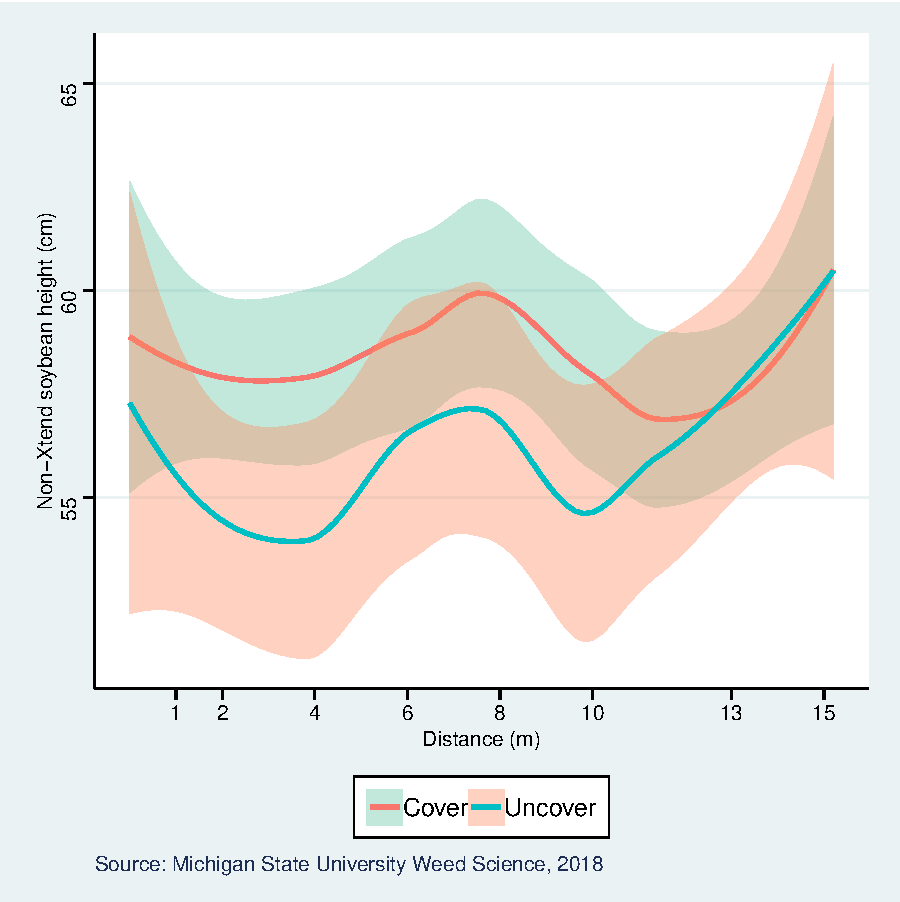
\includegraphics{Report_Dicamba_study_files/figure-latex/unnamed-chunk-58-1.pdf}
\caption{Non-Xtend soybean height (cm) with distance (\%) from the
dicamba treated area in the B location (cover and uncover) at 21 DAT in
Michigan.}
\end{figure}

\newpgae
\pagebreak

\paragraph{Area located at downwind C (cover and
uncover)}\label{area-located-at-downwind-c-cover-and-uncover-1}

\begin{figure}
\centering
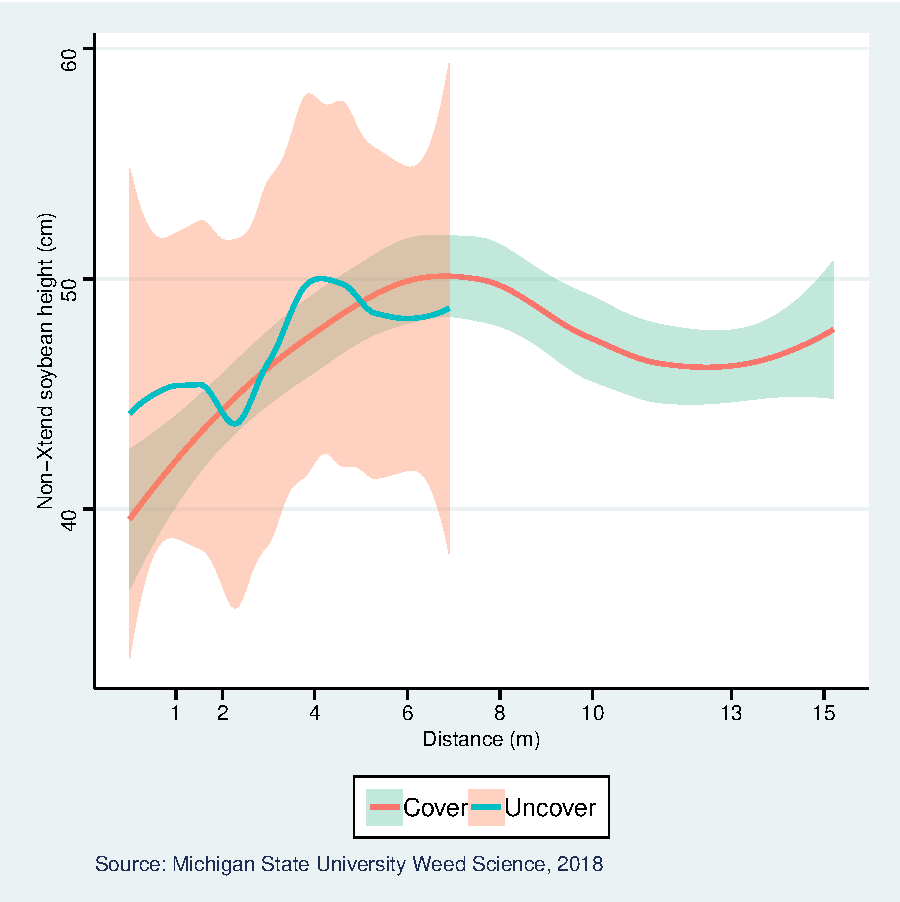
\includegraphics{Report_Dicamba_study_files/figure-latex/unnamed-chunk-59-1.pdf}
\caption{Non-Xtend soybean height (cm) with distance (\%) from the
dicamba treated area in the C location (cover and uncover) at 21 DAT in
Michigan.}
\end{figure}

\newpgae
\pagebreak

\paragraph{\texorpdfstring{Area located in the \textbf{transect} A, B,
and
C}{Area located in the transect A, B, and C}}\label{area-located-in-the-transect-a-b-and-c-1}

\begin{figure}
\centering
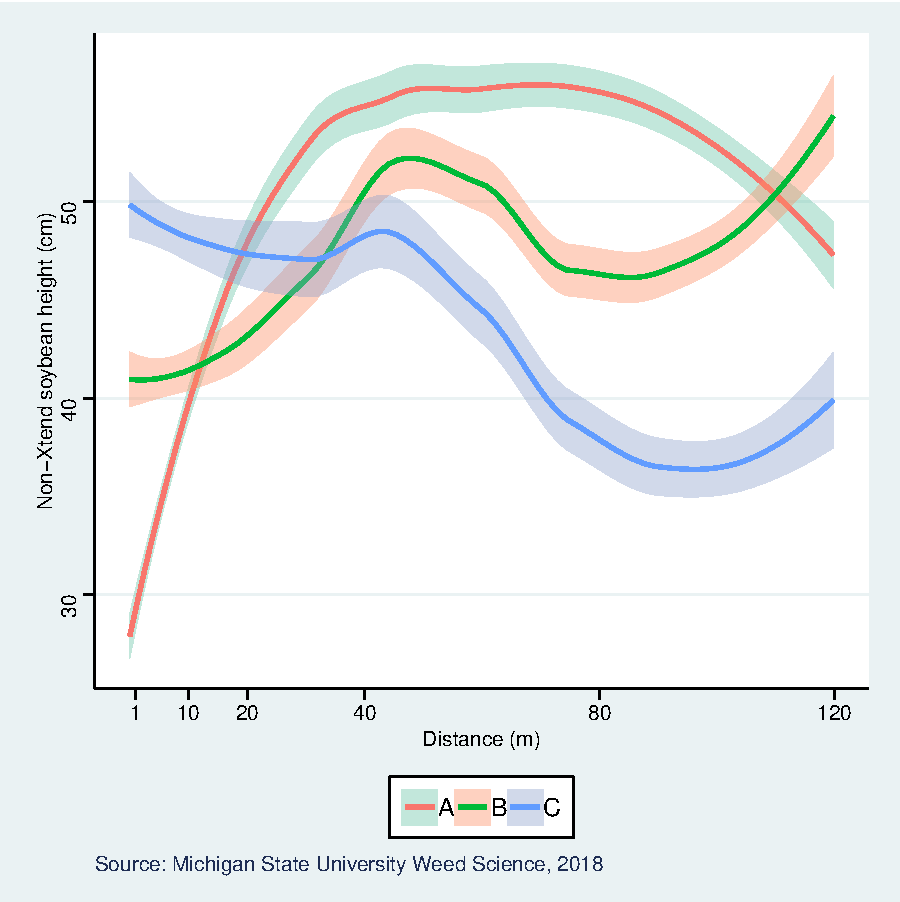
\includegraphics{Report_Dicamba_study_files/figure-latex/unnamed-chunk-60-1.pdf}
\caption{Non-Xtend soybean height (cm) with distance (\%) from the
dicamba treated area in the at transect (A, B, and C) locations at 21
DAT in Michigan.}
\end{figure}

\newpgae
\pagebreak

\section{NEBRASKA}\label{nebraska-1}

\subsection{Location}\label{location-3}

The study was conducted in a soybean field at West Central Research and
Extension of the University of Nebraska-Lincoln (Figure 6).

\begin{figure}[h]

{\centering 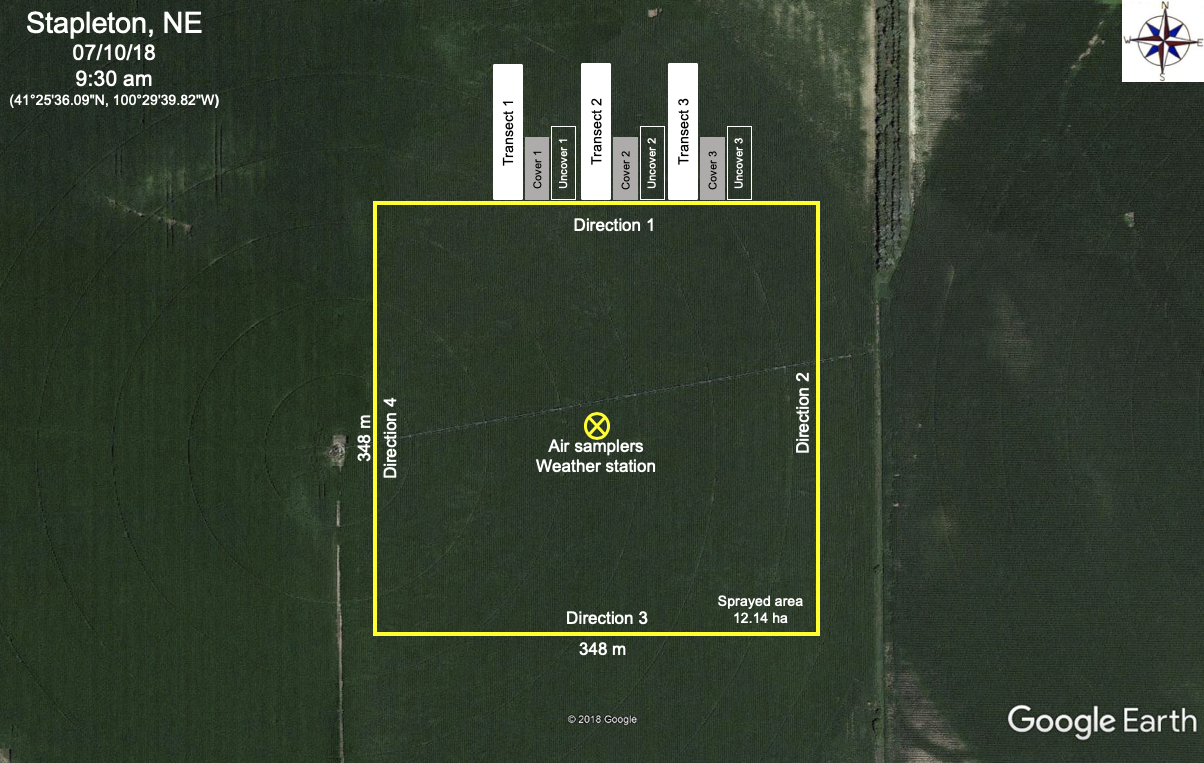
\includegraphics[width=1\linewidth]{nebraska} 

}

\caption{Aerial view of the large scale volatility trial in Nebraska.}\label{fig:unnamed-chunk-61}
\end{figure}

\pagebreak
\newpage

\subsection{Modeling}\label{modeling-3}

Non-Xtend \textbf{soybean injury (\%)} (visual data) from Nebraska
presented here was collected in from one soybean plant
distance\textsuperscript{-1} at 21 DAT but without replication.
Nonetheless, we use the four-parameter logistic model (Equation 2) for
fitting soybean injury (\%) with distance from the area treated with
dicamba.

Equation 2: \[Y= c + \frac{d - c}{(1 + exp[b(logx - loge)]} \]

where \emph{Y} is the soybean injury (\%), \emph{x} is the distance (m)
from the dicamba treated area. in The parameter \emph{d} is the upper
limit (asymptote), \emph{b} is the slope, \emph{c} is the lower limit,
and the parameter \emph{e} is the ED50 (effective \emph{x} that causes
50\% reduction in \emph{Y}).

In some of the Nebraska curves were not possible to estimate the EDs.
Beacuse of estimate values never reached 1, 10, or 20\% non-Xtend
soybean injury, or because the standard error (SE) was higher than the
estimate value.

Non-Xtend \textbf{soybean height} (cm) from Nebraska presented here was
collected from 10 soybean plant distance\textsuperscript{-1} at 21 DAT.
\emph{Loess} local regression was fitted to the data.

\pagebreak
\newpage

\pagebreak
\newpage

\subsection{Wind}\label{wind-3}

Frequency of wind direction and speed (m/s) three days after dicamaba
application (Figure X).

\begin{figure}
\centering
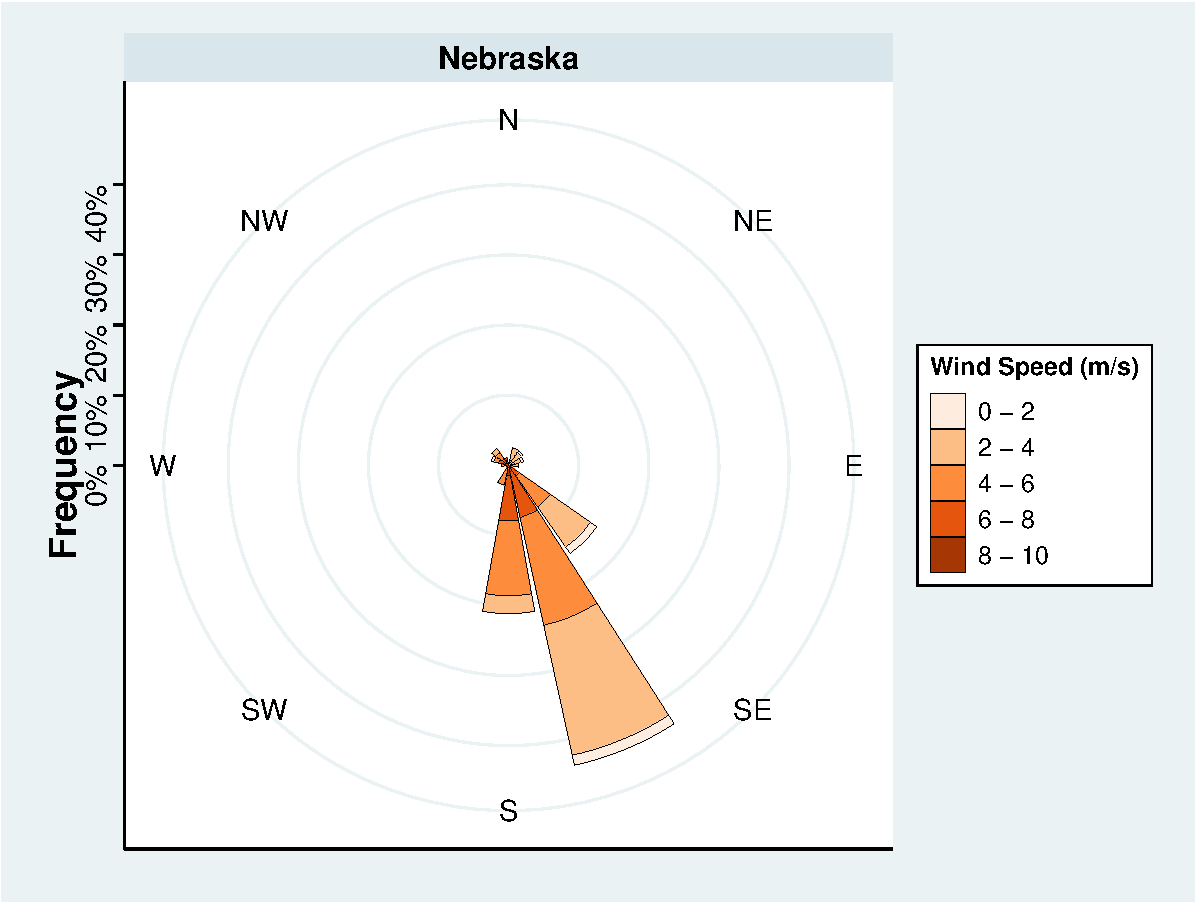
\includegraphics{Report_Dicamba_study_files/figure-latex/unnamed-chunk-64-1.pdf}
\caption{Wind rose plots demonstrating the average wind frequency (\%)
and wind speed (m s\textsuperscript{1}) grouped in 22.5° of direction
(from which the wind is blowing) in Nebraska.}
\end{figure}

\pagebreak
\newpage

\subsection{Transects}\label{transects-3}

\begin{figure}[h]

{\centering 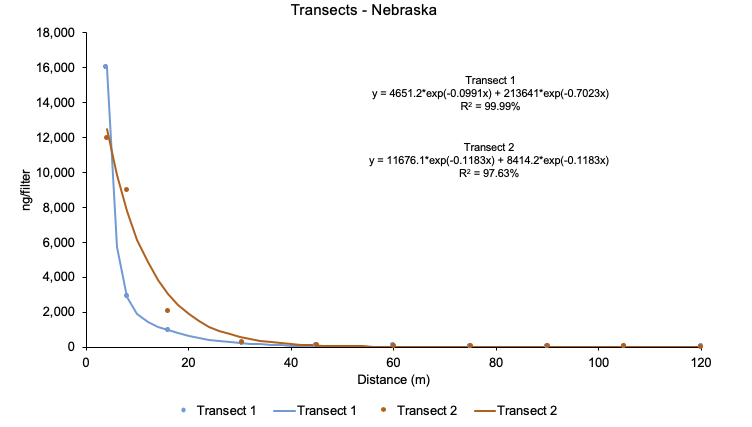
\includegraphics[width=1\linewidth]{Ntransect} 

}

\caption{Deposition of dicamba particles at the transects in Nebraska}\label{fig:unnamed-chunk-65}
\end{figure}

\pagebreak
\newpage

\subsection{Results at 21 DAT}\label{results-at-21-dat-2}

\subsubsection{Non-Xtend soybean injury
(\%)}\label{non-xtend-soybean-injury}

\paragraph{Area 1 (cover or uncover)}\label{area-1-cover-or-uncover}

\begin{longtable}[]{@{}lllll@{}}
\caption{Parameters of the log-logistic model at the area 1 (cover and
uncover) at 21 DAT in Nebraska.}\tabularnewline
\toprule
Parameter & Area & Estimate (± SE) & t-value & p-value\tabularnewline
\midrule
\endfirsthead
\toprule
Parameter & Area & Estimate (± SE) & t-value & p-value\tabularnewline
\midrule
\endhead
Slope & Cover & -85.48 ± 213.36 & -.40 & 0.69\tabularnewline
Slope & Uncover & 26.51 ± 275.86 & 0.09 & 0.92\tabularnewline
Lower limit & Cover & 35.83 ± 0.65 & 54.32 & 0.00 ***\tabularnewline
Lower limit & Uncover & 44.99 ± 0.68 & 65.27 & 0.00 ***\tabularnewline
Asymptote & Cover & 40.05 ± 1.39 & 28.65 & 0.00 ***\tabularnewline
Asymptote & Uncover & 65.03 ± 3.09 & 20.99 & 0.00 ***\tabularnewline
ED50 & Cover & 13.13 ± 1.81 & 7.22 & 0.00\tabularnewline
ED50 & Uncover & 5.85 ± 2.55 & 2.28 & 0.05 .\tabularnewline
\bottomrule
\end{longtable}

\begin{figure}
\centering
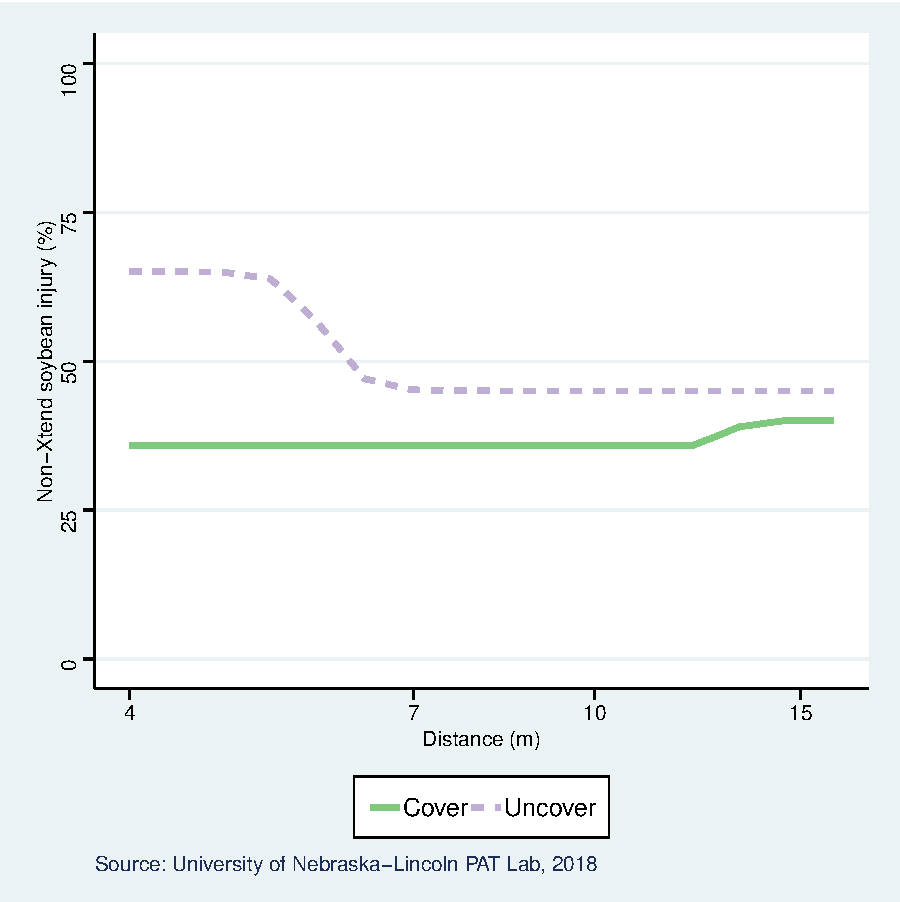
\includegraphics{Report_Dicamba_study_files/figure-latex/unnamed-chunk-68-1.pdf}
\caption{Non-Xtend soybean injury (\%) with distance (\%) from the
dicamba treated area in the downwind area 1 (cover and uncover) at 21
DAT in Nebraska.}
\end{figure}

\newpage

\paragraph{Area 2 (cover and uncover)}\label{area-2-cover-and-uncover}

\begin{longtable}[]{@{}lllll@{}}
\caption{Parameters of the log-logistic model at the Area 2 (cover and
uncover) at 21 DAT in Nebraska.}\tabularnewline
\toprule
Parameter & Area & Estimate (± SE) & t-value & p-value\tabularnewline
\midrule
\endfirsthead
\toprule
Parameter & Area & Estimate (± SE) & t-value & p-value\tabularnewline
\midrule
\endhead
Slope & Cover & 2.0 ± 9.21 & 0.21 & 0.82\tabularnewline
Slope & Uncover & 4.6 ± 5.42 & 0.84 & 0.40\tabularnewline
Lower limit & Cover & 5.4 ± 307.7 & 0.0 & 0.98\tabularnewline
Lower limit & Uncover & 40.2 ± 5.0 & 7.9 & 0.00 ***\tabularnewline
Asymptote & Cover & 39.2 ± 15.4 & 2.5 & 0.02 *\tabularnewline
Asymptote & Uncover & 67.3 ± 15.26 & 4.4 & 0.00 ***\tabularnewline
ED50 & Cover & 20.1 ± 156.5 & 0.1 & 0.90\tabularnewline
ED50 & Uncover & 6.6 ± 1.65 & 3.9 & 0.0 ***\tabularnewline
\bottomrule
\end{longtable}

\begin{figure}
\centering
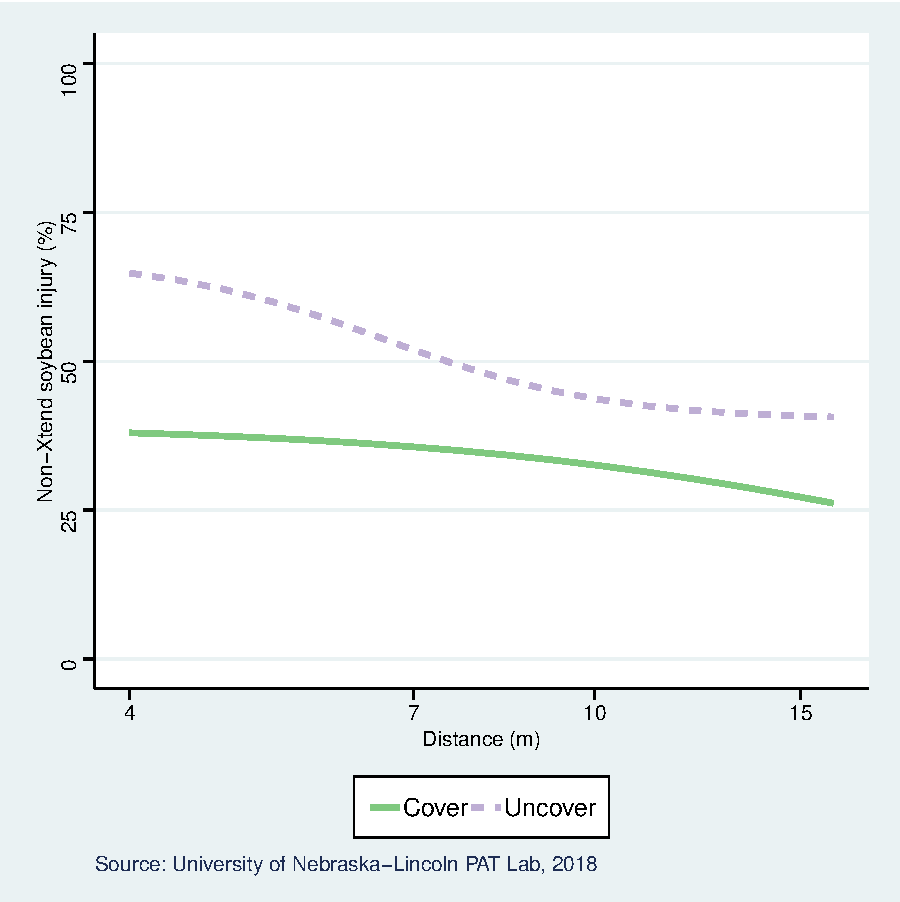
\includegraphics{Report_Dicamba_study_files/figure-latex/unnamed-chunk-71-1.pdf}
\caption{Non-Xtend soybean injury (\%) with distance (\%) from the
dicamba treated area in the downwind area 2 (cover and uncover) at 21
DAT in Nebraska.}
\end{figure}

\newpage

\subsubsection{Area 3 (cover and
uncover)}\label{area-3-cover-and-uncover}

\begin{longtable}[]{@{}lllll@{}}
\caption{Parameters of the log-logistic model at the Area 3 (cover and
uncover) at 21 DAT in Nebraska.}\tabularnewline
\toprule
Parameter & Area & Estimate (± SE) & t-value & p-value\tabularnewline
\midrule
\endfirsthead
\toprule
Parameter & Area & Estimate (± SE) & t-value & p-value\tabularnewline
\midrule
\endhead
Slope & Cover & 10.5 ± 16.7 & 0.6 & 0.53\tabularnewline
Slope & Uncover & 1.92 ± 7.26 & 0.26 & 0.79\tabularnewline
Lower limit & Cover & 25.3 ± 9.0 & 2.8 & 0.00 **\tabularnewline
Lower limit & Uncover & 38.5 ± 34.55 & 1.11 & 0.27\tabularnewline
Asymptote & Cover & 47.16 ± 4.54 & 10.4 & 0.00 ***\tabularnewline
Asymptote & Uncover & 120.3 ± 548.1 & 0.21 & 0.82\tabularnewline
ED50 & Cover & 10.7 ± 1.54 & 6.88 & 0.00 ***\tabularnewline
ED50 & Uncover & 4.84 ± 29.2 & 0.16 & 0.86\tabularnewline
\bottomrule
\end{longtable}

\begin{figure}
\centering
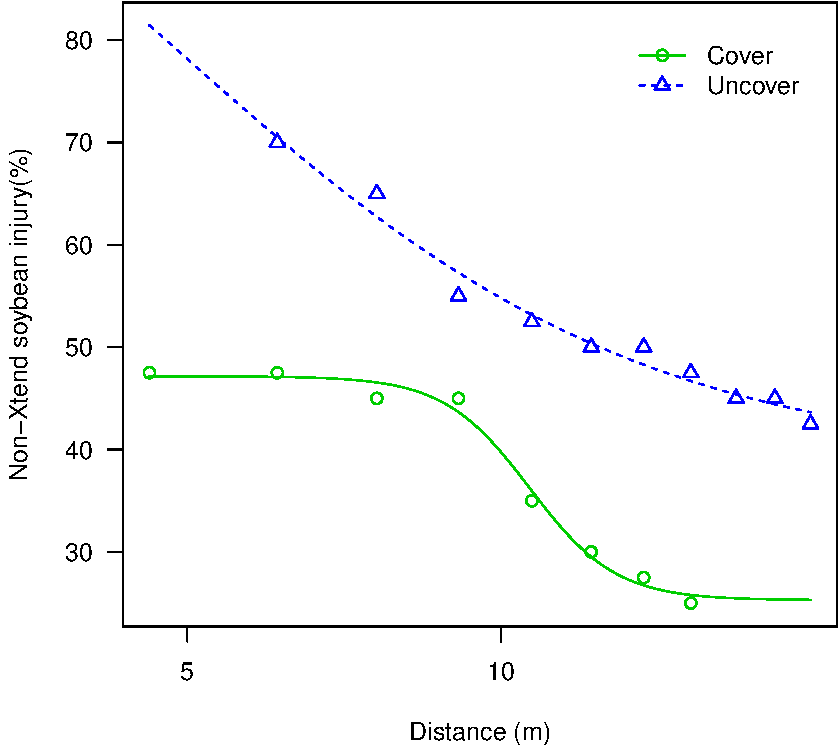
\includegraphics{Report_Dicamba_study_files/figure-latex/unnamed-chunk-74-1.pdf}
\caption{Non-Xtend soybean injury (\%) with distance (\%) from the
dicamba treated area in the downwind area 3 (cover and uncover) at 21
DAT in Nebraska.}
\end{figure}

\begin{figure}
\centering
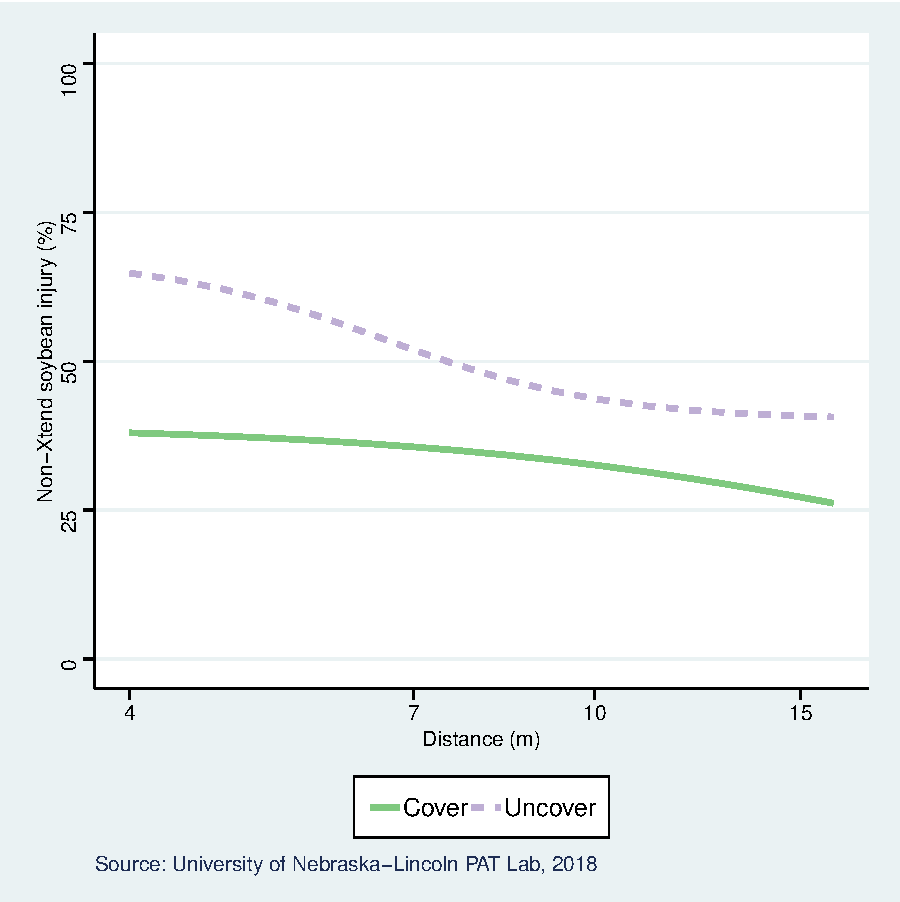
\includegraphics{Report_Dicamba_study_files/figure-latex/unnamed-chunk-75-1.pdf}
\caption{Non-Xtend soybean injury (\%) with distance (\%) from the
dicamba treated area in the downwind area 3 (cover and uncover) at 21
DAT in Nebraska.}
\end{figure}

\newpage

\pagebreak

\subsubsection{Non-Xtend soybeans
height}\label{non-xtend-soybeans-height-4}

There is no model convergence for Non-Xtend soybean height.

\paragraph{Area located at 1 (cover and
uncover)}\label{area-located-at-1-cover-and-uncover}

\begin{figure}
\centering
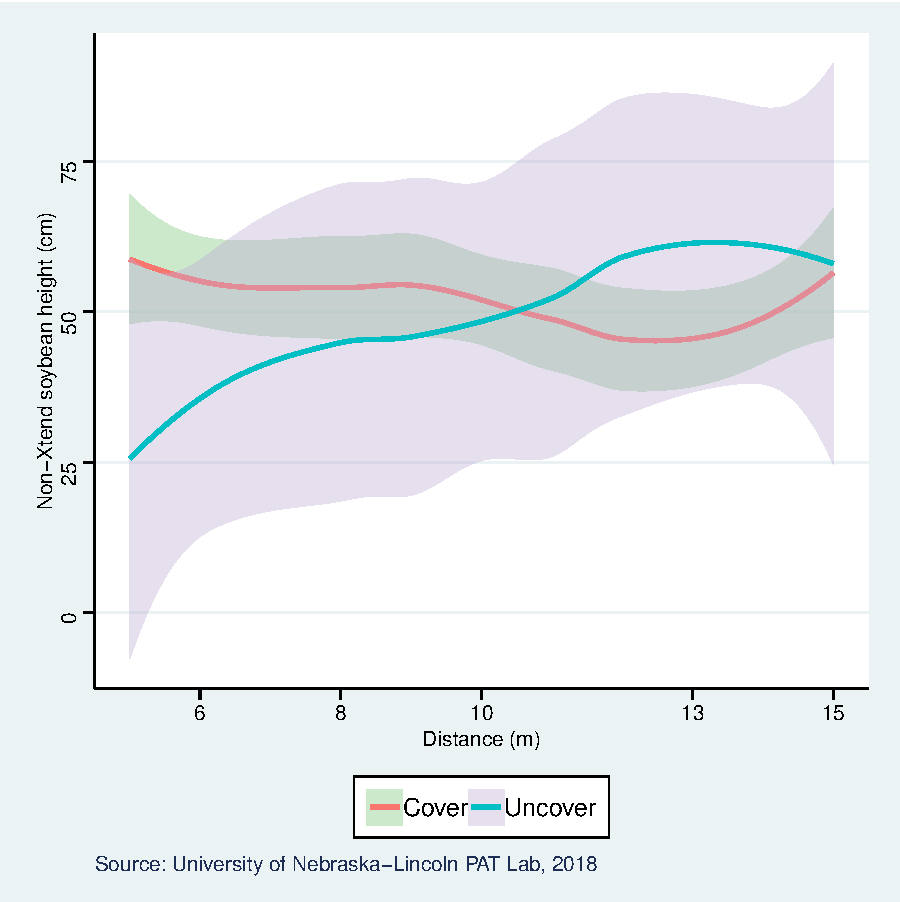
\includegraphics{Report_Dicamba_study_files/figure-latex/unnamed-chunk-76-1.pdf}
\caption{Non-Xtend soybean height (cm) with distance (\%) from the
dicamba treated area 1 (cover and uncover) at 21 DAT in Nebraska.}
\end{figure}

\newpage

\pagebreak

\paragraph{Area located at 2 (cover and
uncover)}\label{area-located-at-2-cover-and-uncover}

\begin{figure}
\centering
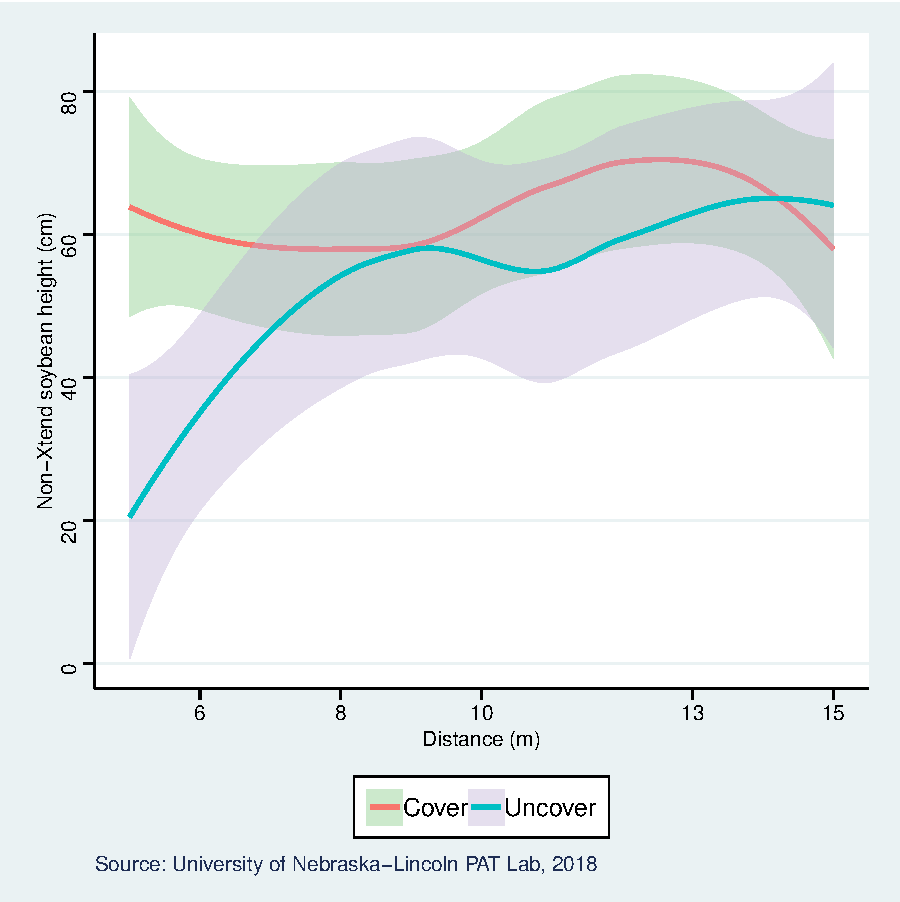
\includegraphics{Report_Dicamba_study_files/figure-latex/unnamed-chunk-77-1.pdf}
\caption{Non-Xtend soybean height (cm) with distance (\%) from the
dicamba treated area 2 (cover and uncover) at 21 DAT in Nebraska.}
\end{figure}

\newpage

\pagebreak

\paragraph{Area located at 3 (cover and
uncover)}\label{area-located-at-3-cover-and-uncover}

\begin{figure}
\centering
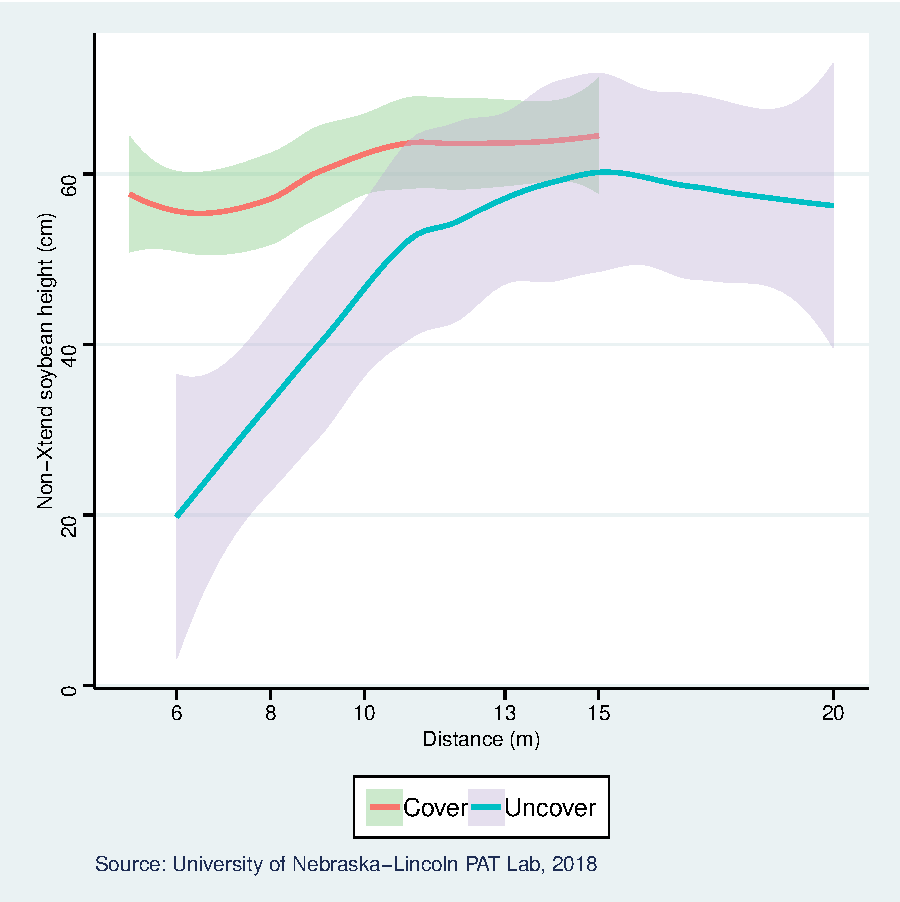
\includegraphics{Report_Dicamba_study_files/figure-latex/unnamed-chunk-78-1.pdf}
\caption{Non-Xtend soybean height (cm) with distance (\%) from the
dicamba treated area 3 (cover and uncover) at 21 DAT in Nebraska.}
\end{figure}

\newpage

\pagebreak

\section{ONTARIO}\label{ontario-1}

\subsection{Location}\label{location-4}

The study was conducted in a soybean field at Dresden, Ontario in Canada
(Figure X).

\begin{figure}[h]

{\centering 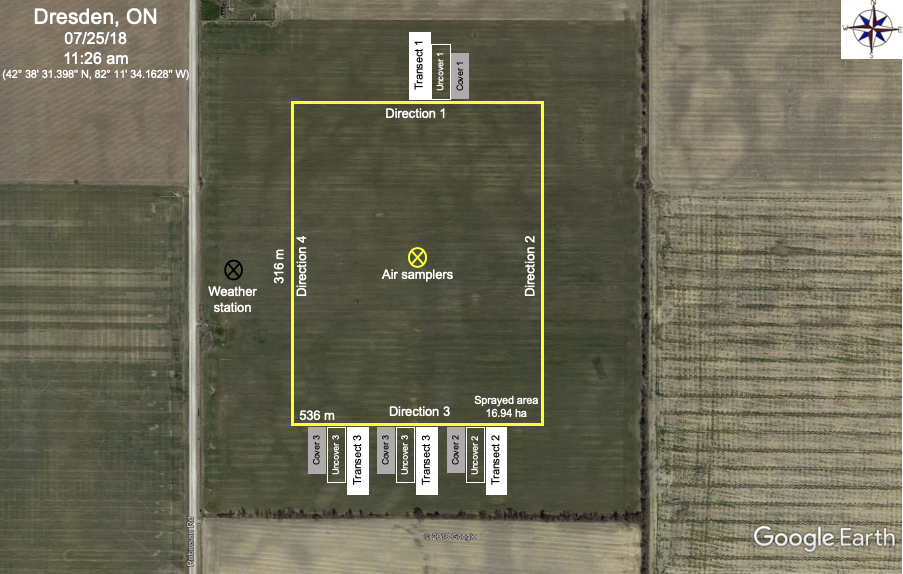
\includegraphics[width=1\linewidth]{Ontario} 

}

\caption{Aerial view of the large scale volatility trial in Ontario.}\label{fig:unnamed-chunk-80}
\end{figure}

\pagebreak

\subsection{Modeling}\label{modeling-4}

Non-Xtend \textbf{soybean injury (\%)} (visual data) from Ontario
presented here was collected in from one soybean plant
distance\textsuperscript{-1} at 21 DAT but without replication.
Nonetheless, we use the three-parameter logistic model (Equation 1) for
fitting soybean injury (\%) with distance from the area treated with
dicamba.

Equation 1: \[Y= \frac{d}{(1 + exp[b(logx - loge)]} \]

where \emph{Y} is the soybean injury (\%), \emph{x} is the distance (m)
from the dicamba treated area. in The parameter \emph{d} is the upper
limit (asymptote), \emph{b} is the slope and the parameter \emph{e} is
the ED50 (effective \emph{x} that causes 50\% reduction in \emph{Y}).
The upper limit of the model is locked at 100. Only data recorded 21 DAT
is presented.

Non-Xtend \textbf{soybean height} (cm) from Ontario presented here was
collected from 10 soybean plant distance\textsuperscript{-1} at 21 DAT.
\emph{Loess} local regression was fitted to the data.

\pagebreak
\newpage

\subsection{Wind}\label{wind-4}

Frequency of wind direction and speed (m/s) three days after dicamaba
application (Figure X).

\begin{figure}
\centering
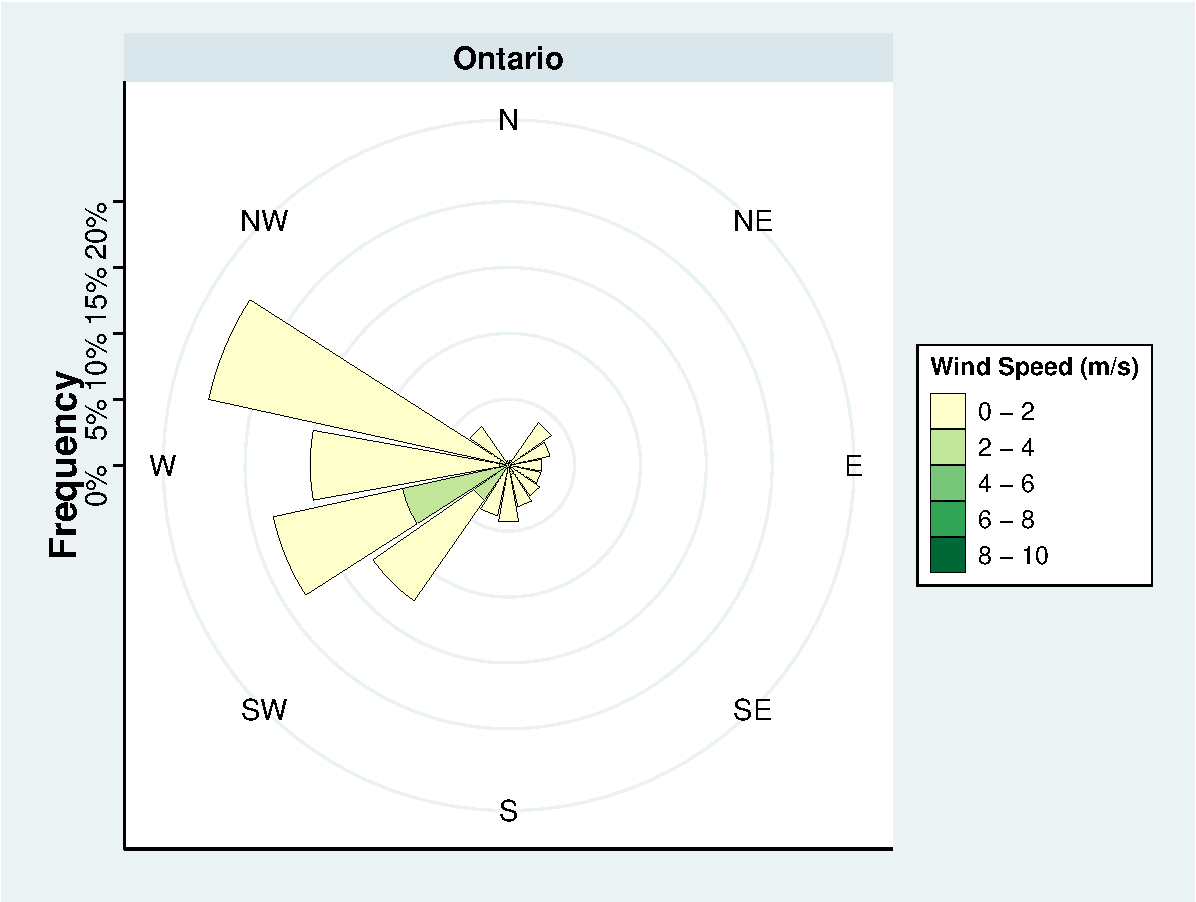
\includegraphics{Report_Dicamba_study_files/figure-latex/unnamed-chunk-82-1.pdf}
\caption{Wind rose plots demonstrating the average wind frequency (\%)
and wind speed (m s\textsuperscript{1}) grouped in 22.5° of direction
(from which the wind is blowing) in Ontario.}
\end{figure}

\pagebreak
\newpage

\subsection{Transects}\label{transects-4}

\begin{figure}[h]

{\centering 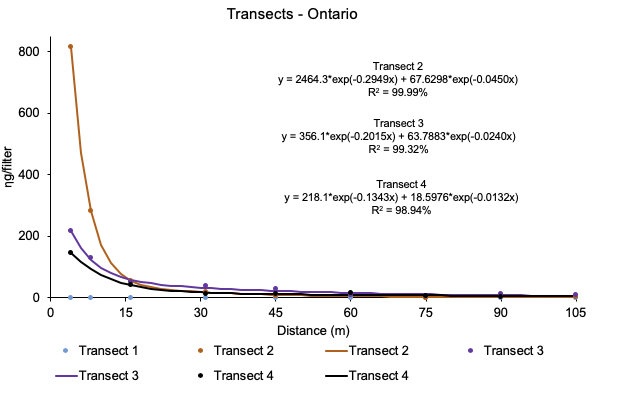
\includegraphics[width=1\linewidth]{ONtransect} 

}

\caption{Deposition of dicamba particles at the transects in Ontario}\label{fig:unnamed-chunk-83}
\end{figure}

\newpage

\pagebreak

\subsection{Results at 21 DAT}\label{results-at-21-dat-3}

\subsubsection{\texorpdfstring{Area located in the \textbf{Cover}
location.}{Area located in the Cover location.}}\label{area-located-in-the-cover-location.}

No injury was observed under the covered area of non-Xtend soybean.

\newpage

\pagebreak

\subsubsection{\texorpdfstring{Area located in the \textbf{Uncover}
location.}{Area located in the Uncover location.}}\label{area-located-in-the-uncover-location.}

\begin{longtable}[]{@{}lllll@{}}
\caption{Parameters of the log-logistic model of uncover area (1, 2, 3)
at 21 DAT in Ontario.}\tabularnewline
\toprule
Parameter & Uncover & Estimate (± SE) & t-value & p-value\tabularnewline
\midrule
\endfirsthead
\toprule
Parameter & Uncover & Estimate (± SE) & t-value & p-value\tabularnewline
\midrule
\endhead
Slope & 1 & 17.02 ± 38.02 & 0.55 & 0.65\tabularnewline
Slope & 2 & 3.81 ± 0.29 & 12.9 & 0.00 ***\tabularnewline
Slope & 3 & 18.8 ± 38.9 & 0.48 & 0.63\tabularnewline
Asymptote & 1 & 18.0 ± 0.26 & 68.2 & 0.00 ***\tabularnewline
Asymptote & 2 & 16.3 ± 0.53 & 30.6 & 0.00 ***\tabularnewline
Asymptote & 3 & 9.99 ± 0.26 & 37.9 & 0.00 ***\tabularnewline
ED50 & 1 & 9.73 ± 0.58 & 16.8 & 0.00 ***\tabularnewline
ED50 & 2 & 9.36 ± 0.29 & 31.8 & 0.00 ***\tabularnewline
ED50 & 3 & 10.5 ± 0.97 & 10.7 & 0.00 ***\tabularnewline
\bottomrule
\end{longtable}

\begin{longtable}[]{@{}llll@{}}
\caption{Estimation of the distance (m) that resulted in 1 (ED1), 10
(ED10), and 20\% (ED20) injury on non-Xtend soybeans of uncover area (1,
2, 3) at 21 DAT in Ontario.}\tabularnewline
\toprule
Uncover & ED1 (m) (± SE) & ED10 (m) (± SE) & ED20 (m) (±
SE)\tabularnewline
\midrule
\endfirsthead
\toprule
Uncover & ED1 (m) (± SE) & ED10 (m) (± SE) & ED20 (m) (±
SE)\tabularnewline
\midrule
\endhead
1 & 11.5 ± 3.59 & 9.61 ± 0.85 & NA ± NA\tabularnewline
2 & 19.1 ± 0.70 & 8.31 ± 0.32 & NA ± NA\tabularnewline
3 & 11.75 ± 3.94 & NA ± NA & NA ± NA\tabularnewline
\bottomrule
\end{longtable}

\begin{longtable}[]{@{}llll@{}}
\caption{Comparison of EDs among four sides of uncover area (1, 2, 3) at
21 DAT in Ontario.}\tabularnewline
\toprule
Comparison & Estimate (± SE) & t-value & p-value\tabularnewline
\midrule
\endfirsthead
\toprule
Comparison & Estimate (± SE) & t-value & p-value\tabularnewline
\midrule
\endhead
1/2:ED1/ED1 & 0.60 ± 0.18 & -2.11 & 0.05\tabularnewline
1/3:ED1/ED1 & 1.00 ± 0.21 & 6.55 & 0.00\tabularnewline
2/3:ED1/ED1 & 0.14 ± 0.13 & -6.47 & 0.00\tabularnewline
1/2:ED10/ED10 & 1.15 ± 0.11 & 1.39 & 0.18\tabularnewline
1/3:ED10/ED10 & NA & NA & NA\tabularnewline
2/3:ED10/ED10 & NA & NA & NA\tabularnewline
1/2:ED20/ED20 & NA & NA & NA\tabularnewline
1/3:ED20/ED20 & NA & NA & NA\tabularnewline
2/3:ED20/ED20 & NA & NA & NA\tabularnewline
\bottomrule
\end{longtable}

\begin{figure}
\centering
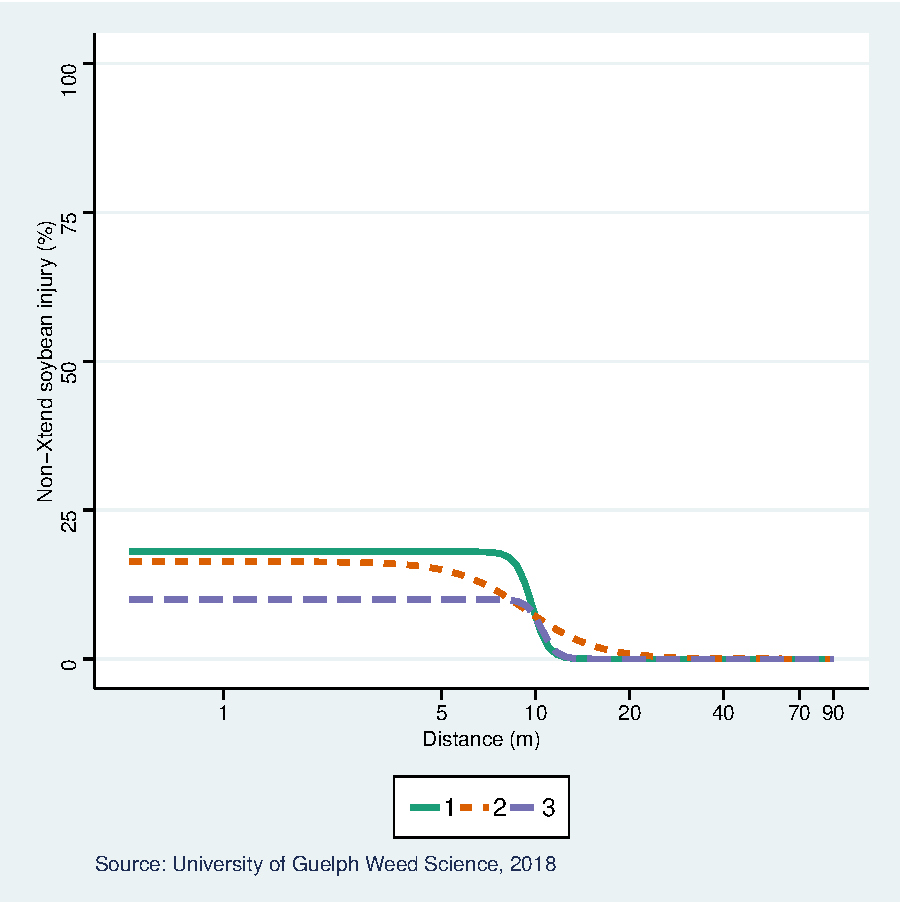
\includegraphics{Report_Dicamba_study_files/figure-latex/ONPlot-1.pdf}
\caption{Non-Xtend soybean injury (\%) with distance (\%) from the
dicamba treated area oof uncover area (1, 2, 3) at 21 DAT in Ontario.}
\end{figure}

\newpage

\pagebreak

\subsubsection{Non-Xtend soybeans
height}\label{non-xtend-soybeans-height-5}

There is no model convergence for Non-Xtend soybean height.

\paragraph{Area located at 1 (cover and
uncover)}\label{area-located-at-1-cover-and-uncover-1}

\begin{figure}
\centering
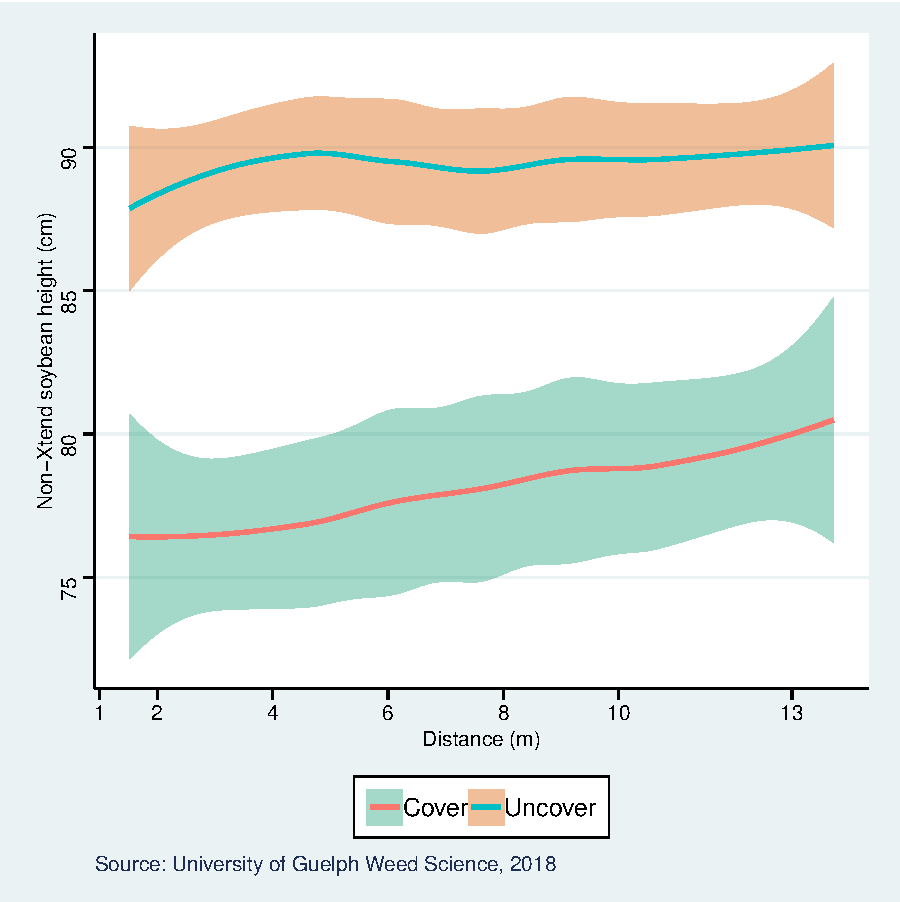
\includegraphics{Report_Dicamba_study_files/figure-latex/unnamed-chunk-85-1.pdf}
\caption{Non-Xtend soybean height (cm) with distance (\%) from the
dicamba treated area 1 (cover and uncover) at 21 DAT in Ontario.}
\end{figure}

\newpage

\pagebreak

\paragraph{Area located at 2 (cover and
uncover)}\label{area-located-at-2-cover-and-uncover-1}

\begin{figure}
\centering
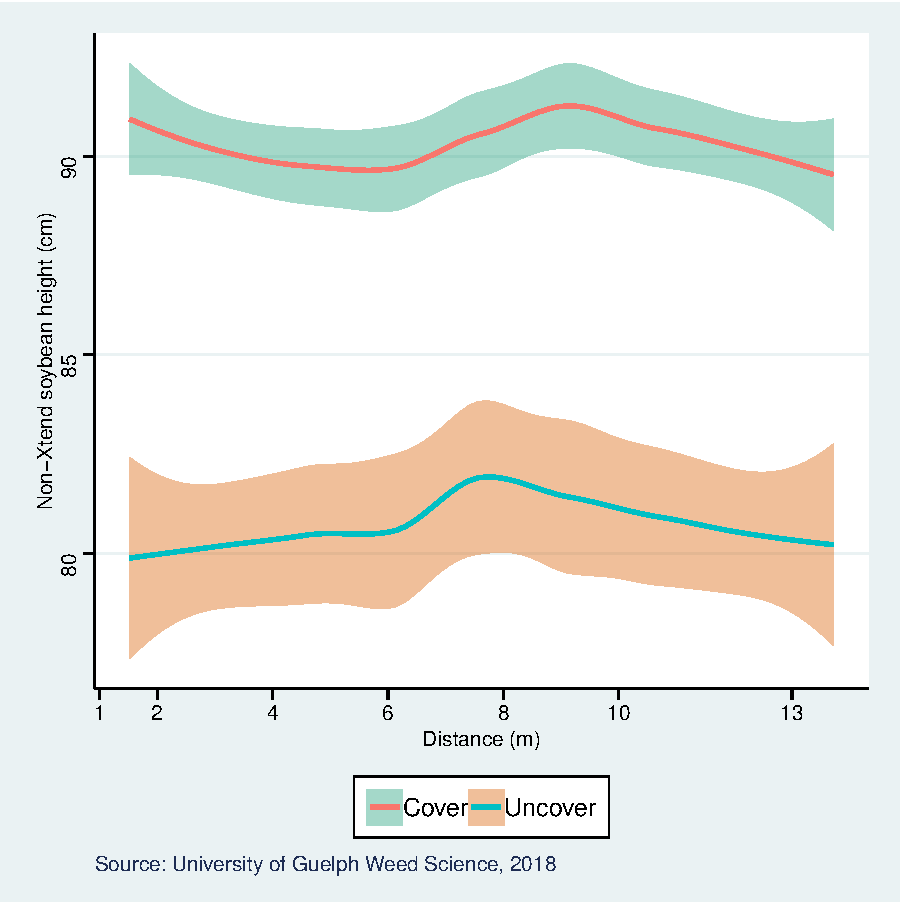
\includegraphics{Report_Dicamba_study_files/figure-latex/unnamed-chunk-86-1.pdf}
\caption{Non-Xtend soybean height (cm) with distance (\%) from the
dicamba treated area 2 (cover and uncover) at 21 DAT in Ontario.}
\end{figure}

\newpage

\pagebreak

\paragraph{Area located at 3 (cover and
uncover)}\label{area-located-at-3-cover-and-uncover-1}

\begin{figure}
\centering
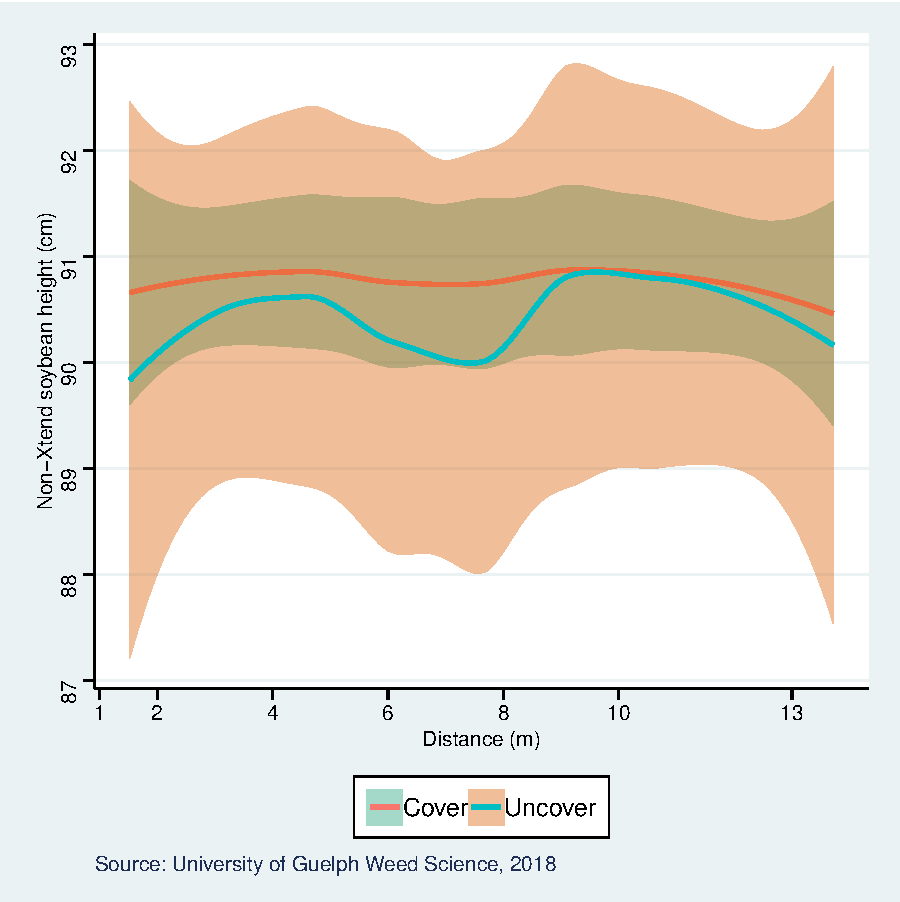
\includegraphics{Report_Dicamba_study_files/figure-latex/unnamed-chunk-87-1.pdf}
\caption{Non-Xtend soybean height (cm) with distance (\%) from the
dicamba treated area 2 (cover and uncover) at 21 DAT in Ontario.}
\end{figure}

\newpage

\pagebreak

\section{WISCONSIN}\label{wisconsin-1}

\subsection{Location}\label{location-5}

The study was conducted in a 8 acres soybean field at the University of
Wisconsin-Madison (Figure 1).

\begin{figure}[h]

{\centering \includegraphics[width=1\linewidth]{Wisconsin} 

}

\caption{Aerial view of the large scale volatility trial in Wisconsin.}\label{fig:unnamed-chunk-89}
\end{figure}

\pagebreak

\subsection{Modeling}\label{modeling-5}

Non-Xtend \textbf{soybean injury (\%)} (visual data) from Wisconsin
presented here was collected from three diferent (replications) soybean
plant distance\textsuperscript{-1} at 28 DAT. Therefore, we use the
three-parameter logistic model (Equation 1) for fitting soybean injury
(\%) with distance from the area treated with dicamba.

Equation 1: \[Y= \frac{d}{(1 + exp[b(logx - loge)]} \]

where \emph{Y} is the soybean injury (\%), \emph{x} is the distance (m)
from the dicamba treated area. in The parameter \emph{d} is the upper
limit (asymptote), \emph{b} is the slope and the parameter \emph{e} is
the ED50 (effective \emph{x} that causes 50\% reduction in \emph{Y}).
The upper limit of the model is locked at 100. Only data recorded 21 DAT
is presented.

Non-Xtend \textbf{soybean height} (cm) from Wisconsin presented here was
collected from 10 soybean plant distance\textsuperscript{-1} at 28 DAT.
\emph{Loess} local regression was fitted to the data.

\pagebreak
\newpage

\subsection{Wind}\label{wind-5}

Frequency of wind direction and speed (m/s) three days after dicamaba
application (Figure X).

\begin{figure}
\centering
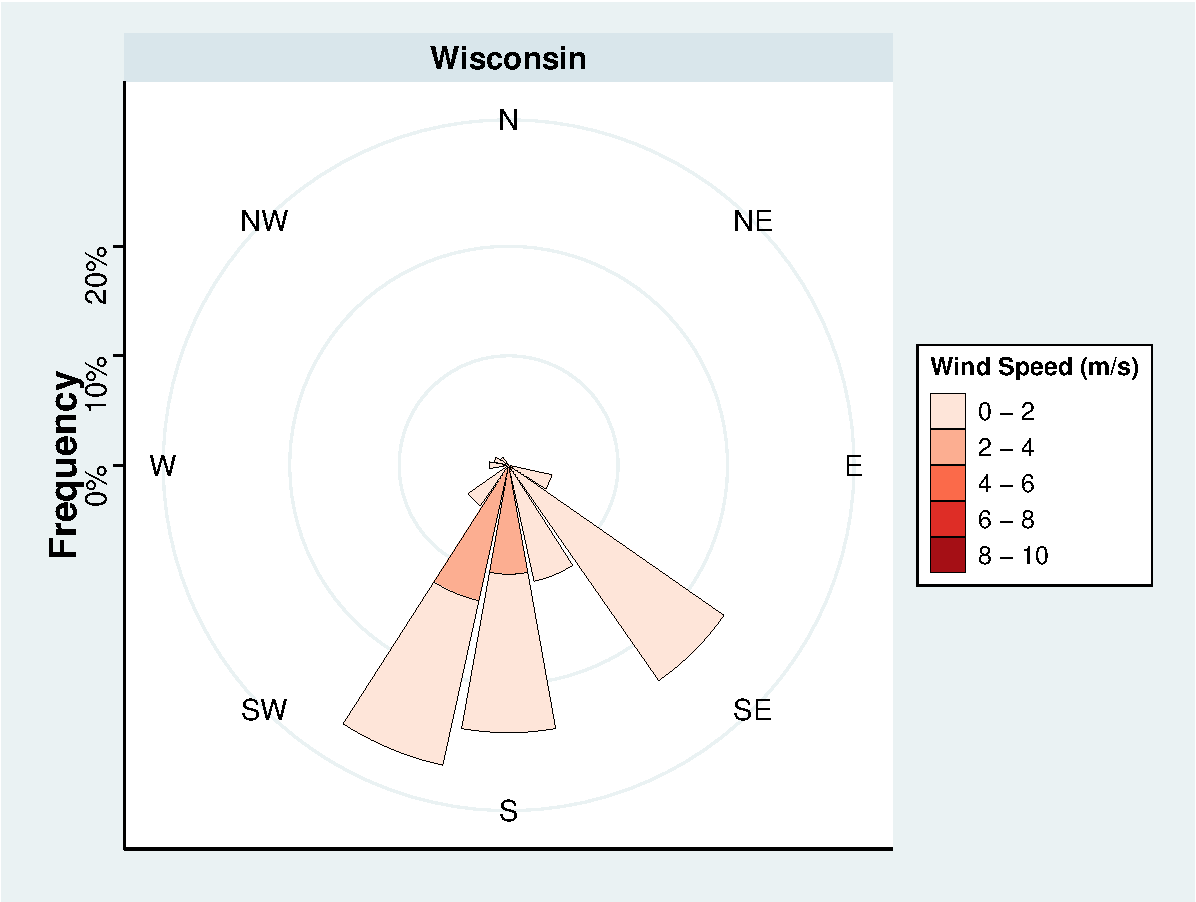
\includegraphics{Report_Dicamba_study_files/figure-latex/unnamed-chunk-91-1.pdf}
\caption{Wind rose plots demonstrating the average wind frequency (\%)
and wind speed (m s\textsuperscript{1}) grouped in 22.5° of direction
(from which the wind is blowing) in Wisconsin.}
\end{figure}

\pagebreak
\newpage

\subsection{Transects}\label{transects-5}

\begin{figure}[h]

{\centering 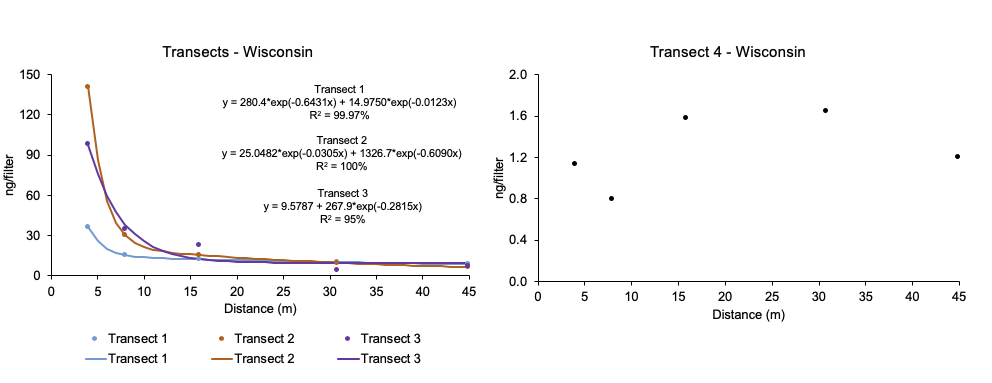
\includegraphics[width=1\linewidth]{Wisctransect} 

}

\caption{Deposition of dicamba particles at the transects in Wisconsin}\label{fig:unnamed-chunk-92}
\end{figure}

\pagebreak
\newpage

\subsection{Results at 28 DAT}\label{results-at-28-dat}

\subsubsection{Non-Xtend soybean
injury}\label{non-xtend-soybean-injury-1}

\paragraph{Area located in the northwest of the dicamba treated block
(N-1)}\label{area-located-in-the-northwest-of-the-dicamba-treated-block-n-1}

\begin{longtable}[]{@{}lllll@{}}
\caption{Parameters of the log-logistic model at the N-1 (cover and
uncover) at 28 DAT in Wisconsin.}\tabularnewline
\toprule
Parameter & Area & Estimate (± SE) & t-value & p-value\tabularnewline
\midrule
\endfirsthead
\toprule
Parameter & Area & Estimate (± SE) & t-value & p-value\tabularnewline
\midrule
\endhead
Slope & Cover & 2.03 ± 0.15 & 13.5 & 0.00 ***\tabularnewline
Slope & Uncover & 2.99 ± 0.19 & 13.45 & 0.00 ***\tabularnewline
Asymptote & Cover & 42.38 ± 1.19 & 35.5 & 0.00 ***\tabularnewline
Asymptote & Uncover & 43.63 ± 0.92 & 47.2 & 0.00 ***\tabularnewline
ED50 & Cover & 3.94 ± 0.18 & 21.0 & 0.00 ***\tabularnewline
ED50 & Uncover & 5.80 ± 0.15 & 38.3 & 0.00 ***\tabularnewline
\bottomrule
\end{longtable}

\begin{longtable}[]{@{}llll@{}}
\caption{Estimation of the distance (m) that resulted in 1 (ED1), 10
(ED10), and 20\% (ED20) injury on non-Xtend soybeans at the N-1 (cover
and uncover) at 28 DAT in Wisconsin.}\tabularnewline
\toprule
Area & ED1 (m) (± SE) & ED10 (m) (± SE) & ED20 (m)(± SE)\tabularnewline
\midrule
\endfirsthead
\toprule
Area & ED1 (m) (± SE) & ED10 (m) (± SE) & ED20 (m)(± SE)\tabularnewline
\midrule
\endhead
Uncover & 20.3 ± 1.40 & 8.70 ± 0.21 & 6.13 ± 0.14\tabularnewline
Cover & 24.69 ± 2.63 & 7.04 ± 0.24 & 4.17 ± 0.18\tabularnewline
\bottomrule
\end{longtable}

\begin{longtable}[]{@{}llll@{}}
\caption{Comparison of EDs of non-Xtend soybeans at the N-1 (cover and
uncover) at 28 DAT in Wisconsin.}\tabularnewline
\toprule
Comparison & Estimate (± SE) & t-value & p-value\tabularnewline
\midrule
\endfirsthead
\toprule
Comparison & Estimate (± SE) & t-value & p-value\tabularnewline
\midrule
\endhead
Cover/Uncover:ED1/ED1 & 0.08 ± 0.11 & -1.48 & 0.13\tabularnewline
Cover/Uncover:ED10/ED10 & 1.23 ± 0.05 & 4.18 & 0.00\tabularnewline
Cover/Uncover:ED20/ED20 & 1.47 ± 0.08 & 5.86 & 0.00\tabularnewline
\bottomrule
\end{longtable}

\begin{figure}
\centering
\includegraphics{Report_Dicamba_study_files/figure-latex/unnamed-chunk-95-1.pdf}
\caption{Non-Xtend soybean injury (\%) with distance (\%) from the
dicamba treated area at N-1 (cover and uncover) in Wisconsin at 28 DAT.}
\end{figure}

\pagebreak

\subsubsection{Area located in the north (center) of the dicamba treated
block
(N-2)}\label{area-located-in-the-north-center-of-the-dicamba-treated-block-n-2}

\begin{longtable}[]{@{}lllll@{}}
\caption{Parameters of the log-logistic model at the N-2 (cover and
uncover) at 28 DAT in Wisconsin.}\tabularnewline
\toprule
Parameter & Area & Estimate (± SE) & t-value & p-value\tabularnewline
\midrule
\endfirsthead
\toprule
Parameter & Area & Estimate (± SE) & t-value & p-value\tabularnewline
\midrule
\endhead
Slope & Cover & 3.73 ± 0.31 & 11.7 & 0.00 ***\tabularnewline
Slope & Uncover & 3.47 ± 0.23 & 15.3 & 0.00 ***\tabularnewline
Asymptote & Cover & 40.2 ± 1.0 & 39.8 & 0.00 ***\tabularnewline
Asymptote & Uncover & 44.9 ± 0.92 & 48.3 & 0.00 ***\tabularnewline
ED50 & Cover & 3.3 ± 0.1 & 31.6 & 0.00 ***\tabularnewline
ED50 & Uncover & 5.66 ± 0.13 & 40.9 & 0.00 ***\tabularnewline
\bottomrule
\end{longtable}

\begin{longtable}[]{@{}llll@{}}
\caption{Estimation of the distance (m) that resulted in 1 (ED1), 10
(ED10), and 20\% (ED20) injury on non-Xtend soybeans at the N-2 (cover
and uncover) at 28 DAT in Wisconsin.}\tabularnewline
\toprule
Area & ED1 (m) (± SE) & ED10 (m) (± SE) & ED20 (m) (± SE)\tabularnewline
\midrule
\endfirsthead
\toprule
Area & ED1 (m) (± SE) & ED10 (m) (± SE) & ED20 (m) (± SE)\tabularnewline
\midrule
\endhead
Uncover & 16.79 ± 0.99 & 8.11 ± 0.2 & 6.03 ± 0.13\tabularnewline
Cover & 8.67 ± 0.59 & 4.37 ± 0.11 & 3.26 ± 0.10\tabularnewline
\bottomrule
\end{longtable}

\begin{longtable}[]{@{}llll@{}}
\caption{Comparison of EDs of non-Xtend soybeans at the N-1 (cover and
uncover) at 28 DAT in Wisconsin.}\tabularnewline
\toprule
Tarp & Estimate (± SE) & t-value & p-value\tabularnewline
\midrule
\endfirsthead
\toprule
Tarp & Estimate (± SE) & t-value & p-value\tabularnewline
\midrule
\endhead
Cover/Uncover:ED1/ED1 & 0.52 ± 0.04 & -10.3 & 0.00\tabularnewline
Cover/Uncover:ED10/ED10 & 0.53 ± 0.02 & -26.0 & 0.00\tabularnewline
Cover/Uncover:ED20/ED20 & 0.54 ± 0.02 & -22.0 & 0.00\tabularnewline
\bottomrule
\end{longtable}

\begin{figure}
\centering
\includegraphics{Report_Dicamba_study_files/figure-latex/unnamed-chunk-98-1.pdf}
\caption{Non-Xtend soybean injury (\%) with distance (\%) from the
dicamba treated area at N-2 (cover and uncover) in Wisconsin at 28 DAT.}
\end{figure}

\pagebreak

\subsubsection{Area located in the northeast of the dicamba treated
block
(N-3)}\label{area-located-in-the-northeast-of-the-dicamba-treated-block-n-3}

\begin{longtable}[]{@{}lllll@{}}
\caption{Parameters of the log-logistic model at the N-3 (cover and
uncover) at 28 DAT in Wisconsin.}\tabularnewline
\toprule
Parameter & Tarp & Estimate (± SE) & t-value & p-value\tabularnewline
\midrule
\endfirsthead
\toprule
Parameter & Tarp & Estimate (± SE) & t-value & p-value\tabularnewline
\midrule
\endhead
Slope & Cover & 2.34 ± 0.13 & 17.7 & 0.00 ***\tabularnewline
Slope & Uncover & 2.6 ± 0.12 & 20.9 & 0.00 ***\tabularnewline
Asymptote & Cover & 38.9 ± 0.9 & 41.7 & 0.00 ***\tabularnewline
Asymptote & Uncover & 43.73 ± 0.9 & 50.4 & 0.00 ***\tabularnewline
ED50 & Cover & 2.34 ± 0.08 & 26.1 & 0.00 ***\tabularnewline
ED50 & Uncover & 4.19 ± 0.11 & 37.9 & 0.00 ***\tabularnewline
\bottomrule
\end{longtable}

\begin{longtable}[]{@{}llll@{}}
\caption{Estimation of the distance (m) that resulted in 1 (ED1), 10
(ED10), and 20\% (ED20) injury on non-Xtend soybeans at the N-3 (cover
and uncover) at 28 DAT in Wisconsin.}\tabularnewline
\toprule
Tarp & ED1 (m) (± SE) & ED10 (m) (± SE) & ED20 (m) (± SE)\tabularnewline
\midrule
\endfirsthead
\toprule
Tarp & ED1 (m) (± SE) & ED10 (m) (± SE) & ED20 (m) (± SE)\tabularnewline
\midrule
\endhead
Uncover & 17.7 ± 0.9 & 6.7 ± 0.13 & 4.5 ± 0.14\tabularnewline
Cover & 11.1 ± 0.8 & 3.7 ± 0.11 & 2.3 ± 0.1\tabularnewline
\bottomrule
\end{longtable}

\begin{longtable}[]{@{}llll@{}}
\caption{Comparison of EDs of non-Xtend soybeans at the N-1 (cover and
uncover) at 28 DAT in Wisconsin.}\tabularnewline
\toprule
Comparison & Estimate (± SE) & t-value & p-value\tabularnewline
\midrule
\endfirsthead
\toprule
Comparison & Estimate (± SE) & t-value & p-value\tabularnewline
\midrule
\endhead
Cover/Uncover:ED1/ED1 & 0.62 ± 0.05 & -6.7 & 0.00\tabularnewline
Cover/Uncover:ED10/ED10 & 0.55 ± 0.01 & -22.4 & 0.00\tabularnewline
Cover/Uncover:ED20/ED20 & -0.51 ± 0.02 & -20.7 & 0.00\tabularnewline
\bottomrule
\end{longtable}

\begin{figure}
\centering
\includegraphics{Report_Dicamba_study_files/figure-latex/unnamed-chunk-101-1.pdf}
\caption{Non-Xtend soybean injury (\%) with distance (\%) from the
dicamba treated area at N-3 (cover and uncover) in Wisconsin at 28 DAT.}
\end{figure}

\pagebreak

\paragraph{Area located in the south (upwind) of the dicamba treated
block
(S-1)}\label{area-located-in-the-south-upwind-of-the-dicamba-treated-block-s-1}

This tarp area showed low or no injury on non-Xtend soybean (upwind
direction). Therefore, the present the raw data.

\begin{figure}
\centering
\includegraphics{Report_Dicamba_study_files/figure-latex/unnamed-chunk-103-1.pdf}
\caption{Non-Xtend soybean injury (\%) with distance (m) from the
dicamba treated area at S-1 (cover and uncover) in Wisconsin at 28 DAT.}
\end{figure}

\pagebreak
\newpage

\subsubsection{Non-Xtend soybean height}\label{non-xtend-soybean-height}

\paragraph{Area located in the northwest of the dicamba treated block
(N-1)}\label{area-located-in-the-northwest-of-the-dicamba-treated-block-n-1-1}

\begin{verbatim}
## Warning: Removed 3 rows containing non-finite values (stat_smooth).
\end{verbatim}

\begin{figure}
\centering
\includegraphics{Report_Dicamba_study_files/figure-latex/unnamed-chunk-104-1.pdf}
\caption{Non-Xtend soybean height (cm) with distance (\%) from the
dicamba treated area at N-1 (cover and uncover) in Wisconsin at 28 DAT.}
\end{figure}

\pagebreak
\newpage

\paragraph{Area located in the north (center) of the dicamba treated
block
(N-2)}\label{area-located-in-the-north-center-of-the-dicamba-treated-block-n-2-1}

\begin{figure}
\centering
\includegraphics{Report_Dicamba_study_files/figure-latex/unnamed-chunk-105-1.pdf}
\caption{Non-Xtend soybean height (cm) with distance (\%) from the
dicamba treated area at N-2 (cover and uncover) in Wisconsin at 28 DAT.}
\end{figure}

\pagebreak
\newpage

\subsubsection{Area located in the northeast of the dicamba treated
block
(N-3)}\label{area-located-in-the-northeast-of-the-dicamba-treated-block-n-3-1}

\begin{figure}
\centering
\includegraphics{Report_Dicamba_study_files/figure-latex/unnamed-chunk-106-1.pdf}
\caption{Non-Xtend soybean height (cm) with distance (\%) from the
dicamba treated area at N-3 (cover and uncover) in Wisconsin at 28 DAT.}
\end{figure}

\pagebreak
\newpage

\paragraph{Area located in the south (upwind) of the dicamba treated
block
(S-1)}\label{area-located-in-the-south-upwind-of-the-dicamba-treated-block-s-1-1}

\begin{figure}
\centering
\includegraphics{Report_Dicamba_study_files/figure-latex/unnamed-chunk-107-1.pdf}
\caption{Non-Xtend soybean height (cm) with distance (\%) from the
dicamba treated area at S-1 (cover and uncover) in Wisconsin at 28 DAT.}
\end{figure}


\end{document}
